\documentclass[lletterpaper,12pt]{report}
\usepackage[letterpaper,paperheight=26cm, paperwidth=20cm, top=1.5cm,bottom=1.5cm, left=2cm, right=2cm]{geometry}
%\geometry{}
\columnseprule1pt
\columnsep0.7cm
\usepackage{makeidx}
\usepackage[latin1]{inputenc}
%usepackage{german}
\usepackage{alltt}
\usepackage{verbatim}
\usepackage[dvipdfm]{color}
\usepackage[
    bookmarks,
    colorlinks,
    linkcolor=blue
]{hyperref}
\usepackage{epsfig}
\usepackage{graphicx}

\definecolor{grau}{rgb}{0.95, 0.95, 0.95}
\definecolor{gelb}{rgb}{0.95, 0.95, 0.5}
\definecolor{rot}{rgb}{0.95, 0.8, 0.8}
\definecolor{gruen}{rgb}{0.8, 0.95, 0.8}
\definecolor{blau}{rgb}{0.8, 0.8, 0.95}
\definecolor{rgxblau}{rgb}{0.0, 0.0, 0.5}
\definecolor{trmred}{rgb}{0.2, 0.1, 0.1}

\newenvironment{code}[0]{\verbatim}{\endverbatim}
\newcommand{\exq}[1]{\begin{quote}\begin{alltt}#1\end{alltt}\end
{quote}}
\newcommand{\ex}[1]{\begin{alltt}#1\end{alltt}}
\newcommand{\boxquote}[3]{
\begin{center}
\colorbox{#1}%
{\parbox{0.9\textwidth}{
\sf
\underline{#2}:
#3
}}
\end{center}}
\newcommand{\hasdiff}[1]{\boxquote{rot}{Difference to \haskell{} 98/2010}{#1}}
\newcommand{\note}[1]{\boxquote{grau}{Note}{#1}}
\newcommand{\todo}[1]{\boxquote{blau}{TODO}{#1}}
\newcommand{\trans}[1]{\boxquote{gelb}{Translation}{#1}}
\newcommand{\inmargin}[1]{\marginpar{\scriptsize\raggedright #1}}
\newcommand{\example}[1]{\boxquote{gruen}{Example}{#1}}

\newcommand{\haskell}[0]{\textsc{Haskell}}
\newcommand{\frege}[0]{\textsc{Frege}}
\newcommand{\java}[0]{\textsc{Java}}
\newcommand{\arrow}[0]{\begin{math}\rightarrow\end{math}}
\newcommand{\qq}[1]{"#1"}

\newcommand{\jex}[1]{\emph{\textcolor{rgxblau}{jex}}{\Large (}#1{\Large )}}
\newcommand{\ftn}[1]{\emph{\textcolor{rgxblau}{Ftn}}{\Large (}#1{\Large )}}
\newcommand{\jtn}[1]{\emph{\textcolor{rgxblau}{Jtn}}{\Large (}#1{\Large )}}
\newcommand{\unbox}[1]{#1\texttt{.unbox()}}
\newcommand{\tobox}[2]{\ftn{#1}\-\texttt{.box(}#2\texttt{)}}
\newcommand{\cons}[3] {\ftn{#1}\-\texttt{.new(#2 #3)}}

\newcommand{\term}[1]{\textbf{\texttt{\textcolor{trmred}{#1}}}}
\newcommand{\regex}[1]{\texttt{\textcolor{rgxblau}{#1}}}
\newcommand{\sym}[1]{\textbf{\texttt{\textcolor{trmred}{#1}}}}
\newcommand{\gcom}[1]{{\hspace{\fill}\scriptsize (#1)}}

\newcommand{\brackz}[0]{\textbf{\texttt{\textcolor{trmred}{]}}}}
\newcommand{\bracka}[0]{\textbf{\texttt{\textcolor{trmred}{[}}}}
\newcommand{\bracea}[0]{\textbf{\texttt{\textcolor{trmred}{\{}}}}
\newcommand{\bracez}[0]{\textbf{\texttt{\textcolor{trmred}{\}}}}}

\newcommand{\nont}[1]{\textit{#1}}
\newcommand{\some}[1]{{\Large \{}#1{\Large \}}}
\newcommand{\opt}[1]{{\Large [} #1 {\Large ]}}
\newcommand{\more}[1]{#1 {\Large \{} #1 {\Large \}}}
\newcommand{\liste}[2]{#1\some{#2 #1}}
\newcommand{\rul}[1]{\nont{#1}:\\\hspace{0.5in} }
\newcommand{\alt}[0]{\\\hspace{0.5in}{\Large $|$} }
\newcommand{\oder}[0]{{\Large $|$}}
\newcommand{\checked}[1]{#1!}

\makeindex

\parindent0cm
%\oddsidemargin0.5cm
%\evensidemargin0.5cm
%\textwidth12cm
\parskip2mm
\pagestyle{headings}

\date{last changed \today{} \\ 3.20.6}
\author{\small{by Ingo Wechsung}}
\title{The \frege{} Programming Language (\emph{Draft})}

% explained that Ord T needs a hashCode implementation.
% explicated inlining
% explicated why 2 sibling subclass instantiations may not work
% claified ambiguous instance imports.
% final (?) version of import
% corrected chaptermodules - classes can have no member lists
% listed protected an forall keywords in lex chapter
% corrected chaptermodules
% adapted chaptermodules and described new import features

\begin{document}

\maketitle


%\begingroup 
%\let\onecolumn\twocolumn 

\begin{abstract}

This document describes the functional programming language \frege{}
and its implementation
for the \java{} virtual machine. Commonplace features of \frege{} are
type inference,
lazy evaluation,
modularization and separate compile-ability,
algebraic data types and type classes,
pattern matching and list comprehension.

Distinctive features are, first, that the type system supports
\emph{higher ranked polymorphic types},
and, second,
that \frege{} code is compiled to \java{}.
This allows for maximal interoperability with existing
\java{} software.
Any \java{} class may be used as an abstract data type, \java{}
functions and methods may be called from \frege{} functions and vice
versa.

Despite this interoperability feature  \frege{} is a pure functional language as long as impure \java{} functions are declared accordingly.

\begin{center}\textbf{What is or who was Frege?}\end{center}

%\inmargin{In honor of \\G. Frege}
Friedrich Ludwig Gottlob Frege
\index{Frege! Gottlob}
was a
German mathematician, who, in the second half of the 19th
century tried to establish the foundation of mathematics in pure
logic. Although this attempt failed in the very moment when he
was about to publish his book \emph{Grundgesetze der Arithmetik},
he is nevertheless recognized as the father of modern logic among
philosophers and mathematicians.

In his essay \emph{Funktion und Begriff} \cite{f1891} Frege introduces a function that takes another function as argument and remarks:

\begin{quote}
\small{
Eine solche Funktion ist offenbar grundverschieden von den bisher betrachteten; denn als ihr Argument kann nur eine Funktion auftreten. Wie nun Funktionen von Gegenständen grundverschieden sind, so sind auch Funktionen, deren Argumente Funktionen sind und sein müssen, grundverschieden von Funktionen, deren Argumente Gegenstände sind und nichts anderes sein können. Diese nenne ich Funktionen erster, jene Funktionen zweiter Stufe.
}
\end{quote}

And, as if this was not confusing enough, he continues  later:

\begin{quote}
{\small
Man muß bei den Funktionen zweiter Stufe mit einem Argumente unterscheiden,
je nachden als dies Argument eine Funktion mit einem oder eine solche mit zwei Argumenten erscheinen kann; 
denn eine Funktion mit einem Argumente ist so wesentlich verschieden von einer solchen mit zwei Argumenten,
daß die eine nicht an eben der Stelle als Argument auftreten kann, wo die andere es kann.
}
\end{quote}

In my opinion, this makes \emph{Frege} a very good name for a functional programming language with a strong type system.

\newpage
\begin{center}\textbf{Acknowledgments}\end{center}

Heartily thanks go to the whole functional language community and
especially to the authors and contributors of
\emph{The Haskell 98 Report} \cite{h98r} and \emph{Haskell 2010 Language Report} \cite{h2010}.
This documents structure closely reproduces that of the latter one as knowledgeable people will
easily spot.

I am especially grateful to Simon Peyton Jones, John Hughes and Philip
Wadler. By publishing their knowledge
and wisdom in numerous papers and books accessible through the internet
these men of genius enrich the world and make it a better place.
\end{abstract}

\tableofcontents

\listoffigures
%\endgroup

%\mainmatter

\chapter{Introduction}

%\section{The \frege{} language}

\frege{} is a functional language influenced by \haskell{} with
the following features:

\begin{itemize}

\item haskell{} ({\tt www.haskell.org}) like syntax

\item type safety through a strong type system with type inference. The
type inference mechanism is based on and derived from the paper
\emph{Practical type inference for arbitrary-rank types} by Simon
Peyton Jones \cite{ptifart}, to whom I am greatly indebted.

Type inference by the compiler means that it is
almost never necessary to declare the type of variables, functions or
expressions.

\item lazy evaluation: expressions are only evaluated when they are
needed.

\item modularization through packages like in \java{}

\item rich type system with basic types, functions, regular expressions,
lists, tuples and user defined algebraic types.
In addition, types from the host language may be used as abstract
types.

\item user definable operators

\item type classes (interfaces) and instances (types that
implement interfaces) provide a form of controlled polymorphism. For
example, a sorting function may require that the values to be sorted
must support comparisons. This is also a clean and type safe way to
overload functions and operators.

\item pattern matching with guards.

\item interface to \java{}. In fact, \frege{} is
compiled to \java{} and
all primitive types and operations are borrowed from \java{}.


\end{itemize}

If you know \haskell{} or another functional language,
\frege{} will be easy to learn for you. This document contains boxes
that highlight differences to \haskell{} that look like this:

\hasdiff{Look for paragraphs like this to learn what is different in
\frege{}}

\frege{} is

\begin{description}

\item[not object oriented]

\item[no replacement]

for already established functional programming languages like Haskell,
Scala, F\# and others.
Nevertheless, \frege{} may be interesting
\begin{itemize}
\item for \java{} programmers that are interested in pure functional programming. 
\item as a substitute for \haskell{} when a functional programmer needs to do work in or for the \java{} platform. 
\end{itemize}

\end{description}

\section{Differences to \haskell{} 2010}

\note{Readers not familiar with \haskell{} may want to skip this
section.}

\begin{description}
\item[Module system]
\frege{}'s module system is based on that of \java{}. A \frege{}
program is is a collection of packages. Each \frege{}
source file defines exactly one package
and compiles to a \java{} source file with the definition of a
\texttt{public class}.


\item[Types]

Numeric literals are not overloaded in \frege{}. 

\item[Strings]
Strings are primitive types in \frege{} and are implemented
as the \java{} \texttt{java.lang.String} type.
Conversions to and
from lists of characters are provided.

\item[Regex]
\par Another primitive \frege{} type is \texttt{Regex}. It makes
powerful
and fast working functions on strings possible. A \texttt{Regex} can
also
be used as pattern for string arguments.

\end{description}

%\paragraph{What \frege{} has not}
%\begin{itemize}
%\item no syntactic support for monadic types (yet)
%\end{itemize}

\paragraph{What \frege{} has and \haskell{} 98 does not have}
\begin{itemize}
\item support for regular expressions in the language
\item records with field labels that do not pollute the name space
\item definitions that live in the scope of a data type
\item pattern guards as proposed by Simon Peyton Jones in \cite{pguards}
and meanwhile implemented in \haskell{} 2010.
\item seamless access to any \java{} class and its public members and methods
\end{itemize}

\section{Program structure}

In this section, we introduce the language structure and at the
same time give an outline of the organization of this
document.

\begin{enumerate}

\item At the topmost level, a \frege{} program is a set of
\emph{packages}, described in \autoref{packages}.

\item The top level of a package consists of a collection of
\emph{declarations},
of which there are several kinds, all described in
\autoref{declarations}.
Declarations define things such as ordinary values and functions,
data types,
type classes, fixity information.

\item At the next lower level are \emph{expressions}, described in
\autoref{expressions}.

\item At the bottom level is the lexical structure, described in
\autoref{lexical structure}.

\end{enumerate}

The last section describes  the native interface
(\autoref{native interface}).
%Also there are several appendices.

Examples of \frege{} program fragments in running text are given in
typewriter font. Sometimes examples are given in a form of
colored pseudo code,
with indexed identifiers in \emph{italics} as in \term{if} $e_1$
\term{then} $e_2$ \term{else} $e_3$, where the  italicized names are
supposed to be mnemonic, such as $e$ for expressions, $p$ for patterns,
etc.


% $Revision$
% $Id$

\chapter{Lexical Structure} \label{lexical structure}

\section{Notational Conventions}

In this and the subsequent chapters, subsets of the \frege{} grammar are given in running text. The complete grammar is the set of rules that is the union of all those subsets.

\par A
grammar rule defines a nonterminal symbol as a sequence composed of terminal symbols, nonterminal symbols or subrules indicating that the enclosed sequence \opt{is optional} or may occur \some{zero or more} times.
Nonterminal symbols and variable terminal symbols are written in \nont{italics}, constant terminals in bold \term{typewriter} font.
The definition of a nonterminal starts in the left margin and may
consist of alternative rules. Alternatives are separated by a
line break, some indent and a vertical bar.

\par In this section particularly, the lexical syntax of terminal symbols of the grammar will be defined by regular expression.
\index{expression!regular}
We use regular expressions as defined in the documentation of class
\texttt{java.util.regex.Pattern} in \cite{apidoc}. Regular expression
will appear in coloured typewriter font like this
\regex{$\backslash{}$s?}.

In order to make things more readable, sometimes the name of a terminal symbol is used in a regular expression. The meaning is here to replace the terminal symbol with the regular expression defining it. For example:

\begin{flushleft}
\rul{digits}  \regex{$\backslash{}$d+}\\
\rul{float}   \term{digits}\regex{($\backslash{}$.}\term{digits}\regex{)?}\\
This is the same as:\\
\rul{float} \regex{$\backslash{}$d+($\backslash{}$.$\backslash{}$d+)?}
\end{flushleft}

Likewise, instead of \regex{foo|bar} we sometimes write \regex{foo}\oder{}\regex{bar}.

All regular expressions are to be understood to be anchored at the start of the yet unprocessed portion of the program text.

\par Some symbols like parentheses, separators and so on stand for themselves and are specified verbatim each time they occur in the grammar. To distinguish verbatim symbols like \sym{<- , ; ::} etc. from meta-syntactical symbols such as {\Large $|$} and \opt{..} and from regular expressions, we write them in a different colour.

\begin{figure}[bth]
\epsfxsize\hsize \epsfbox{utfcode.eps}
%\centering
%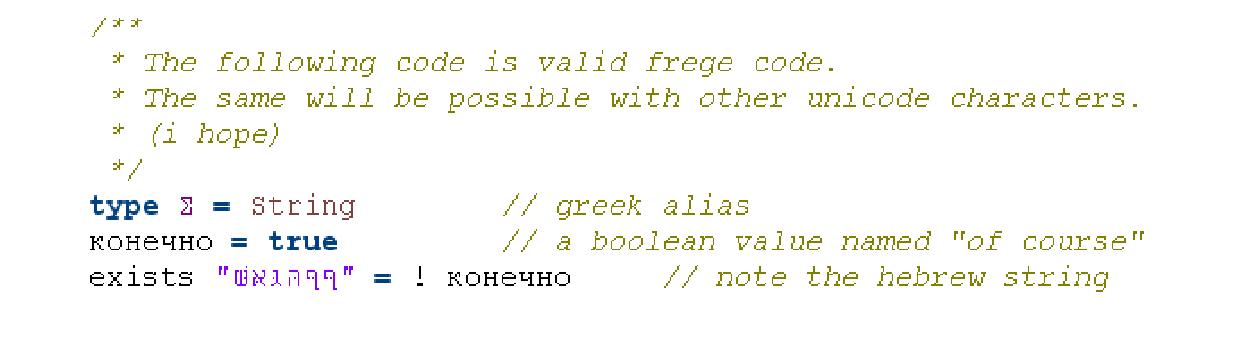
\includegraphics{utfcode}
\caption{\frege{} code with greek, cyrillic and hebrew letters}
\label{utf8}
\end{figure}

\par \frege{} uses the Unicode character set, see \autoref{utf8} for an
example. 
%However, the syntactically relvant characters are drawn from
%the ASCII character set only. The same holds for most names and operators defined in
%the standard libraries. \index{character set!Unicode}

Compilers will support program text stored in files with encodings
that are supported by the \java{} platform. The standard encoding is UTF8.
For detailed information consult the \java{}
API documentation \cite{apidoc}. \index{character!encoding}

While it is possible to compose names and operator symbols from
valid unicode symbols, one should keep in mind that extensive use of
this feature will make the program text
difficult, if not impossible, to understand for members of different
cultural background.

\section{Lexical program structure}

\begin{flushleft}
\rul{program} \some{\nont{line}}\\
\rul{line} \some{\nont{whitespace} \nont{token}} \nont{whitespace}\\
\rul{whitespace} \regex{$\backslash{}$s*}\\
\rul{token} \nont{varid} \oder \nont{conid} \oder \nont{keyword} \oder \nont{qualifier} \oder \nont{parentheses} \oder \nont{specialsym}
\\\hspace{0.5in} \oder \nont{lexop} \oder \nont{literal}
\end{flushleft}

A program is made up of lines.
Source code is broken into lines before tokenization by appropriate
input reading functions that will recognize and strip line separator
characters typical for the underlying operating system. 

With the exception of \hyperref[doccomment]{documentation text} there is no token that would
extend over more than one line.

Each line contains zero or more tokens separated by whitespace. Still
more whitespace can occur before the first token or after the last
token.

Note that the definition of \nont{whitespace} allows for the empty
string of whitespace characters. Consequently, tokens may appear not to
be separated at all.

The possibility of zero length whitespace does not mean that whitespace
may be dismissed altogether. On the contrary, whenever two tokens appear
in sequence where a non empty prefix of the second token might also be a
valid suffix of the first one, nonempty whitespace is required to allow
for unambiguous tokenization. In other words, the tokenization algorithm
will recognize the longest prefix of the remaining characters on the
current line that form a valid token.

Consider the following example:
\example{\par
  a+2\\
  a2\\
  a 2\\
  a\\
 2
}
There are 3 tokens in the first line and one token in the second line.
Since a digit is a valid suffix of an identifier, a space must occur
between a and 2 to obtain two tokens, as shown on the third line.
Another possibility to separate the tokens would be to write them on
different lines, as shown in the last two lines.

\section{Comments} \index{comment}

Comments can appear everywhere whitespace can.

\begin{flushleft}
\rul{comment} \nont{linecomment} \oder{} \nont{blockcomment}\\
\rul{linecomment} \regex{///?.*} \gcom{line comment extends to end of line}\\
\rul{blockcomment} \regex{/$\backslash$*$\backslash$*?}\some{\nont{commenttext}}\regex{$\backslash$*/}\\
\rul{commenttext} \regex{(?s)(.$|$\term{blockcomment})*} \gcom{arbitrary characters or nested comments}
\end{flushleft}

Note that the character sequence making up a \nont{commentttext} may extend over multiple lines
\footnote{This is the only exception to the rule that no token crosses line
boundaries.}.

If some code is commented out using a block comment, then any occurrence of \regex{/*} or \regex{*/} within a string or
within a line comment in that code will interfere with the nested comments. An especially bad idea is to introduce line comments with \regex{//*}. 

\hasdiff{\\
\frege{} adopts the comment syntax of \java{}. But unlike in \java{}, block comments do nest.\\
A user defined operator (see \autoref{operator}) must not start with the characters \texttt{/*} or \texttt{//}.
}

\subsection{Documentation Text} \label{doccomment} \index{comment!documentation}

Block comments starting with \regex{/**} and line comments starting with  \regex{///} are treated as \textit{documentation text}.
Unlike an ordinary comment, a documentation text is a token and hence is not only lexically but also syntactically relevant.

There are only certain places where documentation text may appear, as will be detailed in this section. 
In order not to complicate matters, subsequent sections will not mention documentation text anymore.

A documentation text may appear:
\begin{enumerate}
\item before the \term{package} keyword that starts a package. This will be the documentation for the package.
\item in place of a \hyperref[declarations]{top level declaration} or a declaration in the \term{where} clause of a data, class or instance declaration. It can also appear immediately before such a declaration.
This will be the documentation for the subsequent declared item. 
\item immediately either before or after a \nont{constructor} in a \hyperref[algdcl]{data declaration}. This will be the documentation for that constructor.
\end{enumerate}

For convenience, in cases 1 and 2 a sequence of documentation comments optionally separated by semicolon can be written.
The text of the documentation comments will be concatenated with an interleaving paragraph break.

\example{\\
/// this package is documented\\
/** second paragraph of package doc\\
\\
  3rd paragraph of package doc*/\\
package D where\\
\\
/// this is the list of Fibonacci numbers\\
fib = 1:1:zipWith (+) fib (tail fib)
}

Documentation text will be copied verbatim and it will be available in the binary results of compilation (e.g. \java{} class files), so that documentation processing tools can access it to generate documentation in various formats.


\section{Identifiers and Keywords} \index{identifier} \label {qualified names}

\begin{flushleft}

\rul{qualifier}
\regex{($\backslash$p\{Lu\}($\backslash$d$|$\_$|\backslash$p\{L\})*$\backslash$.)\{1,2\}
}\\

\rul{varid} \regex{$\backslash$p\{Ll\}($\backslash$d$|$\_$|\backslash$p\{L\})*'*}\\

\rul{conid} \regex{$\backslash$p\{Lu\}($\backslash$d$|$\_$|\backslash$p\{L\})*}\\

\rul{qvarid} \nont{qualifier} \nont{varid} \oder{} \nont{varid}\\
\rul{qconid} \nont{qualifier} \nont{conid} \oder{} \nont{conid}\\
\end{flushleft}

These rather complicated regular expressions deserve some further
explanation.

We distinguish lexically between two classes of identifiers.
Names for functions, values and local variables are \nont{varid}s
and start with a lowercase letter.
Names that start with an uppercase letter (\nont{conid})
stand for value constructors,
type constructors, type classes, type alises or name spaces.

Sometimes it is necessary to name an item that is defined in another
package or in the scope of a type or type class. Thus we need qualified
names, defined here as \nont{qvarid} and \nont{qconid}. They are formed
by writing a \nont{qualifier} before a \nont{varid} or \nont{conid}.

A \nont{qualifier} consists of one or two identifiers starting
with an uppercase letter, where each identifier is immediately
followed by a dot. The identifiers denote name spaces, types or type
classes. A \nont{qualifier} like \texttt{Foo.Bar.} is a single
token and thus may not contain spaces.

The syntax ensures that qualifiers will
only be used to form qualified names and will
thus always be followed by either a
\nont{varid} or a \nont{conid}. Hence, we have lexically and syntactically
enforced, that a reference to an item will be one of
the following:

\ex{
$N$.$T$.$v$ \hspace{0.3cm} $N$.$T$.$C$ \\
$T$.$v$  \hspace{0.3cm} $T$.$C$ \hspace{0.3cm}
$N$.$v$  \hspace{0.3cm} $N$.$C$ \hspace{0.3cm} $N$.$T$ \\
$v$ \hspace{0.3cm} $C$ \hspace{0.3cm} $T$
}

where $N$ would be a name space, $T$ a type or class name, $C$ a
data constructor name and $v$ the name of a function or pattern binding.

There are rare cases where it is possible to confuse the dots in the qualifiers with
the special operator \texttt{.} explained later, an example can be found  \hyperref[confusedots]{here}. 
Fortunately, such constructs can be disambiguated with spaces or parentheses.

\note{Unlike in other languages, a \frege{} identifier cannot start with
an underscore.}

\subsubsection{Name Resolution and Scope}

Names appearing in expressions and types are resolved by the following rules, where $N$, $T$ and $C$ stand for \nont{conid}s and $v$ for \nont{varid}s:

\begin{description}
\item [Names of the form $v$] every enclosing lexical scope provided by a \term{let}, lambda expression or case alternative is searched in turn for the name.  If it is found, then it refers to an item defined in a \term{let} expression or a (part of a) pattern in a lambda expression or case alternative. Otherwise, it must be a globally visible item. If $v$ appears in the scope of a data definition, class definition or instance definition and there is a variable or function binding with the name $v$ then it is resolved to mean this binding. Otherwise, it must be a global function or variable binding or a class member.
\item [Names of the form $T$ or $C$] $T$ may appear in type signatures, where it denotes type constructors, type names or class names, either imported ones or ones that are declared in the current package. In expressions and patterns, $C$ denotes a value constructor.
\item[Names of the form $N$.$T$ or $N$.$C$] $N$ must be a name space denoting an imported package, a data type or a class. $T$ must be a class name, type name or $C$ must be a data constructor from this name space. While it is possible, that a type and a data constructor have the same name this does not introduce ambiguities because syntactically either a type name $T$ or a data constructor $C$ can be meant, but not both.

It is also possible that a type name and a name space of an imported package have the same name. In this case, only the name space of the imported package is searched. If one needs to access $C$ in the name space of the type $N.N$ one needs to write a qualified name of the form ($N$.$N$.$C$).
\item[Names of the form $N$.$v$]
$N$ must be name space denoting an imported package, a data type or a class.
$v$ is the name of a function or pattern binding in $N$. Again, if there is a namespace $N$ and a type $T$ and $N = T$, then only $N$ is searched.
\item[Names of the form $N$.$T$.$C$ or $N$.$T$.$v$] denote a function or pattern binding or a data constructor belonging to type or class $T$ from name space $N$.
\end{description}

\subsubsection{Keywords}

Some character sequences that would otherwise be matched by rule \nont{varid} are keywords and will be recognized by the scanner as distinct terminal symbols.

\begin{flushleft}
\label{keyword} \index{keyword}
\term{abstract}: \regex{abstract} \\
%\term{break}: \regex{break} \\
\term{case}: \regex{case} \\
\term{class}: \regex{class|interface}\\
\term{continue}: \regex{continue} \\
\term{data}: \regex{data} \\
\term{derive}: \regex{derive} \\
\term{do}: \regex{do} \\
\term{else}: \regex{else} \\
%\term{extends}: \regex{extends} \\
\term{false}: \regex{false} \\
%\term{for}: \regex{for} \\
\term{if}: \regex{if} \\
\term{import}: \regex{import} \\
\term{in}: \regex{in} \\
\term{infix}: \regex{infix} \\
\term{infixl}: \regex{infixl} \\
\term{infixr}: \regex{infixr} \\
\term{instance}: \regex{instance} \\
\term{let}: \regex{let} \\
\term{native}: \regex{native} \\
\term{of}: \regex{of} \\
\term{package}: \regex{package|module} \\
\term{private}: \regex{private} \\
\term{pure}: \regex{pure} \\
\term{public}: \regex{public} \\
\term{then}: \regex{then} \\
\term{true}: \regex{true} \\
\term{type}: \regex{type} \\
\term{where}: \regex{where} \\
%\term{while}: \regex{while}
\end{flushleft}

\section{Operators} \label{operator} \index{operator!user defined}  \label{fixity} \index{declaration!top level!fixity declaration}

The \frege{} language permits user defined infix operators.
Valid infix operators are sequences of either letters or non word characters that obey the following additional rules:

\begin{enumerate}

\item Certain sequences of 1 or 2 non word characters form
terminal symbols with special syntactic meaning
(rule \nont{specialsym}).
These symbols can not be used as infix operators.

\item Operator symbols may not contain characters used as quotation
marks (rule \nont{quotechar}).

\item Operator symbols may not contain parentheses, brackets or braces (rule \nont{parentheses}).

\end{enumerate}

An infix operator denotes a function or a
value constructor.

Operators may be introduced with a top level infix declaration (rule \nont{fixity}).

\begin{flushleft}
\rul{fixity} \nont{infix} \nont{precedence} \more{\nont{lexop}}
\\
\rul{infix} \term{infix} \oder{} \term{infixl} \oder{} \term{infixr}\\
\rul{precedence} \regex{[123456789]} \oder{} \regex{1[0123456]}\\

\rul{symop}  \regex{$\backslash{}$W+}\\
\rul{wordop} \regex{$\backslash$w+}\\
\rul{infixop} \term{symop} \oder{} \term{wordop}\\
\rul{lexop}  \regex{`}\term{infixop}\regex{`} \oder{} \term{symop}\\
\rul{specialsym} \regex{::} \oder{}
   \regex{->} \oder{}
   \regex{<-} \oder{}
   \regex{$\backslash{}|$} \oder{}
   \regex{=} \oder{} \regex{-} \oder{}
   \regex{!} \oder{} \regex{?} \oder{}
   \regex{,} \oder{} \regex{;} \oder{}
   \regex{$\backslash{}$.} \oder{}
   \regex{$\backslash{}\backslash{}$} \oder{}
   \regex{\_}\\

\rul{parentheses} \regex{$\backslash{}$(} \oder{} \regex{$\backslash{}$)} \oder{} \regex{$\backslash{}$[} \oder{} \regex{$\backslash{}$]} \oder{} \regex{$\backslash{}$\{} \oder{} \regex{$\backslash{}$\}}\\

\rul{quotechar} \regex{["'\#`]}\\
\end{flushleft}

The infix declaration has two purposes:

\begin{itemize}
\item It makes the lexical analyzer recognize operator symbols made up of symbol characters (rule \nont{symop}) in subsequent program text. The lexical analyzer recognizes only operator symbols introduced in an infix declaration and operator symbols from imported packages (see also \autoref{importedops}).

\item It causes the parser to interpret expressions differently based on the operators associativity (left, right or none) and precedence.
Operators with higher precedence bind their operands after operators with lower precedence, so the precedence is to be taken as an ordinal number.
Precedences range from 1 (weakest binding) to 16 (tightest binding).

\end{itemize}

See also the syntax of \emph{binary expressions} in \autoref{binex}, the example in \autoref{exprparse} and the table of predefined operators in \autoref{predefops}.

\subsection{Rules for using backquotes}

Every sequence of characters forming a valid operator symbol that is enclosed in backquotes will be recognized as an operator token. If the operator was not previously introduced through a fixity declaration it will be assumed that it is non-associative and has a precedence of 16.

As outlined above, a \nont{symop} not enclosed in backquotes can only be recognized when there is a fixity declaration or an import that introduces it. Hence, to introduce of a fresh \nont{symop} one must write it within backquotes in the fixity declaration itself.

For \nont{wordop}s matters are different. Like in \haskell{} it is required that one always explicitly indicates when one wants to \textit{use} an identifier as operator. Thus, \nont{wordop}s must always be quoted with backquotes when they are in infix position. However, in the infix declaration all that matters is to announce the character sequence an operator is made of. Thus, backticks are not strictly needed when introducing word operators.

\begin{figure}
%\example{
\begin{code}

infix 12 `==` `!=`       // non associative
infixr 13 `++`           // right associative
infixl 14 div            // left associative word operators, 
infixl 14 `mod`          //  backticks don't matter here
infixr 4 `:`             // right associative
infixr 16 `**`           // ditto, but binds tighter than `:`

a == b != c              // syntax error, set parentheses explicitly
a ++ b ++ c  == d        // (a ++ (b ++ c)) == d
a ** b ** c : d : e      // (a ** (b ** c)) : (d : e)
a `mod` b                // mod a b
f div 2                  // div is not used as operator here
\end{code}
%}
\caption{Parsing of expressions containing operators} \label{exprparse}
\end{figure}

\subsection{Imported operators} \label{importedops}

A package import (see also \autoref{import}) makes all operator symbols introduced in the imported package known to the lexical analyzer. Yet, depending on the import statement, the corresponding function may not be in scope. To access them nevertheless, it is possible to qualify operators:

\begin{flushleft}
\rul{qlexop} \term{qualifier}\regex{?}\term{lexop}
\end{flushleft}

Unlike \nont{qvarid} or \nont{qconid}, \nont{qlexop} is a single token, thus no space may appear between the \nont{qualifier} and the \nont{lexop}.


\hasdiff{
\begin{itemize}
\item fixity is a lexical and syntactical property of certain operator symbols
\item (consequently) fixity declarations are permitted at top level only
\item an operator whose fixity was not declared is taken to be non-associative and to have precedence 16
\item to use an operator \texttt{op} from namespace \texttt{M} one writes \texttt{M.`op`}
\end{itemize}
}

\section{Unary operators}

There are two symbols that may be used as unary operators:

\begin{flushleft}
\rul{unop} \sym{!} \oder{} \sym{?}
%\rul{qunop} \nont{qualifier} \nont{unop} \oder{} \nont{unop}
\end{flushleft}

Unary operators can not be qualified. It is strongly discouraged to use them as names for own functions.

The unary opeartor \sym{!} is the boolean negation function; in patterns it has special meaning that signals  \hyperref[strictpats]{strict patterns}.

The unary operator \sym{?} is currently unassigned and reserved for future use. 

\section{Literals}

Literals are textual representations of values of certain simple types.

\begin{flushleft}
\rul{literal} \nont{boolliteral} \oder{} \nont{numericliteral} \alt{} \nont{charliteral} \oder{} \nont{stringliteral} \oder{} \nont{regexliteral}\\
\rul{numericliteral} \nont{integerliteral} \oder{} \nont{floatliteral}
\end{flushleft}

\hasdiff{Literal syntax is adopted from \java{}. Every literal determines a fixed type.}

\subsection{Boolean Literals}

The boolean values are represented by the keywords \term{true} and \term{false}. Boolean values are of type \texttt{Bool}.

\begin{flushleft}
\rul{boolliteral} \term{true} \oder{} \term{false}
\end{flushleft}

\subsection{Numeric Literals}

The syntax of numeric literals follows closely that of \java{}, except that some exotic form of floating point literals are not supported.
In addition, there are literals for big integers.

Furthermore, for all numeric literals, the syntax of the integral part has been slightly extended: it is possible to separate trailing groups of 3 digits each with an underscore. This enhances legibility greatly with big numbers.

\example{
The literal for the long integer value fifty-two billion four hundred and twennty-five million two hundred and fifty-four thousand five hundred and twenty-four can be written \texttt{52\_425\_254\_524L} or \texttt{52425254524L}.
}

\subsubsection{Integer Literals}

There are literals for values of 3 different integer types: \texttt{Int}, \texttt{Long} and \texttt{Integer}.

\begin{flushleft}
\rul{integerliteral} \nont{intliteral} \oder{} \nont{longliteral} \oder{} \nont{bigintliteral}\\
\rul{intliteral} as defined in \java{}, see section 3.10.1 in \cite{langspec3}\\
\rul{longliteral} as defined in \java{}, see section 3.10.1 in \cite{langspec3}\\
\rul{bigintliteral} \regex{$\backslash$d+(\_$\backslash$d$\backslash$d$\backslash$d)*[nN]} \\
\end{flushleft}

\frege{} adopts the syntax for integer literals from \java{}. An integer literal that would have type \texttt{int} in \java{} has type \texttt{Int} in \frege{}. An integer literal that would have type \texttt{long} in \java{} has type \texttt{Long} in \frege{}.

In addition, a sequence of decimal digits followed by one of the letters \texttt{n} or \texttt{N} (think \emph{natural} number) is a literal of type \texttt{Integer}, the data type of integral numbers of arbitrary size. Note that leading zeroes do not indicate octal numbers as with the other integer literals.


\subsubsection{Floating-Point Literals}

There are literals for values of the \texttt{Float} and \texttt{Double} types. The syntax is a subset of that for \java{} floating point literals as specified in section 3.10.2 of \cite{langspec3}. Not supported are floating point literals that do not start with a digit and hexadecimal floating point literals.

\begin{flushleft}
\rul{floatliteral}
as defined in \java{}, see section 3.10.2 in \cite{langspec3}\\
\hspace{0.5in} except hexadecimal notation and literals\\
\hspace{0.5in} that start with a decimal point
\end{flushleft}

A literal that would have type \texttt{float} in \java{} has type \texttt{Float} in \frege{}. A literal that would have type \texttt{double} in \java{} has type \texttt{Double} in \frege{}.

\subsection{Character and String Literals}

\subsubsection{Character Literals}

Character literals are like \texttt{char} literals in \java{} and have type \texttt{Char}.

\begin{flushleft}
\rul{charliteral}
as defined in \java{}, see section 3.10.4 in \cite{langspec3}\\
\end{flushleft}

\note{Since \frege{} does not preprocess its source texts, a character literal like \texttt{'$\backslash$u89ab'} will not work.}

\subsubsection{String Literals}

String literals are like \texttt{String} literals in \java{} and have type \texttt{String}.

\begin{flushleft}
\rul{stringliteral}
as defined in \java{}, see section 3.10.5 in \cite{langspec3}\\
\end{flushleft}

\note{\java{} programmers: Please observe that the string concatenation operator is \texttt{++} in \frege{}}.

\subsubsection{Literals for Regular Expressions} \label{regexliteral}

The \frege{} language supports regular expressions as a built in data type. Consequently it is possibe to specify regular expressions literally. Such literals denote values of type \texttt{Regex} unless they are not well formed by the rules of the regular expression language. In the latter case, the compiler issues an error message and the program containing the ill formed literal does not compile.

\begin{flushleft}
\rul{regexliteral} \regex{\#($\backslash{}\backslash{}$\#|[\symbol{94}$\backslash{}$\#])*\#}
\end{flushleft}

A regular expression literal is enclosed in number signs and is a sequence of 0 or more characters that are not number signs or number signs escaped with backslashes.

The regular expression language is the one implemented in the \texttt{java.util.regex} package. It is documented along with the class \texttt{java.util.regex.Pattern} in \cite{apidoc}.
The only difference is that the number sign is a special character that signals the end of the regular expression.
If one wants to match a number sign, one must write a backslash followed by a number sign in the regular expression.

\note{A single backslash in a regex literal is the escape character for the regular expression language. Thus, for instance, the literal \regex{\#$\backslash$ba\#} means "the regular expression that matches the letter 'a' after a word boundary" and not "... that matches the backspace character followed by the letter 'a'".
}

It is also possible to construct a string that contains a pattern and compile that to a pattern value. However, regex literals are superior compared to string literals with pattern text
\begin{itemize}
\item because there is one level of backslash-interpretation less, thus one needs to write only half the number of backslashes
\item invalid regex literals are flagged at compile time, not when they are about to be used
\item regex literals will be replaced with references to read only pattern values that are built at program startup time. Thus one can safely use regex literals everywhere without performance penalty due to repeated pattern compilation. This has the added benefit that one can immediately see what the regular expression is and does not have to look it up somewhere else in the program code.
\end{itemize}
The bottom line is: one should use regex literals whenever possible.

\section{Layout} \label{layout}

\frege{} permits the omission of the braces and semicolons by using \emph{layout} to convey the same information.
This allows both layout-sensitive and layout-insensitive styles of coding, which can be freely mixed within one program.
Because layout is not required, \frege{} programs can be straightforwardly produced by other programs.

Informally stated, the braces and semicolons are inserted as follows.
The layout (or "offside") rule takes effect whenever the open brace is omitted after the keyword \term{where}, \term{let}, \term{do}, or \term{of}.
When this happens, the indentation of the next lexeme (whether or not on a new line) is remembered and the omitted open brace is inserted (the whitespace preceding the lexeme may include comments).
For each subsequent line, if it contains only whitespace or is indented more, then the previous item is continued (nothing is inserted);
if it is indented the same amount, then a new item begins (a semicolon is inserted);
and if it is indented less, then the layout list ends (a close brace is inserted).

The layout rule matches only those open braces that it has inserted; an explicit open brace must be matched by an explicit close brace.
Within these explicit open braces, no layout processing is performed for constructs outside the braces, even if a line is indented to the left of an earlier implicit open brace.
See \autoref{layoutrules} for a more precise definition of the layout rules.

\hasdiff{Closing braces are not inserted if an illegal token
is encountered at a point where a closing brace would be legal.}

% $Revision$
% $Id$


\chapter{Expressions} \label{expressions} \index{expression}

In this chapter, we describe the syntax and informal semantics of \frege{} \emph{expressions} and give translations into more basic expressions, where appropriate.
Free variables and constructors used in these translations refer to entities defined by the standard package \texttt{frege.Prelude}.

\section{Terms} \index{expression!term}

\begin{flushleft}
\rul{term} \nont{qvarid} \gcom{variable}
  \alt{} \nont{qconid}  \gcom{constructor}
  \alt{} \nont{qconid}  \sym{\{} \nont{initfields} \sym{\}} \gcom{value construction}
  \alt{} \nont{literal}
  \alt{} \regex{\_} \gcom{a single underscore}
  \alt{} \sym{(} \nont{qlexop} \sym{)}
  \alt{} \sym{(} \nont{qunop} \sym{)}
  \alt{} \nont{section}
  \alt{} \sym{(} \sym{)} \gcom{unit constructor}
  \alt{} \nont{tuple} \gcom{see \autoref{tupleterm}}
  \alt{} \nont{list}  \gcom{see \autoref{listterm}}\\
\rul{initfields} \liste{\nont{initfield}}{,}\\
\rul{initfield} \nont{varid} \opt{\sym{=} \sym{expr}}\\
\end{flushleft}

The most basic expressions are variables, value constructors and literals.
Variables stand for the values they are bound to, often these values are functions.
Likewise, a value constructor may stand for a value or for a function that constructs values depending on other values.

Constructors that were defined with field labels can be applied to a list of field initializations enclosed in braces. 
Exactly the field labels that belong to the constructor must be specified. 
If the expression is omitted, the value of the variable currently in scope that has the same name as the field is used (punning). 
The expression is translated to an ordinary constructor application by reordering the expressions given for the fields so that they appear in the same order as in the constructor definition.

\trans{

\begin{tabular}{lcl}
Con \{ $\cdots$, $a$, $\cdots$ \} & $=$ & Con \{ $\cdots$, $a=a$, $\cdots$ \}\\
Con \{ $a =x_a$, $c =x_c$, $b = x_b$ \} & $=$ & (Con $x_c$ $x_b$ $x_a$)\\
& & if the order of the fields in the\\
& & constructor was $c$, $b$, $a$ \\
\end{tabular}

}

\hasdiff{Values for all fields must be given, it is not allowed to leave out fields.}

Literals stand for the value they represent.

A single underscore is technically a variable, yet can only appear in pattern bindings. There it signals that the corresponding part of a value is not bound.

Sometimes one needs to refer to a function whose name is an operator lexically. Any unary or infix operator may be used as a variable or constructor by enclosing it in parentheses.
Another way to put this is to say that an operator enclosed in parentheses looses its syntactic properties.

\trans{

\begin{tabular}{lcl}
($op$) & $=$ & \emph{the function defined by $op$}, where $op$ is an operator\\
$e_1$ $op$ $e_2$ & $=$ & ($op$) $e_1$ $e_2$, where $op$ is a binary operator\\
$f$ $op$ $e$ & $=$ & $f$ (($op$) $e$), where $op$ is an unary operator\\
\end{tabular}
}

An expression of arbitrary complexity becomes a term syntactically when enclosed in parentheses.

Certain constructs exist to deal with partially applied binary operators and the data types "built in" the language, namely tuples and lists. They all are terms syntactically and are explained in the following subsections.

\subsection{Sections} \index{expression!term!section}

\begin{flushleft}
\rul{section} \sym{(} \nont{binex} \nont{lexop} \sym{)}
 \alt{} \sym{(} \nont{lexop} \nont{expr} \sym{)}
\end{flushleft}

So called \emph{sections} are means of creating functions on the fly by providing the first or second argument to an infix operator (see \autoref{operator}), that is, to a function that takes (at least) two arguments.

For example, the expression $(e < 42)$ denotes one of the values \term{true} or \term{false}, depending on the value of \emph{e}.
We can now abstract out either side of the expression to get two functions:
\begin{enumerate}
\item a function that checks whether its argument is lower than 42
\item a function that checks whether \emph{e} is lower than its argument
\end{enumerate}
Sections permit us to do that syntactically by just leaving out the subexpression we abstract from. We write $( < 42)$ for the first function and $(e <)$ for the second.

\trans{
The following identities hold:
\begin{center}
\begin{tabular}{lcl}
(- e)& $=$ & negate e\\
(`op` e) & $=$ & $\backslash$x \arrow{} x `op` (e)\\
(e -) & $=$ & $\backslash$x \arrow{} e - x\\ 
(e `op`) & $=$ & $\backslash$x \arrow{} e `op` x $=$ (`op`) (e)
\end{tabular}
\end{center}
where \emph{`op`} is a binary operator, \emph{e} is an expression and \emph{x} is a variable that does not occur in \emph{e}
}

The precedence of the operator in a section where the operator comes first is irrelevant. It is so as if the subexpression in the section were always written in parentheses.

However, if the operator stands on the right, its precedence must be taken into account.

For example,the function $(*1+x)$ multiplies its argument with $(1+x)$. But $(1+x*)$ is a syntax error. It must be written like this: $((1+x)*)$.

\subsubsection{Special role of the subtraction/negation operator}

The operator \term{$-$} is treated specially in the grammar. It can act as binary operator, indicating subtraction, or as an unary operator, in which case it indicates negation. 
The token \term{$-$} will \emph{always} refer to the Prelude definition of either subtraction or negation, it is not possible to redefine or qualify it.

Because
$e1-e2$ parses as an infix application of the binary operator \term{$-$}, one must write $e1 (-e2)$ for the alternative
parsing. Similarly, $(-)$ is syntax for $(\backslash x \backslash y$ \arrow{} $x-y)$, 
as with any infix operator, and does not denote
$(\backslash x$ \arrow{} $-x)$ -- one must use \term{negate} for that.

Finally, $(- e)$ is not a section, but an application of prefix negation,
as described above. However, there is a \term{subtract} function defined in the Prelude such
that $(`subtract`$  $e)$ is equivalent to the disallowed section. The expression $(+ (- e))$ can serve the
same purpose.


\subsection{Unit}

The \emph{unit expression} \sym{()} has type () (see \autoref{unittype}); it is the only value of that type.

\subsection{Tuples} \label{tupleterm} \index{expression!term!tuple}

For a discussion of tuple types see \autoref{tupletypes}.

\begin{flushleft}
\rul{tuple} \nont{tupleconstructor} \oder{} \nont{n-tuple} \oder{} \nont{strict-n-tuple}\\
\rul{tupleconstructor} \sym{(,}\some{\sym{,}}\sym{)}\\
\rul{n-tuple} \sym{(}\nont{expr}\sym{,} \liste{\nont{expr}}{\sym{,}}\sym{)}\\
\rul{strict-n-tuple} \sym{(}\nont{expr}\sym{;} \liste{\nont{expr}}{\sym{;}}\sym{)}
\end{flushleft}

Tuples are written $(e_1, ..., e_k)$ where $2\le k \le 26$.
The constructor for an $n$-tuple is denoted by $(,...,)$ where there are $n-1$ commas.
\trans{The following identities hold:\\
\begin{tabular}{lcl}
($e_1$, $e_2$) & $=$ & (,) $e_1$ $e_2$\\
($e_1$, $e_2$, $e_3$)& $=$ & (,,) $e_1$ $e_2$ $e_3$\\
$...$ and so forth up to & & \\
($e_1$, $e_2$, ..., $e_{26}$) & $=$ & (,,,,,,,,,,,,,,,,,,,,,,,,,,) $e_1$ $e_2$ ... $e_{26}$\\
\end{tabular}
}

Tuple construction does not normally cause evaluation of the tuple elements $e_i$. We say that tuple construction is lazy. Sometimes, though, this laziness is not desired. For example, if it is known to the programmer that the tuple elements will be evaluated sooner or later anyway, it can be a good idea to force strict evaluation. For this purpose, replace the commas with semicolons in the tuple construction expression.

\subsection{Lists} \label{listterm} \index{expression!term!list}

Lists are also discussed in \autoref{listtype}.

\begin{flushleft}
\rul{list} \sym{[]}  \gcom{constructor for the empty list}
  \alt{} \bracka{}\liste{\nont{expr}}{\sym{,}}\brackz{}
  \alt{} \bracka{}\nont{expr}\opt{\sym{,} \nont{expr}} \sym{..} \opt{\nont{expr}}\brackz{} \gcom{arithmetic sequence} 
  \alt{} \bracka{}\nont{expr} \sym{$|$} \liste{\nont{dlcqual}}{\sym{,}}\brackz{} \gcom{list comprehension}\\
\rul{dlcqual} \nont{pattern} \term{$\leftarrow$} \nont{expr}
  \alt \nont{expr}
  \alt  \texttt{let} \bracea{} \liste{\nont{decl}}{;} \bracez{}
\end{flushleft}

Lists are written $[e_1, \cdots, e_k]$, where $k>=1$. The list constructor \sym{:} as well as the constructor for the empty list \sym{[]} is considered part of the language syntax and cannot be hidden or redefined.

\trans{The following indentity holds:\\
$[e_1, e_2, \cdots, e_k] = e_1 : (e_2 :( \cdots ( e_k : [] )))$\\
The types of $e_1$ trough $e_k$ must all be the same (call it $t$), and the type of the expression is $[t]$.
}

\subsubsection{Arithmetic Sequences} \index{expression!term!arithmetic sequences} \index{list!arithmetic sequences}
\label{aseq}

The \emph{arithmetic sequence} \bracka{}$e_1$ \opt{, $e_2$} .. \opt{$e_3$}\brackz{} 
denotes a list of values of type $t$, 
where each of the $e_i$ has type $t$, and $t$ is an \hyperref[instance]{instance} of type class \term{Enum}.

\trans{Arithmetic sequences satisfy these identities:\\
\begin{tabular}{lcl}
\bracka{}$e_1$ \sym{..}\brackz{} & = & enumFrom $e_1$\\
\bracka{}$e_1$, $e_2$ \sym{..}\brackz{} & = & enumFromThen $e_1$ $e_2$\\
\bracka{}$e_1$ \sym{..} $e_3$\brackz{} & = & enumFromTo $e_1$ $e_3$\\
\bracka{}$e_1$, $e_2$ \sym{..} $e_3$\brackz{} & = & enumFromThenTo $e_1$ $e_2$ $e_3$\\
\end{tabular}
}

The semantics of arithmetic sequences therefore depends entirely on the \hyperref[instdcl]{instance declaration}
for the type $t$ .

The intended semantics for \emph{enumFrom} is to evaluate to a list that consists of the start element $e_1$, followed by all its successors in ascending order, while \emph{enumFromTo} restricts the sequence of successors up to and including $e_3$. The \emph{enumFromThen} and \emph{enumFromThenTo} functions are variants thereof that produce successive elements whose ordinal values differ by the same amount as the ordinal values of the first two. Hence

\example{enumFrom a = enumFromThen a (succ a)}

It is also possible to create decreasing sequences, by giving an $e_2$ that is smaller than $e_1$.

\subsubsection{List Comprehensions} \index{expression!term!list comprehension} \index{list!comprehension}

List comprehension is a powerful notation to describe lists based on other lists. It has the form $[ e | q_1, \cdots, q_n]$, where $n>=1$ and the qualifiers $q_i$ are either
\begin{itemize}
\item \emph{generators} of the form $p \leftarrow{} e$, where $p$ is a pattern (see \autoref{patterns}) of type $t$ and $e$ is an expression of type $[t]$.
\item \emph{guards}, which are arbitrary expressions of type \texttt{Bool}.
\item \emph{local bindings} \texttt{let} \bracea{} \liste{\nont{decl}}{;} \bracez{}\\
Because list comprehension qualifiers are separated with commas and the keyword \texttt{in} is missing, 
it is not possible to invoke the layout rule by omitting the braces in this case. 
For convenience, a single binding \texttt{let} \bracea{} \nont{decl} \bracez{}
can be written simply \nont{decl}.
\end{itemize}

Such a list comprehension returns the list of elements produced by evaluating $e$ in the successive environments created by the nested, depth-first evaluation of the generators in the qualifier list.
Binding of variables occurs according to the normal pattern matching rules (see \autoref{patternmatch}), and if a match fails then that element of the list is simply skipped over.
Thus:
\example{ [ x $|$ (2, x) $\leftarrow{}$ [(1, 'a'), (2, 'b'), (3, 'c'), (2, 'd')] ]}
yields the list \texttt{['b', 'd']}.

If a qualifier is a guard, it must evaluate to \sym{true} for the previous pattern match to succeed.
As usual, bindings in list comprehensions can shadow those in outer scopes; for example:
\example{[ x $|$ x $\leftarrow{}$ x, x $\leftarrow{}$ x ] = [ z $|$ y $\leftarrow{}$ x, z $\leftarrow{}$ y ]}

\trans{
A list comprehension can be rewritten by the following translation scheme:\\
\begin{tabular}{lcl}
LC [e $|$ Q ] & = & TQ [e $|$ Q ] []\\
TQ [e $|$ ] L & = & \texttt{(e) : L}\\
TQ [e $|$ b, Q] L & = & \texttt{if b then} TQ [e $|$ Q]  L \texttt{else L}\\
TQ [ e $|$ p $\leftarrow$ xs, Q ] L & = &\texttt{let}\\
& &\hspace{1cm}\texttt{h [] = L}\\
& &\hspace{1cm}\texttt{h (p:ys) = }TQ [e $|$ Q] (h ys)\\
& &\hspace{1cm}\texttt{h (\_:ys) = h ys}\\
& &\texttt{in h xs}\\
TQ [ e $|$ \texttt{let \bracea{}} \nont{decls} \texttt{\bracez{}}, Q ] L & = &  
\texttt{let \bracea{}} \nont{decls} \texttt{\bracez{} in} TQ [e $|$ Q] L\\
\end{tabular}\\
where $e$ ranges over expressions, $p$ ranges over patterns, $xs$ ranges over list valued expressions, $b$ ranges over boolean expressions, $Q$ ranges over sequences of qualifiers and \texttt{h} and \texttt{ys} are fresh variables.
}

\paragraph{Example}
Let's translate the following program fragment:
\begin{code}
nums = [1,2,3,4,5,6,7,8,9,10]
squares = [ n*n | n <- nums, n > 4 ]
\end{code}
We have first \ex{nums = 1:2:3:4:5:6:7:8:9:10:[]}
Note that we omitted the parentheses from the translation rule, which is ok since \sym{:} is right associative.

Next we apply translation scheme LC to the list comprehension. This gives us\\
TQ [ n*n $|$ n $\leftarrow$ nums, n $>$ 4 ] []

The TQ scheme has 4 rules that cover all possible forms of a qualifier list. Our qualifier list starts with a generator, thus we have to apply the 3rd rule substituting \texttt{n*n} for $e$, \texttt{n} for $p$ and \texttt{nums} for $xs$. $L$ is the empty list and $Q$ stands for the rest of our qualifier list, which is \texttt{n>4}.
We get

\begin{code}
squares = let
   h1 [] = []
   h1 (n:ys1) = ... // translation of TQ [ n*n | n>4 ] (h1 ys1)
   h1 (_:ys1) = h1 ys1
 in h1 nums
\end{code}

We now have to translate TQ [ n*n $|$ n $>$ 4 ] (h1 ys1) by the second rule, since the qualifier list starts with a guard. We substitute $e$ with \texttt{n*n} as before, $b$ is the guarding expression \texttt{n>4}, $Q$ is empty and $L$ stands for the expression \texttt{(h1 ys1)}.
The result is \ex{
if n>4 then \emph{TQ [ n*n $|$ ] (h1 ys1)} else (h1 ys1)
}
and after translating the last remaining TQ scheme by the first rule, the complete program is

\begin{code}
nums = 1:2:3:4:5:6:7:8:9:10:[]
squares = let
   h1 [] = []
   h1 (n:ys1) = if n>4 then (n*n) : (h1 ys1) else (h1 ys1)
   h1 (_:ys1) = h1 ys1
 in h1 nums
\end{code}

\hasdiff{
In \frege{}, the types \texttt{Double} and \texttt{Float} have no standard instances for \texttt{Enum}, hence floating point arithmetic sequences are not available out of the box.
}

\section{Primary Expression} \label{primexp} \index{expression!primary}

\emph{Primary expressions} are used for invocation of member functions, field selection, field update, array access and array update using a concise notation that will be translated by the compiler. The translations are given below in the usual way.

\begin{flushleft}
\rul{primary} \nont{term}
  \alt \nont{primary} \sym{.} \nont{varid} \gcom{member function application}
  \alt \nont{primary} \sym{.} \nont{lexop} \gcom{member function application}
  \alt \nont{primary} \sym{.} \nont{unop}  \gcom{member function application}
  \alt \nont{qualifier} \sym{\{}\nont{varid} \sym{?}\sym{\}} \gcom{general field existence function}
  \alt \nont{qualifier} \sym{\{}\nont{varid} \sym{=}\sym{\}} \gcom{general field update function}
  \alt \nont{qualifier} \sym{\{}\nont{varid} \sym{<-}\sym{\}} \gcom{general field change function}
  \alt \nont{qualifier} \sym{\{}\liste{\nont{field}}{\sym{,}}\sym{\}} \gcom{update/change values function}
%\alt \nont{tycon} \sym{.} \sym{\{}\nont{varid} \sym{<-} \nont{expr}\sym{\}} \gcom{change value function}
  \alt \nont{primary} \sym{.} \sym{\{}\nont{varid} \sym{?}\sym{\}} \gcom{field existence check}
  \alt \nont{primary} \sym{.} \sym{\{}\nont{varid} \sym{=}\sym{\}} \gcom{update field in value function}
  \alt \nont{primary} \sym{.} \sym{\{}\nont{varid} \sym{<-}\sym{\}} \gcom{change field in value function}
  \alt \nont{primary} \sym{.} \sym{\{}\liste{\nont{field}}{\sym{,}}\sym{\}} \gcom{value update/change}
  \alt \nont{primary} \sym{.} \bracka \nont{expr}\brackz \gcom{array element selection}
% \alt \nont{primary} \sym{.} \bracka \nont{expr} \sym{=} \nont{expr}\brackz \gcom{array update}
% \alt \nont{primary} \sym{.} \bracka \nont{expr} \sym{<-} \nont{expr}\brackz \gcom{destructive array element update}\\
  \alt \texttt{do} \bracea{} \liste{\nont{dlcqual}}{\sym{;}} \bracez{} \gcom{monadic expression}\\
\rul{field} \nont{varid} \sym{=} \nont{expr} \gcom{field update}
  \alt \nont{varid} \sym{<-} \nont{expr} \gcom{field change}
  \alt \nont{varid} \gcom{field update with punning}
\end{flushleft}

The syntax reveals that the \sym{.} works like a left associative operator. This is so that primary expressions can be chained, much like in conventional programming languages. For example \exq{ a.[42].age.negate} could be the negated value associated with the \texttt{age} field of the value in the 43rd element of the array \texttt{a}.

\subsection{Special interpretation of the dot}

The single symbol \sym{.} as syntactic element used to form primary expression will only be recognized if the following conditions all hold:

\begin{itemize}
\item it is not surrounded by white space on both sides (line breaks count as whitespace)
\item the previous token, if any, is not \sym{(}
\item the next token, if any, is not \sym{)}
\end{itemize}

In all other cases, a single \sym{.} will be recognized as \sym{$\bullet$}, which is the function composition operator. 

These rules do not affect recognition of operators that contain one or more dots.

\hasdiff{The single \sym{.} is an overloaded character. If it is enclosed within spaces or if it looks like a section, it will be as if the  function composition operator \sym{$\bullet$}\footnotemark{} had been typed in its place. In all other cases, it is taken as part of a primary expression or a qualified name.

This is to maximize compatibility with \haskell{}, or to make it easy at least to port \haskell{} source code.}
\footnotetext{Unicode \term{U+2022}. Can be produced in Windows with \textsc{Alt+}\texttt{0149} (type number on the numeric keypad), in Linux depending on the input method with \textsc{Compose+}\texttt{.=}}


\subsection{Member function application} \label{memfunapp}
\index{expression!primary!member function application}

This is a convenient notation to apply functions defined locally to a name-space such as a data type or type class. This syntactic form is translated like this:

\trans{\\
\begin{tabular}{lclp{0.6\textwidth}}
$e$.$m$ & $=$ & ($T$.$m$ $e$) & if the expression $e$ has type $t$ and the type constructor of $t$ is $T$ and there exists a function $T$.$m$\\
& $=$ & ($C$.$m$ $e$) & if $m$ is an overloaded function belonging to type class $C$\\
\end{tabular}\\
The conditions will be checked in the order listed here and the first possible translation will be selected. If none of the conditions hold, the compiler flags a type error.
}

Because the compiler creates functions for access to fields in \hyperref[fieldconstructor]{algebraic data types with field labels} that happen to have the same name as the field label, this syntax is most prominent for extraction of field values.

\label{confusedots}For \hyperref[qualified names]{lexical reasons}, when $e$ is a nullary value constructor such as \texttt{Nothing} one cannot write for instance \texttt{Nothing.show} as a shorthand for \texttt{Show.show Nothing}
This is because the lexical analyzer will tokenize this as \nont{qvarid}
and then during name resolution \texttt{Nothing} would be interpreted as name of a type or name space (which would probably fail).
One can avoid this by writing one of \texttt{Nothing . show} (with space before the dot so as to make interpretation as qualified variable impossible) or \texttt{(Nothing).show}

\subsection{Field Existence Test} \label{field existence}
\index{expression!primary!field existence}

The expression $T$.\{$field$\sym{?}\} denotes the function that checks, whether a value $v$ with a type $T u_1 \cdots u_k$  where $k>=0$ was constructed with a \hyperref[fieldconstructor]{data constructor} in whose field list the label $field$ appears.

The expression $v$.\{$field$\sym{?}\} can be used in place of  ($T$.\{$field$\sym{?}\} $v$) if the type of $v$ is already known. The type of $v$ can not be inferred from the former expression, only from the latter one.

\trans{
%\begin{flushleft}
Let it be known that $v$ is of type $t$, and let $t$ be an algebraic data type with constructors $C1$, $C2$ and $C3$. Let label $field$ appear in $C1$ and $C2$. Then the following transformation can be applied:\\
%\end{flushleft}
\begin{tabular}{lclp{0.6\textwidth}}
$T$.\{$field$?\} & $=$ & \sym{$\backslash$}$v$ $\rightarrow$ case $v$ of \{ &\\
& & $C1 \cdots  \rightarrow$ \textbf{true};  & \\
& & $C2 \cdots  \rightarrow$ \textbf{true}; &  \\
& & $C3 \cdots  \rightarrow$ \textbf{false}  \} & \\
$v$.\{$field$?\} & $=$ & ($T$.\{$field$?\} $v$) & -- if $v$ has type $T u_1 \cdots u_k$ \\
\end{tabular}
~\\
The $\cdots$ following the constructors represent the correct number of \_-patterns for the respective constructor.
}

If ($T$.\{$field$\sym{?}\} $v$) returns \term{true}, all field update and access functions for $field$ can be applied to $v$. If it is \term{false}, however, application of any of those functions results in a pattern match failure.

\begin{figure}[hbt]
\example{\tt
\begin{flushleft}
data T = C1 \{name::String, age::Int\}\\
chgName :: T -> String -> T\\
chgName = T.\{name=\}\\
nullifyName :: T -> T\\
nullifyName = T.\{name=""\}\\
age10Factory :: String -> T  -- where age = 10\\
age10Factory = C1 \{name="", age=10\}.\{name=\}\\
incrAge :: Int -> T -> T\\
incrAge n = T.\{age <- (n+)\}
\end{flushleft}
}
\caption{Some primary expressions and their types}
\label{primexprexample}
\end{figure}


\subsection{Value Update and Change by Field Label} \label{fiieldupd}
\index{expression!primary!update by field}

The expression $T$.\{$field$=\} denotes a function that, when applied to two values $v$ and $u$, creates a new value of type $T u_1 \cdots u_k$  (where $k>=0$) that differs from $v$ only in the value for field $field$, which is set to $u$.
This implies that $v$ is also of type $T u_1 \cdots u_k$  (where $k>=0$) and $u$ of the type that was given for label $field$ in the declaration of $T$.

The expression $T$.\{$field$$\leftarrow$\} denotes a function that, when applied to two values $v$ and $g$, creates a new value of type $T u_1 \cdots u_k$  (where $k>=0$) that differs from $v$ only in the value for field $field$, which is set to the result of $g$ applied to the value of $field$ in $v$.
This implies that $v$ is also of type $T u_1 \cdots u_k$  (where $k>=0$) and $g$ of the type ($t \rightarrow t$), where $t$  was the type given for label $field$ in the declaration of $T$.

In both cases, $v$ must have been constructed with a \hyperref[fieldconstructor]{data constructor} in whose field list  the label $field$ appears. Otherwise, the result is undefined, and an attempt to evaluate it will cause a pattern match failure.

\begin{figure}[hbt]
\trans{
Let it be known that $v$ is of type $T$, and let $T$ be an algebraic data type with data constructors $C_1$, $C_2$ and $C_3$. Let label $f$ appear as the first of two fields in $C_1$ and as the second of three fields in $C_2$\footnotemark{}. Then the following transformation is applied:\\
\begin{tabular}{lcp{0.6\textwidth}}
$T$.\{$f$=\} & $=$ & $\backslash v\backslash u \rightarrow$ \textbf{case} $v$ \textbf{of \{} \\
& & \hspace{0.25cm} $C_1$ $a_1$ $a_2 \rightarrow C_1$ $u$ $a_2$;\\
& & \hspace{0.25cm} $C_2$ $a_1$ $a_2$ $a_3 \rightarrow C_2$ $a_1$ $u$ $a_3$ \textbf{\}}\\
$T$.\{$f$$\leftarrow$\} & $=$ & $\backslash v\backslash g \rightarrow$ \textbf{case} $v$ \textbf{of \{} \\
& & \hspace{0.25cm} $C_1$ $a_1$ $a_2 \rightarrow C_1$ ($g$ $a_1$) $a_2$;\\
& & \hspace{0.25cm} $C_2$ $a_1$ $a_2$ $a_3 \rightarrow C_2$ $a_1$ ($g$ $a_2$) $a_3$ \textbf{\}}\\
$v$.\{$f$=\} & $=$ & ($T$.\{$f$=\} $v$)\\
$v$.\{$f$$\leftarrow$\} & $=$ & ($T$.\{$f$$\leftarrow$\} $v$)\\
$T$.\{$f=u$\} & $=$ & (flip $T$.\{$f$=\} $u$) \\
$T$.\{$f\leftarrow g$\} & $=$ & (flip $T$.\{$f\leftarrow$\} $g$) \\
flip $f$ $a$ $b$ & $=$ & $f$ $b$ $a$  -- standard function\\
$v$.\{$f=u$\} & $=$ & ($T$.\{$f$=\} $v$ $u$)\\
$v$.\{$f\leftarrow g$\} & $=$ & ($T$.\{$f\leftarrow$\} $v$ $g$)\\
$v$.\{$f_1=u_1$, & $=$ & $v$.\{$f_1=u_1$\} -- general rules for chained changes/updates\\
\hspace{0.5cm}$f_2\leftarrow u_2$,  &  & \hspace{0.5cm}.\{$f_2\leftarrow u_2$\}\\
\hspace{0.5cm}$f_3=u_3$, $\cdots$\} & & \hspace{0.5cm}.\{$f_3=u_3$\}. $\cdots$\\
$T$.\{$f_1=u_1$, & $=$ & $T$.\{$f_1=u_1$\}\\
\hspace{0.5cm}$f_2\leftarrow u_2$,  &  & \hspace{0.5cm}$\bullet$ $T$.\{$f_2\leftarrow u_2$\}\\
\hspace{0.5cm}$f_3=u_3$, $\cdots$\} & & \hspace{0.5cm}$\bullet$ $T$.\{$f_3=u_3$\} $\bullet$ $\cdots$\\
\end{tabular}    
\par The $a_i$ are auxiliary variables appearing nowhere else in the program. 
\par The identities make it clear that values constructed with $C_3$ cannot be changed or updated, as this constructor has no field $f$.
}
\caption{Translation of change/update primary expressions}
\label{transupdate}
\end{figure}
\footnotetext{
We pick here an arbitrary case for demonstrating purposes. The translation works no matter how many constructors exists, how many of them have a certain field and how many other fields exist. It is precisely the independence of the actual  representation of the values (viz. the type signatures of the constructors) that make the label notation a valuable feature.
}

The update and change functions are created by the compiler whenever an \hyperref[algdcl]{algebraic data type} has a constructor with field labels. They are employed by several forms of the primary expression, whose translation is given in \autoref{transupdate}.

The last 2 rules of  \autoref{transupdate} show that many changes and updates can be mixed in one pair of braces. 

As before, in constructs like $v$.\{$field \cdots$\} where $v$ is an expression, the type of $v$ can not be determined from that construct alone by the type checker. The type of $v$ must be known, either trough a \hyperref[annotation]{type annotation} or the type of $v$ must be unambiguously clear for other reasons.  

\subsection{Array Element Selection} \label{arrayop}
\index{expression!primary!indexed element access}

\todo{write me}


\subsection{Monadic Expression} \index{expression!do}

A \emph{monadic expression} provides syntactic sugar for application of the monadic operators \sym{>>} and \sym{>>=}. Note that the qualifiers share the same syntax with list comprehensions qualifiers but that the translation is quite different.

It is transformed  according to the following rules:

\trans{\\
\begin{tabular}{lcl}
\texttt{do \{} $e$ \texttt{\}} & $=$ & $e$\\
\texttt{do \{} $e$; $q_2$; $\cdots$; $q_i$ \texttt{\}} & $=$ &
$e$ \sym{>>}  \texttt{do \{} $q_2$; $\cdots$; $q_i$ \texttt{\}}\\
\texttt{do \{} $p$ $\leftarrow$ $e$ ; $q_2$; $\cdots$; $q_i$ \texttt{\}} & $=$ &
$e$ \sym{>>=}  ($\backslash p$ \arrow{} \texttt{do \{}  $q_2$; $\cdots$; $q_i$ \texttt{\}}) \\
\texttt{do \{ let \{} $d_1$; $\cdots$; $d_i$ \texttt{\}}; & & \\
\hspace{1.5cm} $q_2$; $\cdots$; $q_i$ \} & $=$ & \texttt{let \{} $d_1$; $\cdots$; $d_i$ \texttt{\}}\\
& & \texttt{in do} \{ $q_2$; $\cdots$; $q_i$ \}\\
\end{tabular}
\par where the $d_i$ range over local declarations, $q_2$; $\cdots$; $q_i$ is a non empty list of arbitrary qualifiers, $e$ stands for an expressions and $p$ for a pattern.
}

The first rule states that the last qualifier in a monadic expression must be an expression.
The remaining rules give the translation for each possible form of the first qualifier.

The type and meaning of the monadic operations are defined in the type class Monad and in the instances for Monad.

\section{Unary operator application}
\index{expression!unary}

\begin{flushleft}
\rul{unary} \nont{primary}
   \alt \nont{qunop} \nont{unary}
\end{flushleft}

The unary operators are just functions with a funny name, however, the precedence of unary operator application is even higher than that of normal function application (see next section). This is so that one can write \texttt{foo !a} and this will be parsed like \texttt{foo (!a)}.


\section{Function application}  \label{funapp} \index{expression!function application}

\begin{flushleft}
\rul{appex} \nont{unary} \alt \nont{appex} \nont{unary}
\end{flushleft}

Function application is the most basic notion in a functional programming language and is written $e_1$ $e_2$.
Application associates to the left, so the parentheses may be omitted in \texttt{(f x) y}.
Because $e_1$ could be a data constructor, partial applications of data constructors are possible.

\example{
The expression \texttt{(,) 1}
denotes a function that, when applied to another expression \texttt{v}, constructs the tuple \texttt{(1,v)}.
}

\paragraph*{Functions are curried}

In \frege{},all functions are considered \emph{curried}; that is, every function $f$ has type $t_1 \rightarrow{} t_2$ for certain types $t_1$ and $t_2$ and thus takes exactly one argument $a$ of type $t_1$ and returns a value of type $t_2$.
Data constructors are just functions, as far as expressions are concerned.
Of course, $t_2$ can itself be a function type, say $t_3 \rightarrow{} t_4$.
In that case the expression $f$ $a$ denotes a value that \emph{is} a function and can be applied to another value $b$ of type $t_3$ immediately, yielding a value of $t_4$. And so forth, ad infinitum.

To be sure, for convenience, the language supports constructs that make it look like there were functios with more than one argument.
\begin{enumerate}
\item Function types can be written $t_1 \rightarrow{} t_2 \rightarrow{} t_3 \rightarrow{} t_4$ since the function type constructor $(\rightarrow)$ is right associative. One may view this as the type of a function that takes 3 arguments.
\item Function definitions can specify more than one argument.
\item Support on the lexical and syntactic level for "binary" operators provide special support for functions that conceptually have 2 arguments.
\item The left associativity of function application itself allows us to write \texttt{f a b c d} and nothing prevents us to think of this as "passing 4 arguments to the function $f$".
\item One can always write its own functions so that they take a tuple of values, which makes function application look very much like in conventional languages, e.g. \texttt{add(1,3)}\footnote{However, this will actually create a tuple on each function call.}
\end{enumerate}

To sum it up, nothing forces a \frege{} programmer to think in terms of single argument functions only.
Yet, it is important to keep in mind that behind the scenes this is all done with single argument functions.
%One consequence of this is, for example, that errors like "function called with too few (or too many) arguments" are impossible to commit in \frege{} programs.

\section{Infix Expressions} \label{binex}
\index{expression!infix or binary}

Infix expressions are applications of infix operators (see \autoref{operator}) written in natural notation. We also speak of  \emph{binary} expressions or operators.

\begin{flushleft}
\rul{binex} \nont{binex$_{1}$}\\
\rul{binex$_{17}$} \nont{appex}\\
\rul{binex$_i$}
        \nont{binex$_i$}     \nont{opleft$_i$}  \nont{binex$_{i+1}$}
   \alt \nont{binex$_{i+1}$} \nont{opright$_i$} \nont{binex$_i$}
   \alt \nont{binex$_{i+1}$} \nont{opnone$_i$}  \nont{binex$_{i+1}$}
   \alt \nont{binex$_{i+1}$}\\
\rul{opleft$_i$}   \nont{lexop$_i$} \gcom{left associative with precedence $i$}\\
\rul{opright$_i$}  \nont{lexop$_i$} \gcom{right associative with precedence $i$}\\
\rul{opnone$_i$} \nont{lexop$_i$} \gcom{non-associative with precedence $i$}\\
\end{flushleft}

The syntax shows that function application has higher precedence than any binary expression, followed by binary expressions of precedence 16 down to 1.

\trans{\\
\begin{tabular}{lcl}
$e_1$ `op` $e_2$ & $=$ & (`op`) ($e_1$) ($e_2$)
\end{tabular}
}

\begin{figure}[bht]
\begin{tabular}{cccl}
Prec. & Assoc. & Operator & Purpose \\
\hline
$16$ & right & \texttt{<\symbol{126}} & function composition\\
$15$ & right & \texttt{**} & exponentiation\\
 & none & \texttt{=\symbol{126} !\symbol{126} ?\symbol{126} /\symbol{126}  \symbol{126} \symbol{126}\symbol{126} \symbol{126}\symbol{126}\symbol{126} } & regular expression matching\\
$14$ & left & \texttt{* / \% `mod`  `div` `rem`} & multiplicative operators\\
$13$ & left & \texttt{+ -} & additive operators\\
 & right & \texttt{++} & string or list concatenation\\
$12$ & left & \texttt{<<} & append to stream\\
& & \texttt{`bshl` `bshr`} & bit shift left/right\\
$11$ & left & \texttt{`band`} & bit-wise and\\
$10$ & left & \texttt{`bor` `bxor`} & bit-wise or/exclusive or\\
$9$ & none & \texttt{< <= > >= } & relational operators\\
$8$ & none & \texttt{<=>} & compare two values\\
$7$ & none & \texttt{== !=} & check for equality/unequality\\
& & \texttt{=== !==} & check for identity\\
$6$ & right & \texttt{\&\&} & logical and\\
$5$ & right & \texttt{||} & logical or\\
$4$ & none  & \texttt{..} & the list of values from .. to\\
& right & \texttt{:} & list constructor\\
$3$ & left & \texttt{>> >>=} & monadic bind operations\\
%$2$ & right & \texttt{:=} & destructive assignment\\
$2$ & right & \texttt{@} & subpattern binding\\
$1$& right & \texttt{\$} & application\\
\end{tabular}
\caption{Predefined Standard Operators} \label{predefops}
\end{figure}

\section{Lambda Expression} \label{lambda}
    \index{expression!lambda}

A lambda expression defines an anonymous function.

\begin{flushleft}
\rul{lambda} \sym{$\backslash$} \nont{pattern} \nont{lambda}
  \alt \sym{$\backslash$} \nont{pattern} \sym{->} \nont{expr}
\end{flushleft}

The syntax of patterns and semantics of pattern matching are explained below, see \autoref{patternmatch}.

A lambda expression $\backslash{}p_1\rightarrow{}\backslash{}p_2 \rightarrow{}\cdots{}\backslash{}p_k \rightarrow{} e$ can be abbreviated\\ $\backslash{}p_1 \backslash{}p_2 \cdots{} \backslash{}p_k \rightarrow{} e$.

A lambda expression $\backslash{}p \rightarrow{} e$ has type $a \rightarrow{} b$ where $a$ is the type of the pattern $p$ and $b$ the type of the expression $e$.

\hasdiff{Each pattern must be introduced with a backslash. Separated this way, even complex patterns don't need parentheses around them, thus something like \texttt{$\backslash$x:\_ $\rightarrow$ x} is valid.}

\trans{
Application of a lambda expression is equivalent to a case expression (see \autoref{caseex})\\
\begin{tabular}{lcl}
($\backslash{}p$ \arrow{} $b$) $e$ & = & \texttt{case} $e$ \texttt{of} $p$ \arrow{} $b$\\
\end{tabular}
\par where $b$ and $e$ are expressions and $p$ is a pattern.
}

\section{Conditional} \label{conditional} \index{expression!conditional}

\begin{flushleft}
\rul{cond} \term{if} \nont{expr} \term{then} \nont{expr} \term{else} \nont{expr}\\
\end{flushleft}

A conditional expression \texttt{if} $e_1$ \texttt{then} $e_2$ \texttt{else} $e_3$ returns $e_2$ if $e_1$ evaluates to \texttt{true}, $e_3$ if $e_1$ is false and is undefined in all other cases.

The condition $e_1$ has type \texttt{Bool} and the possible results have the same type which is also the type of the whole expression.

\section{Let Expressions} \index{expression!let} \label{letexpr}

\begin{flushleft}
\rul{letex} \term{let} \bracea{} \liste{\nont{decl}}{\sym{;}} \bracez{} \term{in} \nont{expr}
\end{flushleft}

Let expressions have the general form
\texttt{let \{} $d_1 ; \cdots{} ; d_n$  \texttt{\} in} $e$,
and introduce a nested,
lexically-scoped, mutually-recursive list of declarations
(let is often called letrec in other languages).
The scope of the declarations is the expression $e$ and the right hand side of the declarations.

Declarations appropriate for use in \texttt{let} expressions are described in \autoref{decl}. The semantics of the nested declarations are described in \autoref{letsemantics}.

Pattern bindings are matched lazily, for example \exq{let (a,b) = (3 `div` 0, 42) in $e$} will not cause an execution time error until \texttt{a} is evaluated.

The value computed by $e$ is also the value of the whole let expression. It follows, that the type of the let expression is the type of $e$.

\section{Case Expressions} \label{caseex} \index{expression!case}

\begin{flushleft}
\rul{casex} \term{case}  \nont{expr} \term{of} \bracea{} \liste{\nont{alt}}{\sym{;}} \bracez{}\\
\rul{alt} \nont{pattern} \sym{->} \nont{expr}
  \alt \nont{pattern} \nont{guarded-exs}
  \alt \nont{alt} \term{where} \bracea{} \liste{\nont{decl}}{\sym{;}} \bracez{}\\
\rul{guarded-exs} \more{\nont{guarded-ex}}\\
\rul{guarded-ex} \sym{$|$} \liste{\nont{lc-qual}}{\sym{,}} \sym{=} \nont{expr}
\end{flushleft}

A case expression has the general form
\begin{center}
\texttt{case} $e$ \texttt{of \{} $p_1$ $match_1$; $\cdots$; $p_n$ $match_n$ \texttt{\}}
\end{center}
where each $match_i$ is of the general form
\begin{center}
\texttt{$|$} $gd_{i_1}$ \texttt{=} $e_{i_1}$
\texttt{$|$} $\cdots$
\texttt{$|$} $gd_{i_m}$ \texttt{=} $e_{i_m}$
\texttt{where \{} $decls_i$ \texttt{\}}
\end{center}
Each alternative $p_i$ $match_i$ consists of a pattern $p_i$ and its matches, $match_i$, which consists of pairs of guards $gd_{i_j}$ and bodies $e_{i_j}$, as well as optional bindings ($decls_i$) that scope over all of the guards and expressions of the alternative.
An alternative of the form
\begin{center}
\nont{pat} \texttt{->} \nont{expr} \texttt{where \{} \nont{decls} \texttt{\}}
\end{center}
is treated as shorthand for:
\begin{center}
\nont{pat} \texttt{$|$ true =} \nont{expr} \texttt{where \{} \nont{decls} \texttt{\}}
\end{center}


A case expression must have at least one alternative and each alternative must have at least one body.
Each body must have the same type, and the type of the whole expression is that type.

A guard is a list of expressions of type \texttt{Bool} or submatches of the form
\begin{center}
\nont{pat} \texttt{$\leftarrow$} \nont{expr}
\end{center}
The expressions will be evaluated in the environment of the case expression extended by the bindings created during the matching of the alternative.
The submatches may themselves create new bindings, these will be in scope for subsequent submatches of the same guard and for the expression associated with that guard.

A guard is matched successful if all expressions yield the result \texttt{true} and all submatches succeed.
A failed match or an expression that evaluates to \texttt{false} causes the next guard to be tried if there is one, otherwise the alternative is not taken.

A case expression is evaluated by pattern matching the expression $e$ against the individual alternatives.
The matches are tried sequentially, from top to bottom.
The first successful match causes evaluation of the expression that is associated with the guard that matched.
If no match succeeds, the result is undefined and the program terminates.
Pattern matching is described in \autoref{patternmatch}, with the formal semantics of case expressions
in \autoref{formalcase}.

\section{Annotated Expression} \label{annex}

\begin{flushleft}
\rul{expr} \nont{topex} \sym{::} \nont{sigma} \alt{} \nont{topex}\\
\rul{topex} \nont{casex} \alt{} \nont{letex} \alt{} \nont{cond} \alt{} \nont{lambda} \alt{} \nont{binex} \\
\end{flushleft}

An expression may be annotated with a type, the notation $e$ :: $t$ means literally \emph{expression} $e$ \emph{has type} $t$. If $e$ has indeed this type, or a more general one, the value $e$ will be computed at the given type, otherwise the compiler will flag an error.

\example{The expression on the right hand side of the function definition\\
foo a b c = a+b-c\\
has type $Num$ $a => a$, i.e. it can have any type that is an instance of type class Num. However, if one writes\\
foo a b c = a+b-c :: Int\\
this restricts the type to Int.
} 


\section{Pattern Matching} \label{patternmatch} \index{pattern} 

Patterns appear in lambda abstractions, function definitions, pattern bindings, list comprehensions, do expressions, and case expressions. However, the first five of these ultimately translate into case expressions, so defining the semantics of pattern matching for case expressions is sufficient.

\subsection{Patterns} \label{patterns} \index{pattern!syntax}

Patterns have this syntax:

\begin{flushleft}
\rul{pattern} \nont{pattern} \sym{::} \nont{sigma} \alt{} \nont{atpattern}\\
\rul{atpattern} \nont{pvar} \sym{@} \nont{atpattern}
  \alt \nont{listpattern}\\
\rul{listpattern} \nont{matcherpattern} \sym{:} \nont{listpattern}
  \alt \nont{matcherpattern}\\
\rul{matcherpattern} \nont{pvar} \sym{\symbol{126}} \nont{regexliteral}
  \alt \nont{pconapp} \\
\rul{pconapp} \nont{pconapp} \nont{strictpattern}
  \alt \nont{strictpattern}\\
\rul{strictpattern} \sym{!} \nont{pterm} \alt{} \nont{pterm} \\
\rul{pterm} \nont{conid}    \gcom{constructor}
    \alt \nont{conid} \sym{\{} \opt{\nont{patternfields}} \sym{\}}
    \alt \nont{pvar}        \gcom{variable, possibly strict}
    \alt \nont{literal}
    \alt \sym{(} \sym{)}    \gcom{unit constructor}
    \alt \sym{[} \sym{]}           \gcom{empty list}
    \alt \sym{[} \liste{\nont{pattern}}{\sym{,}} \sym{]} \gcom{literal lists}
    \alt  \sym{(} \nont{pattern}\sym{,} \liste{\nont{pattern}}{\sym{,}}\sym{)}       \gcom{tuples}
    \alt \sym{(} \nont{pattern} \sym{)}\\    

 \rul{pvar} \nont{varid}   \gcom{variable}
    \alt \regex{\_}           \gcom{anonymous variable}\\

\rul{patternfields} \liste{\nont{varid}\sym{=}\nont{pattern}}{\sym{,}}\\
\end{flushleft}

The pattern syntax is complicated at first sight only. A pattern is, syntactically, just a binary expression (see \autoref{binex}) with the follwoing restrictions:
\begin{itemize}
\item the only infix operators allowed are \sym{@}, \sym{\symbol{126}}, \sym{:} and constructors written in infix notation.
\item only constructor applications are allowed
\item no partial applications are allowed
\item the only unary operator is \sym{!}
%\item the only primary pattern is the record update/record member pattern.
\item pattern tuples and lists are similar in appearance to their expression counterparts, except that they are made up of subpatterns instead of subexpressions. They are just syntactic convenient ways to write constructor applications.
\end{itemize}

In a constructor application pattern, the arity of the constructor must match the number of sub-patterns associated with it; one cannot match against a partially-applied constructor.

In contrast to expressions, constructors with field lists do not have to list all fields. It is even possible to have an empty pattern field list. A constructor with field list is transformed to an ordinary constructor application. The translation inserts anonymous variables for all missing fields.

All patterns must be linear - no variable may appear more than once. For example, this definition is illegal:
\exq{f (x,x) = x -- ILLEGAL; x used twice in pattern}

Patterns of the form $pat$::$type$ assert that the value matched with $pat$ must have type $type$.
Patterns of the form
$var$@$pat$
are called as-patterns, and allow one to use
$var$
as a name for the
value being matched by $pat$. For example, the following function to "sort" a tuple
\exq{$\backslash$(a,b) -> if b<a then (b,a) else (a,b)}
constructs a new value that is equal to the original one in the else clause. To reuse the original value, one could write
\exq{$\backslash$orig@(a,b) -> if b<a then (b,a) else orig}
which is equivalent to
\exq{$\backslash$orig -> case orig of
            (a,b) -> if b<a then (b,a) else orig}

Patterns of the form \_ are wildcards and are useful when some part of a pattern is not referenced on
the right-hand-side. It is as if an identifier not used elsewhere were put in its place.

\subsection{Informal Semantics of Pattern Matching} \index{pattern!matching}

Patterns are matched against values. Attempting to match a pattern can have one of three results: it may \emph{fail}, it may \emph{succeed}, or it may \emph{diverge}.
When the match succeeds, each variable in the pattern will be bound to a value.

Pattern matching proceeds from left to right, and outside to inside, according to the following rules:

\begin{enumerate}
\item Matching a variable $p$ against a value $v$ always succeeds and binds $p$ to $v$.
\item Matching the wildcard pattern \_ against any value succeeds and no binding is done.
\item Matching a pattern of the form $pat$::$t$ against a value $v$ matches $pat$ against $v$.
\item Matching a pattern of the form $pvar$@$pat$ against a value $v$ matches $pat$ against $v$, and if this succeeds, binds $pvar$ to $v$.
\item Matching a pattern $C$ $p_1$ $\cdots$ $p_k$ against a value $v$, where $C$ is a constructor depends on the value:
\begin{itemize}
\item If $v$ is of the form $C$ $v_1$ $\cdots$ $v_k$ ($0\le k\le 26$), the sub-patterns $p_i$ are matched left to right against the components $v_i$; if all matches succeed, the overall match succeeds; the first to fail or diverge causes the overall match to fail or diverge, respectively.
\item If $v$ is of the form $C'$ $v_1$ $\cdots$ $v_n$, where $C'$ is a different constructor to $C$, the match fails.
\item If the value is undefined, the match diverges.
\end{itemize}
Constructors with arity 0 are just a special case without sub-matches.

Constructor application patterns with field lists will have been transformed to ordinary constructor application patterns. Only the named field's subpattern will be matched against the corresponding subvalues. If the pattern field list is empty, just the constructor is checked.
\item Matching a boolean, numeric, string or character literal against a value succeeds if the value equals the value represented by the literal. It diverges if the value is undefined. Otherwise, the match fails.
\item Matching a regular expression literal (see \autoref{regexliteral}) against a value of type \texttt{String} diverges if the value is undefined. It succeeds, if the regular expression matches the string and fails otherwise.
\item If the pattern is of the form $m$\symbol{127}\#$re$\# it will be checked whether the regular expression matches the string as before and when this is the case, the variable $m$ is bound to the matcher employed in the regular expression match. This, in turn, makes it possible to access the matched substring as well as the matched substrings corresponding to any parenthesized groups in the regular expression:
\begin{code}
case "John Smith" of
    m~#(\w+)\s+(\w+)# -> case (m.group 1, m.group 2) of
             (Just a, Just b) -> b ++ ", " ++ a  -- "Smith, John"
\end{code}
\item \label{strictpats} A strict pattern \sym{!}$p$ is matched against a value $v$ by first evaluating $v$ and then matching $p$ against the result. Because evaluation of a value can diverge, matching a strict pattern can diverge in cases  when matching a normal pattern would not. This can change the semantics of a program as the following example shows:
\begin{code}
swap1 (a,b)   = (b,a)
swap2 (!a, b) = (b,a)
ex1 = swap1 (7 `div` 0, 42)   -- yields (42, 7 `div` 0)
ex2 = swap2 (7 `div` 0, 42)   -- diverges
\end{code}

The strict pattern is helpful when the expression can be evaluated efficiently enough to outweigh the imposed cost of laziness:
\example{
\begin{flushleft}
-- drop the first n elements from a list\\
drop n xs = case xs of\\
\hspace{10mm}[] $\rightarrow$ []\\
\hspace{10mm}\_:ys $\rightarrow$ if n $>$ 0 then drop (n-1) ys else xs\\
\end{flushleft}
}
Here, the value $n$ will not be evaluated if the list is empty, thus the application \texttt{drop (7 `div` 0) []} would compute the correct answer (the empty list). But for nonempty lists, $n$ will be evaluated due to the comparison with 0. By making $n$ a strict variable, the function will probably perform better in the vast majority of cases, however, the application above would then cause the program to abort.

\end{enumerate}
\trans{
Matches with regular expressions are translated like this:\\
\begin{tabular}{lcl}
\texttt{case} $v$ \texttt{of} \symbol{35}$rx$\symbol{35} \arrow{} $e$ &
$=$ &
\texttt{case} $v$ \texttt{of} $s$ $|$ $s$ \symbol{126} \#$rx$\# \arrow{}
$e$\\
\texttt{case} $v$ \texttt{of} $m$\symbol{126}\#$rx$\# \arrow{} $e$ &
$=$ &
\texttt{case} $v$ \texttt{of}\\
& &\hspace{0.25cm}$s$ $|$ Just $m$ $\leftarrow$ $s$ =\symbol{126} \#$rx$\# \arrow{} $e$\\
\end{tabular}

where $rx$ stands for the regular expression and $s$ is a fresh variable. (\symbol{126}) is a function defined in the Prelude that checks whether a string is matched by a regular expression.
(=\symbol{126}) is a function defined in the prelude that performs a regular expression match and returns a result of type \texttt{Maybe Matcher}.
}
\subsubsection{Pattern matches that force evaluation}
Some pattern matches force evaluation of the value matched:
\begin{itemize}
\item all literal patterns and $m$\symbol{126}\#$rx$\# need to fully evaluate the value.
\item constructor application patterns for non-product types force evaluation of the value so that the constructor is known.
\item strict patterns forces evaluation of the value in all cases, even if it has a product type. However, subcomponents of the value (if there are any) are not evaluated.
\end{itemize}
\example{
In the example of the drop function above, the constructor patterns for the list argument force the list passed as argument to be evaluated so that the pattern match can see if it is an empty list or a list with at least one element.
}
\subsubsection{Irrefutable patterns}

A pattern is said to be irrefutable, if the match cannot possibly fail or diverge and if the matched value does not have to be evaluated during matching.

\begin{itemize}
%\item Patterns that cause evaluation of the value matched are not irrefutable, because the match can diverge.
\item Non-strict variable and wildcard patterns are irrefutable.
\item $p$::$t$ is irrefutable, if $p$ is
\item $v$@$p$ is irrefutable if $p$ is
\item $C$ $p_0$ $\cdots$ $p_k$ is irrefutable if all subpatterns are irrefutable and if $C$ is the only constructor of the algebraic data type.
\item All other patterns are refutable.
\end{itemize}

Irrefutable patterns are matched lazily. The value of the expression
\example{\textbf{let} swap (a,b)   = (b,a) \textbf{in} swap undefined}
would be $(fst$ $undefined$, $snd$ $undefined)$, that is, binding of the local variables in $swap$ does not extract the values from the argument, nor even evaluation of the argument.

\hasdiff{There exists no syntax to force a pattern to be irrefutable.}

\subsection{Formal Semantics of Case Expressions}

The semantics of all pattern matching constructs other than \texttt{case} expression is defined by giving identities that relate those constrcuts to \texttt{case} expressions. The semantics of \texttt{case} expressions themselves are in turn given as a series of identities, in \autoref{formalcase}. Implementations will behave so that these identities hold; this is not to say that they must use them directly, since that would generate rather inefficient code.

In \autoref{formalcase} $e$, $e'$ and $e_i$ are expressions; $g$ and $g_i$ are guards; $q$ and $q_i$ are qualifiers; $p$ and  $p_i$ are patterns; $v$, $x$ and $x_i$ are variables; $y$ is a fresh variable with a name that differs from all other names in the program; $C$ and $C'$ are algebraic datatype constructors (including tuple, list and record constructors); $r$ is a regular expression literal and $k$ is a boolean, character, string or numeric literal.

\begin{figure}[hbt]
\fbox{
\begin{tabular}{ll}
(a) & \texttt{case} $e$ \texttt{of} \{ $p_1$ $match_1$; $\cdots$; $p_n$ $match_n$ \}\\
&$=$ \texttt{case} $e$ \texttt{of} \{ $p_1$ $match_1$; \_ \arrow{} \texttt{case} $e$ \texttt{of} \{ $p_2$ $match_2$; $\cdots$; $p_n$ $match_n$ \}\}\\
& where each $match_i$ has the form\\
& $|$ $g_{i,1}$ \arrow{} $e_{i,1}$ $|$ $\cdots$ $|$ $g_{i,m}$ \arrow{} $e_{i,m}$ \texttt{where} \{ $decls_i$ \}\\
(b) & \texttt{case} $e$ \texttt{of} \{ $p_1$ $match_1$ \}\\
&$=$ \texttt{case} $e$ \texttt{of} \{ $p_1$ $match_1$; \_ \arrow{} \texttt{error "pattern match failure"} \}\\
(c) &\texttt{case} $e$ \texttt{of} \{\\
&\hspace{0.5cm}$p$ $|$ $g_1$ \arrow{} $e_1$ $|$ $\cdots$ $|$ $g_n$ \arrow{} $e_n$  \texttt{where} \{ $decls$ \};\\
&\hspace{0.5cm}\_ \arrow{} $e'$ \}\\
&$=$  \texttt{case} $e'$ \texttt{of} \{ $y$ \arrow{} \\
&\hspace{0.5cm}\texttt{case} $e$ \texttt{of} \{ $p$ \arrow{} \texttt{let} \{ $decls$ \} \texttt{in}\\
&\hspace{1.0cm}\texttt{case} () \texttt{of} \{ () $|$ $g_1$ \arrow{} $e_1$;\\
&\hspace{3.0cm}\_ \arrow{} $\cdots$ \texttt{case} () \texttt{of} \{ () $|$ $g_n$ \arrow{} $e_n$;\\
&\hspace{7.0cm}\_ \arrow{} $y$; \} $\cdots$ \} \\
&\hspace{2.0cm}\_ \arrow{} $y$; \}\}\\
(d) &\texttt{case} () \texttt{of} \{ () $|$ $q_1$, $\cdots$, $q_n$  \arrow{} $e$; \_ \arrow{} $e'$ \}\\
&$=$  \texttt{case} $e'$ \texttt{of} \{ $y$ \arrow{} \\
&\hspace{0.75cm}\texttt{case} () \texttt{of} \{ () $|$ $q_1$ \arrow{} $\cdots$ \texttt{case} () \texttt{of} \{ () $|$ $q_n$ \arrow{} $e$;\\
&\hspace{7.0cm}\_ \arrow{} $y$; \} $\cdots$ \\
&\hspace{2.0cm}\_ \arrow{} $y$; \}\}\\
(e) &\texttt{case} () \texttt{of} \{ () $|$ $e_0$ \arrow{} $e$  ; \_ \arrow{} $e'$ \}\\
&$=$\texttt{if} $e_0$ \texttt{then} $e$ \texttt{else} $e'$\\
(f) &\texttt{case} () \texttt{of} \{ () $|$ ($e_0$ $\leftarrow$ $p_0$) \arrow{} $e$  ; \_ \arrow{} $e'$ \}\\
&$=$\texttt{case} $e_0$ \texttt{of} \{ $p_0$ \arrow{} $e$; \_ \arrow{} $e'$ \}\\
\end{tabular}
}
\caption{Identities for \texttt{case} expressions}
\label{formalcase}
\end{figure}

Rule (a) matches a general source-language \texttt{case} expression, regardless of whether it actually includes guards - if no guards are written, then \texttt{$|$true} is substituted. Also, the \texttt{where} clause may be missing, this will be equivalent to a \texttt{where} clause with 0 declarations. The rule simplifies a \texttt{case} expression with more than 1 alternatives into a nested \texttt{case} expression where each has at most 2 alternatives.

Rule (b) then supplements a \texttt{case} expression that has exactly one alternative with a catch-all alternative that evaluates to the undefined value. This guarantees that the  \texttt{case} expression evaluates to the undefined value when all matches fail.

From here on, we have to deal with \texttt{case} expressions that have exactly two alternatives, where the second alternative has a simple wildcard pattern without guards and no \texttt{where} clause.

Rule (c) simplifies further by reducing multiple pattern guards to nested  \texttt{case} expressions. The construction \texttt{case () of () \arrow{} $\cdots$} indicates that these  \texttt{case} expressions do no pattern matching, but are just used to look at the guards. They are the only places where guards appear after the translation.

Our  \texttt{case} expressions now have only patterns without guards or a ()-pattern with exactly one guard and no \texttt{where} clauses. A guard may be a list of qualifiers, they are further reduced to nested  \texttt{case} expressions where guards consist of exactly one qualifier in rule (d).

Finally, rules (e) and (f) resolve the single-qualifier-guards. If the guard is a boolean expression, the \texttt{case} expression is transformed into a conditional, otherwise into a \texttt{case} expression that matches the pattern from the qualifier against the expression.

% $Revision$
% $Id$


\chapter{Declarations and Bindings} \label{declarations}
\index{package!declaration} \index{declaration} \index{declaration!package}

In this chapter, we describe the syntax and informal semantics of \frege{} \emph{declarations}.

\begin{flushleft}
\rul{program} \term{package} \nont{packagename} \term{where} \bracea{} \nont{body} \bracez{} \label{packagedcl} \\
%  \alt \term{package} \nont{packagename} \sym{;} \nont{body} \\
\rul{packagename} \nont{qconid}
  \alt \nont{qvarid} \sym{.} \nont{packagename}
  \alt \nont{qconid} \sym{.} \nont{packagename}\\
\rul{body} \nont{topdecl}
  \alt \nont{topdecl} \sym{;} \nont{body}\\
\rul{topdecl} \nont{fixity} \gcom{see \autoref{fixity}}
  \alt \nont{pkgimport}        \gcom{\hyperref[import]{package import}}
  \alt \nont{typedcl}          \gcom{\hyperref[typedcl]{type alias declaration}}
  \alt \nont{datadcl}          \gcom{\hyperref[algdcl]{data type declaration}}
  \alt \nont{classdcl}         \gcom{type class declaration}
  \alt \nont{instdcl}          \gcom{instance declaration}
  \alt \nont{derivedcl}        \gcom{derived instance declaration}
  \alt \nont{decl}\\
\rul{decl} \nont{annotation}    \gcom{type annotation}
  \alt  \nont{binding}          \gcom{function or pattern binding}
  \alt  \nont{nativefun}        \gcom{native function}\\
\rul{decls} \liste{\nont{decl}}{\sym{;}}\\

\end{flushleft}

The \emph{packagename} is a sequence of one or more identifiers where the last identifier starts with an uppercase letter.
The package declaration opens a namespace with a name that equals the last component of the package name.
Each top level item can be accessed with a qualified name that uses the namespace as qualifier, thus in\exq{
package my.fine.pack.with.a.long.name.X where\\
foo = 42\\
bar = let foo = 24 in foo + X.foo
}
\texttt{bar} evaluates to 66.

\index{declaration!top level}

The \emph{body} is a list of top level declarations. It is immaterial in which order the declarations are given.

The declarations in the syntactic category \nont{topdecl} are only allowed at the top level of a \frege{} package, whereas \nont{decl}s can be used either at the top level or in the scope of a data type, class or instance.

For exposition, we divide the declarations into three groups: user defined data types, consisting of type and data declarations; type classes and overloading, consisting of class and instance declarations; and nested declarations, consisting of value bindings and type signatures.

\section{Overview of Types and Classes}
\frege{} uses an polymorphic type system based on the traditional Hindley-Milner type system \cite{ptifart} to provide a static type semantics. The type system supports \emph{type classes} or just \emph{classes} that provide a structured way to introduce \emph{overloaded} functions and values.

A \texttt{class} declaration (\autoref{classdcl}) introduces a new \emph{type class} and the overloaded operations that must be supported by any type that is an instance of that class. An \texttt{instance} declaration (\autoref{instdcl}) declares that a type is an \emph{instance} of a class and includes the definitions of the overloaded operations - called \emph{class methods} - instantiated on the named type. \index{class} \index{instance}

\java{} programmers are familiar with the concept of \emph{interfaces} which serve a similar purpose like \emph{type classes}, but there is a fundamental difference: A \frege{} type class is not a type in its own right like a \java{} interface. Instances of type classes are types, instances of \java{} interfaces are objects.

\subsection{Syntax of Types} \index{type} \index{type!syntax} \label{typesyntax}

The syntax for \frege{} type expressions is given below. Just as data values are built using data constructors, type values are built from \emph{type constructors}. As with data constructors the names of type constructors start with uppercase letters.

The names of type constructors and data constructors will never be confused (by the compiler, that is) as the former only appear in expressions in the form of qualifiers and the latter never appear in types.

\begin{flushleft}
\rul{sigma} \term{forall} \liste{\nont{tyvar}}{} \sym{.} \nont{crho} \gcom{quantified type}
   \alt{} \nont{crho} \\
\rul{crho} \nont{constraints} \sym {=>} \nont{rho}  \gcom{constrained type} \alt{} \nont{rho}\\
\rul{rho} \sym{(} \nont{sigma} \sym{)} \sym{\arrow{}} \nont{rho} \gcom{higher ranked function type} 
  \alt{} \nont{tyapp} \sym{\arrow{}} \nont{rho}                           \gcom{function type}
  \alt{} \nont{tyapp} \\
\rul{constraints} \nont{constraint} 
	\alt{} \sym{(} \liste{\nont{constraint}}{\sym{,}} \sym{)} \label{constraint}\\
\rul{constraint} \nont{classname} \liste{\nont{tvapp}}{} \\
\rul{type} \nont{tyapp} \sym{\arrow{}} \nont{type} \gcom{function type}
  \alt \nont{tyapp}\\
\rul{tyapp} \nont{tyapp} \nont{simpletype}  \gcom{type application}
  \alt \nont{simpletype}\\
\rul{simpletype} \nont{tyvar} \gcom{type variable}
  \alt \nont{tycon}           \gcom{type constructor}
  \alt \sym{(} \nont{type} \sym{)}
  \alt \sym{(} \nont{type} \sym{,} \liste{\nont{type}}{\sym{,}} \sym{)} \gcom{tuple type}
  \alt \sym{\bracka{}} \nont{type} \sym{\brackz{}}  \gcom{list type}\\
\rul{tyvar} \nont{varid} \\
\rul{tvapp} \nont{tyvar} 
\alt{} \sym{(} \liste{\nont{tvapp}}{} \sym{)} \\
\rul{tycon} \nont{qconid}
  \alt \sym{\bracka\brackz}  \gcom{list type constructor}
  \alt \sym{()}              \gcom{unit type constructor}
  \alt \sym{(}\more{\sym{,}}\sym{)} \gcom{tuple type constructors}\\
\rul{classname} \nont{qconid}
\end{flushleft}

The main forms of type expressions are as follows:

\begin{enumerate}
\item Type variables written as identifiers beginning with a lowercase letter.  A type variable can stand for a type or for a partly applied type application.

\item Type constructors. Type constructors are written as identifiers beginning with an uppercase letter. The identifiers may be qualified. Type constructors denote either a user defined data type or a type alias.

Special syntax is provided for the type constructors of the list type, the trivial type and the tuple types.

Type constructors can be constants like \texttt{Int} that denotes the integer type or they can be polymorphic like the list type.
\item Type application. Polymorphic type constructors (or type variables that stand for them) must be applied to type parameters to denote a complete type. For example, the list type constructor requires a type for the elements of the list. The general rule is that only fully applied types must be written. 
\item A parenthesized type ($t$) is identical to the type $t$, but the parenthesis may be required for syntactical reasons.
\end{enumerate}

Special syntax is provided to allow certain type expressions to be written in a more traditional style:

\begin{enumerate}
\item A \emph{function type} has the form $t_1$ \arrow{} $t_2$. Function arrows associate to the right, thus $t_1$ \arrow{} ($t_2$ \arrow{} $t_3$) can be written $t_1$ \arrow{} $t_2$ \arrow{} $t_3$.
\item A \emph{tuple type} has the form ($t_1$, $\cdots$, $t_k$) where $k\ge{}2$, which is equivalent to the type (, $\cdots$,) $t_1$ $\cdots$ $t_k$ where there are $k-1$ commas between the parenthesis.
It denotes the type of $k$-tuples with the first component of type $t_1$, the second component of type $t_2$ and so on.
\item A \emph{list type} has the form $\bracka{}t\brackz{}$, which is equivalent to the type $\bracka{}\brackz{}$ $t$. It denotes the type of lists with elements of the type $t$.
\end{enumerate}

Although the tuple and list types have special syntax, they are not different from user-defined types with equivalent functionality.

\hasdiff{(\arrow{}) is not a type constructor. The only way to write function types is through the infix notation described above.}

Expressions, patterns and types have a consistent syntax. If $t_i$ is the type of expression or pattern $e_i$, then the expressions
($\backslash$ $e_1$ \arrow{} $e_2$),
$\bracka{}e_1\brackz{}$
and ($e_1$, $e_2$) have the types
($t_1$ \arrow{} $t_2$), $\bracka{}t_1\brackz{}$ and ($t_1$, $t_2$),
respectively.

In annotations, annotated expressions and patterns, the type variables in a type expression can be explicitly  quantified (see rule \nont{sigma}). In this case, it is a static error if a type variable that was not quantified appears in the type.
Absent an explicit \term{forall}, all type variables are assumed to be universal quantified. For example, the type expression \texttt{a \arrow{} a} denotes the type $\forall$ $a$.$a$ \arrow{} $a$.
For clarity, however, we'll sometimes write quantification explicitly when discussing the types of \frege{} programs.

More on explicit quantification is explained in the section dealing with \hyperref[higher-rank]{higher rank polymorphism}.

In type annotations as well as in class and instance declarations, the possible types represented by type variables (or applications of type variables) can be \hyperref[constraint]{constrained} to be members of a certain type class. 

\section{User-Defined Data Types} \index{data type}  \index{top level!declaration!data}

In this section, we describe algebraic and native data types (\texttt{data} declaration) and type synonyms (\texttt{type} declaration). These declarations may only appear at the top level of a module.

\subsection{Algebraic Data type Declaration} \index{data type!user defined} \index{data type!algebraic} \label{algdcl}

\begin{flushleft}
\rul{datadcl} \opt{\term{abstract}} \term{data} \nont{conid} \some{\nont{tyvar}} \sym{=} \nont{constructors} \opt{\term{where} \bracea{} \nont{decls} \bracez{}}\\
\rul{constructors} \liste{\nont{constructor}}{\sym{$|$}}\\
\rul{constructor} \opt{\sym{!}} \nont{conid} \some{\nont{simpletype}}\gcom{traditional constructor}
  \alt\  \opt{\sym{!}} \nont{conid} \bracea{} \liste{\nont{varid} ::\nont{type}}{,}\bracez{}\gcom{constructor with fields}\\
\end{flushleft}

An algebraic data type declaration introduces a new type and constructors for making values of that type and has the form:
\begin{quote}
\texttt{data} $T$ $u_1$ $\cdots$ $u_k$ \texttt{=} $K_1$ $t_{11}$ $\cdots$ $t_{1k_1}$ $|$ $\cdots$ $|$ $K_n$ $t_{n1}$ $\cdots$ $t_{nk_n}$
\end{quote}

This declaration introduces a new type constructor $T$ with constituent data constructors $K_1$, $\cdots$, $K_n$ whose types are given by
\begin{quote}
$\forall$ $u_1$ $\cdots$ $u_k$ . $t_{i1}$ \arrow{} $\cdots$ \arrow{} $t_{ik_i}$ \arrow{} $T$ $u_1$ $\cdots$ $u_k$
\end{quote}

The type variables $u_1$ through $u_k$ must be distinct and may appear in the $t_{ij}$; it is a static error for any other type variable to appear in the right hand side.

It is possible to reference the newly introduced type constructor $T$ on the right hand side of its own declaration, which allows to declare recursive types. For example, the following type is like the built-in list type:

\begin{code}
data List a = EmptyList | Cons a (List a)
\end{code}

The declaration can be read "A list of elements of type a is either the empty list or an element of type a "consed" to another list of elements of type a".

There are two special cases for user defined data types:
\begin{description}
\item [product types] are data types with only one constructor. The most prominent product types are tuples.
\item [enumerations] are data types where all constructors are constants, i.e. \exq{
data Colour = Black | Red | Yellow}
%\item [renamed types] are product types where the constructor has exactly one field.
\end{description}

\subsubsection{Visibility of constructors and abstract data types}

\note{to be written}

\subsubsection{Strict or Eager Constructors}

The default behaviour for constructor applications is that the arguments are not evaluated. Evaluation will only take place when a value is deconstructed and a field value so obtained must be evaluated. Hence, operationally, a data structure does not store values but closures.

Sometimes a stricter mode is desired. If one places a \sym{!} before a constructor in a constructor declaration, not only all applications of that constructors will be strict in all arguments, but the data structure will be laid out so that the actual values in native form are stored. This can save time and space, or it can waste time through unnecessary computations. In every case the default lazy semantics change as far as the constructor in question is concerned. 

\subsubsection{Constructors with labeled fields} \label{fieldconstructor}

A different form for constructors is

\begin{quote}
$K_j$ \bracea{} $f_{j1}$ :: $t_{j1}$, $\cdots$, $f_{j{k_j}}$ :: $t_{j{k_j}}$ \bracez{}
\end{quote}

where the $f_ji$ are field labels and the $t_ji$ are the types. 
As before, the type of the constructor is

\begin{quote}
$\forall$ $u_1$ $\cdots$ $u_k$ . $t_{j1}$ \arrow{} $\cdots$ \arrow{} $t_{jk_j}$ \arrow{} $T$ $u_1$ $\cdots$ $u_k$
\end{quote}

Any number of constructors of an algebraic data type can employ the field list syntax. 
Constructors with and without field lists can be mixed.

Every field in one and the same constructor must have a different label, but the same label can appear in a different constructor of the same \term{data} definition. 
All fields with the same label that appear in the same \term{data} definition must have the same type.

The same field label with a possibly different type can appear in constructors of other types. 
This is because field names are only known locally in the type whose constructor introduced them. 
A name given to a field can thus in addition be used for a global variable.

For every field label appearing in an algebraic data type, 
the compiler defines automatically functions that extract a field from a value,
update or change a field in a value
\footnote{This is, of course, nondestructive update, i.e. a new value that differs only in the value for the field is created} 
and check, if the given value has a certain field.

The following box shows how the generated field functions look like. The names of the \emph{upd...}, 
\emph{chg...} and \emph{has...} functions can not be mentioned directly by the programmer, 
as they are picked by the compiler in order to avoid name clashes. 
There exist suitable  \hyperref[primexp]{primary expressions} to obtain and use the functions, though.

\trans{\\
\begin{flushleft}
\textbf{data} T = A $t_{a}$ $|$  B \bracea{}$f_b$ :: $t_{b}$, $f_{bc}$ :: $t_{bc}$ \bracez{} $|$ C \bracea{}$f_{bc}$ :: $t_{bc}$, $f_c$ :: $t_c$\bracez{}\\
\end{flushleft}
translates to
\begin{flushleft}
\textbf{data} T = A $t_a$ $|$  B $t_b$  $t_{bc}$ $|$ C $t_{bc}$ $t_c$ \textbf{where}\\
\hspace{0.3in}// For each of the fields $f_b$, $f_ {bc}$ and $f_c$,\\ 
\hspace{0.3in}// 4 functions will be generated,\\
\hspace{0.3in}// we give here exemplary the ones for $f_{bc}$\\
\hspace{0.3in}$f_{bc}$ $v$ = \textbf{case} $v$ \textbf{of}\\
\hspace{0.5in}B \_ $f$ $\rightarrow$ $f$\\
\hspace{0.5in}C $f$ \_ $\rightarrow$ $f$\\
\hspace{0.3in}upd$f_{bc}$ $v$ $u$ = \textbf{case} $v$ \textbf{of}\\
\hspace{0.5in}B $a$ \_ $\rightarrow$ B $a$ $u$\\
\hspace{0.5in}C \_ $a$ $\rightarrow$ C $u$ $a$\\
\hspace{0.3in}chg$f_{bc}$ $v$ $g$ = \textbf{case} $v$ \textbf{of}\\
\hspace{0.5in}B $a$ $f$ $\rightarrow$ B $a$ ($g$ $f$)\\
\hspace{0.5in}C $f$ $a$ $\rightarrow$ C ($g$ $f$) $a$\\
\hspace{0.3in}has$f_{bc}$ $v$ = \textbf{case} $v$ \textbf{of}\\
\hspace{0.5in}B \_ \_ $\rightarrow$ \textbf{true}\\
\hspace{0.5in}C \_ \_ $\rightarrow$ \textbf{true}\\
\hspace{0.5in}A \_   $\rightarrow$ \textbf{false}
\end{flushleft}
}

\subsubsection{Type Namespaces}

Each declaration of a data type $T$ $u_1$ $\cdots$ $u_k$ with $k \ge 0$ creates also a new namespace. 
This namespace will be populated with the declarations in the optional \term{where} clause of the \term{data} declarations.
Each item $v$ declared in the \term{where} clause of data type $T$ $u_1$ $\cdots$ $u_k$  can be accessed with the qualified name $T$.$v$ and, 
as explained in \autoref{memfunapp}, 
if $e$ is of type $T$ $u_1$ $\cdots$ $u_k$, 
then the expression $e$.$v$ is equivalent to ($T$.$v$ $e$).

\subsubsection{Predefined Algebraic Data Types} \label{predef}

As mentioned elsewhere, \frege{} has some builtin types that are supported with special syntax. Apart from that, they are not different from user defined algebraic datatypes.

\label{unittype}
The unit type $()$ is an enumeration with just one constant, which is also named $()$. The unit type is often the result type of impure functions that exist for their side effects.

\label{tupletypes} \index{tuples}
The tuple types are convenient product types for grouping a fixed number of  values that can have different types. Tuple types with 2 to 26 components are predefined.

\label{listtype} \index{list type}
The list type $\bracka{}a\brackz{}$ is one of the most used types in functional programming. As shown above, a similar type could be defined easily by the user. Although syntactic support as described under \autoref{listterm} would be missing, all expressions and patterns could be translated manually and written down without special syntax.

\hasdiff{
\begin{itemize}
\item Field names live in the namespace that is associated with the constructed type and are not global.
\item Several forms of \hyperref[primexp]{primary expressions} deal with extraction, update and change of fields.
\item Infix notation cannot be used in constructor declarations.
\item No constraints can be given for constructors.
\item There is no \term{deriving} clause. A \hyperref[derivedcl]{derive declaration} can be used instead.
\item Individual fields can not be marked as strict.
\item A data type with exactly one constructor that has exactly one field serves the same purpose as a \term{newtype} declaration.

\end{itemize}
}

\subsection{Native Datatype Declaration} \index{data type} \index{data type!native} \index{data type!user defined} \label{nativedat}

\begin{flushleft}
\rul{datadcl} \term{data} \nont{conid} \nont{tyvar} \sym{=} \term{native} \nont{nativeitem}
	\alt \term{data} \nont{conid} \sym{=} \term{pure native} \nont{nativeitem} \\
\rul{nativeitem} \nont{nativename} \oder{} \nont{stringliteral}
\rul{nativename} \nont{varid}
  \alt \nont{conid}
  \alt \nont{varid} \sym{.} \nont{nativename}
  \alt \nont{conid} \sym{.} \nont{nativename}
\end{flushleft}

A native data type declaration \texttt{data} $T$ $s =$ \texttt{native} $N$ or \texttt{data} $T$ $=$ \texttt{pure native} $N$ introduces a new type constructor $T$ that is associated with the \java{} type $N$. $T$ or ($T$ $s$) is to \frege{} an abstract data type. $N$ may be a primitive java type like \texttt{int} or any java reference type. It is recommended to use fully qualified \java{} names for the latter in order to avoid name clashes in the generated code.

The two syntactic forms help to distinguish between mutable and immutable (pure) data types. Truly immutable objects are rare in \java{}, so in most cases the mutable form will be the appropriate one. A deeper discussion of this matters can be found in \autoref{native interface}.

For convenience, \java{} type names can be specified without quotes, as long as the components are valid \frege{} identifiers. This excludes names starting with underscores or names that contain the \$ sign and also \java{} generic type expressions like \texttt{java.util.List<Integer>}. Such \java{} types must be specified in the form of a string literal.

A \frege{} compiler has no obligation to check the native type name for validity or to know anything about that type, except for the question whether it is a primitive type or a reference type.
This question will be resolved most easily by checking whether the native type name is one of \texttt{boolean}, \texttt{char}, \texttt{byte}, \texttt{short}, \texttt{int}, \texttt{long}, \texttt{float} or \texttt{double}.
If this is the case, the type will be regarded as primitive, otherwise as reference type.
In all other respects, however, the native type is opaque as far as \frege{} is concerned.
The generated code will contain the native type string and this will make the \java{} compiler complain if something is not in order.

Note that \texttt{void} is not a valid native type name since \texttt{void} is not a proper type.

For one and the same native type, more than one native data type declaration can exist. However, the corresponding \frege{} types will be regarded as different types.

Native data types can be used like any other type, for example, they can serve as building blocks for algebraic data types, or be parts of function types. However, since there is no constructor nor any knowledge about the implementation of the type, no pattern matching on values of native data types is possible. Basic operations on the type can be introduced with \hyperref[nativefun]{native function declarations}.

\frege{} borrows all fundamental data types like characters, numbers, booleans and strings from \java{} via native data type declarations. 


\subsection{Type Synonyms} \label{typedcl} \index{declaration!top level!type synonym}

\begin{flushleft}
\rul{typdcl} \term{type} \nont{conid} \some{\nont{tyvar}} \sym{=} \nont{type}
\end{flushleft}

A type synonym has the form
\begin{quote}
\texttt{type} $T$ $u_1$ $\cdots$ $u_k$ = $t$
\end{quote}
where $k\ge 0$ and the $u_i$ are the type variables occuring in the type expression $t$. It is a static error if $t$ contains a type variable not listed on the left hand side among the $u_i$. The $u_i$ must be bare type variables, no constraints are allowed, neither on the left hand side nor on the right hand side.

A type synonym $T_a$ depends on another type synonym $T_b$ if its right hand side mentions $T_b$ or another type synonym $T_c$ that in turn depends on $T_b$.

It is a static error if a type synonym $T$ depends on itself.
This means that cyclic definitions like \exq{
type T a = (a, X a)\\
type X a = T a\\}
are forbidden.

A type expression ($T$ $t_1$ $\cdots$ $t_k$) where $T$ is a type synonym is equivalent to the type expression $t$ of the right hand side of the declaration of $T$ where each variable $u_i$ in $t$ is replaced by the type expression $t_i$. Type synonyms cannot be partially applied in type signatures, it is a static error if during typechecking a type synonym declared with $k$ type variables is found, that is applied to less than $k$ type arguments. However, it is not required that the right hand side of a type synonym declaration is indeed a type; expansion may produce a partially applied type constructor or type synonym:

\begin{code}
type T key value = [(key, value)]
type X = T String

foo :: X Int
foo = [("x", 42)]
\end{code}

In the example above, expansion of type \texttt{X} produces a partially applied type synonym; to form a type one more argument is required.

Type synonyms are most often used to make type expressions more readable and programs more maintenable.

\section{Type Classes and Overloading}
\subsection{Class Declarations} \label{classdcl} \index{class!declaration} \index{declaration!top level!class}

\begin{flushleft}
\rul{classdcl} \term{class} \nont{conid} \opt{\nont{constraints} \sym{=>}} \nont{classvar} \opt{\term{where} \bracea{} \nont{decls} \bracez{}}\\
\rul{classvar}  \nont{varid}
\end{flushleft}

A \emph{class declaration} introduces a new class and the operations (\emph{class methods}) on it. A class declaration has the general form:

\begin{quote}
\texttt{class} $C$ \hspace{0.2cm} ($S_1$ $u$,$\cdots$,$S_k$ $u$)  $=>$ $u$\hspace{0.2cm} \texttt{where} \hspace{0.2cm} \emph{decls}
\end{quote}

This introduces a new class name $C$ with class variabe $u$ and so called superclasses $S_i$.

A class variable stands for potential types that will be instances of the type class. It is also possible that the class variable is higher kinded, i.e. that it is applied to other types in the class operation annotations. The kind of the class variable must be the same in all class operations and in all superclasses.

The $S_i$ denote the superclasses of $C$.
The superclass relation must not be cyclic. If $S$ is a superclass of $C$, then each type that is an instance of $C$ must also be an instance of $S$.

The class declaration introduces new \emph{class methods} in its \emph{decls} part.
The class methods are not only visible in the scope of the class, but also at the top (package) level.
Consequently, a class method can not have the same name as a top level definition or another class method.

A class method declaration is either

\begin{itemize}
\item a new operation introduced with a \hyperref[annotation]{type annotation}. The type given must mention the class variable and the class variable must not be constrained.

Optionally, a definition of the method can be given. The definition serves as a default implementation and will be used in instance definitions that give no instance specific implementation of that method.

A \hyperref[nativefun]{native function} is annotation and definition in one declaration, so this too is allowed. This especially makes sense when one models \java{} inheritance hierarchies with type classes.

\item a definition of one of the class methods of a superclass. There must be no annotation for such methods. The type of the class method will be derived from that of the superclass method by replacing the superclasses' class variable with the current class variable.
\end{itemize}

No other declarations are permitted in the \emph{decls} part of a \texttt{class} declaration.

A \texttt{class} declaration without \texttt{where} clause is equivalent to one with an empty \emph{decls} part.
This can be useful for combining a collection of classes into a larger one that inherits all of the class methods in the original ones.
Nevertheless, even if a type is an instance of all the superclasses, it is not \emph{automatically} an instance of the new class. An instance declaration (with no \texttt{where} clause) is still required to make it one.

The same holds for types that happen to have implementations for all the operations of  a class. That does not make them automatically instances of the class: there is no class membership without an instance declaration.

\paragraph*{Example} We give here a simplified version of some classes declared in the standard Prelude.

\label{classexample}
\begin{code}
class Eq eq where
    (==) :: eq -> eq -> Bool
    (!=) :: eq -> eq -> Bool
    a != b  =  if a == b then false else true

class Ord Eq ord => ord where
    (<)  :: ord -> ord -> Bool
    ...

class Enum Ord enum => enum where
    ord   :: enum -> Int
    from :: Int -> enum
    a == b  =  (ord a) Eq.== (ord b)
    ...
\end{code}

The \texttt{Eq} class introduces two new overloaded operations, with a default implementation for the \texttt{(!=)} method that makes use of the \texttt{(==)} operation. The \texttt{Ord} class is a subclass of \texttt{Eq} and introduces more relational operations. The \texttt{Enum} class is declared as subclass of \texttt{Ord} and this makes it automatically also a subclass of \texttt{Eq}. Therefore, it is possible to give a default implementation for the \texttt{(==)} method. Note that in the definition the reference to \texttt{(==)} needs to be qualified. Without qualification, it would resolve to \texttt{Enum.==} and then the definition could not survive the type check, since it had to be established before that \texttt{Int} was an instance of \texttt{Enum}. But this couldn't be done before the type signature of all declarations in \texttt{Enum} were known and checked.

\subsection{Instance Declarations} \label{instdcl} \index{instance!declaration} \index{declaration!top level!instance}

\begin{flushleft}
\rul{instdcl} \term{instance} \nont{classname}  \opt{\nont{constraints} \sym{=>}} \nont{type} \opt{\term{where} \bracea{} \nont{decls} \bracez{}}
\end{flushleft}

An \emph{instance declaration} introduces an instance of a class. Let
\begin{quote}
\texttt{class} $C$ $u$ \texttt{where \{} \nont{cbody} \texttt{\}}
\end{quote}
be a class declaration.
The general form of the corresponding instance declaration is:
\begin{quote}
\texttt{instance} $C$ ($X_1$ $t_a$,$\cdots$,$X_n$ $t_b$) \sym{=>} $T$ $t_1$ $\cdots$ $t_k$ \texttt{where \{} \nont{decls} \texttt{\}}
\end{quote}
where $k,a,b \ge 0$, $a,b \le k$ and $n \ge 0$. 

If $T$ is a type synonym, the expansion of the type expression must eventually lead to a type application of a type constructor\footnote{... or to a function type, which would constitute a static error, because currently only types that have a type constructor can be instances of type classes}. Otherwise, $T$ itself is already a type constructor. The type expression $T$ $t_1$ $\cdots$ $t_k$ must have the same kind as the class variable of $C$.

An instance declaration may place arbitrary constraints $X_1$ $\cdots$ $X_n$ on all or some of the types represented by the type variables $t_1$ $\cdots$ $t_k$. For example

\example{
instance Eq  (Eq a) \sym{=>} [a] where ...
}

states that for a list type to be an instances of $Eq$, the list elements themselves must be of a type that is an instance of $Eq$. This is another way to say that in order to check list equality, one must be able to check equality on list elements also.

In this example, the instantiated class and the class mentioned in the constraint are the same. This is caused by the logic of relational operations, but is not a language requirement. Any other class could be mentioned as well.

There may be at most one instance per type class and type constructor. Because of this restriction, it is usually a good idea to design the instance as general as possible. The most general case is when the $t_i$ are all distinct type variables.

\example{

\begin{tabular}{ll}
    class C this where ... & \\
    instance C [Int] where ...   & // ok, but quite restrictive\\
    instance C [a]   where ... & // ERROR, [] is already an instance of C\\
    instance C (a,a) where ... & // ok, but restricted\\
    instance C (a,b,c) where ... & // most general instance\\
\end{tabular}

}

\hasdiff{The arguments to a type constructor need not be distinct type variables.

Function types cannot be instances of type classes.

Type synonyms in instance declarations are allowed.

}

\paragraph*{Instance methods}
Instance specific bindings of class methods and not yet implemented superclass methods are searched in the scope of the instantiated type and in the instance declarations $decls$.
It is an error if both sources contain a binding for a class method. It is also an error if none of them contains such a binding unless  there is a default implementation.

Annotations may be given; they will be checked to match the computed type of the instance method.
This type is obtained by substituting the type expression describing the instantiated type for every occurrence of the class variable in the annotation of the class method. In addition, during type check, it will be checked that the definition of the instance method indeed has the computed type, as usual.

It is also possible to implement a class method with a \hyperref[nativefun]{native function}.

If a class method has a default implementation but no instance specific implementation is found, the source code of the default implementation is taken to construct an instance specific implementation.

Each implementation of a class method that comes from the instance declarations or from a default implementation is linked back to the namespace of the instantiated type. This is so that the implementations of class operation \emph{classop} specific for type $T$ can be accessed under the qualified name $T$.\emph{classop}.

It is important to recall that declarations in where clauses of instance or data type declarations live in the scope of the data type or the instance. This has an influence of how unqualified identifiers are resolved. If the name is found in the data or instance context, then it will be resolved to that item and not to the global one. Consider:

\begin{code}
data My a = Val a
instance Show (Show d) => My d where
    show :: Show a => My a -> String 
    show (Val item) = "Val " ++ show item // ERROR
\end{code}

This will produce a rather cryptic error message like
\begin{code}
E X:\dev\frege\S.fr:14: type  `My t3021` is not as polymorphic
                as suggested  in the annotation where just  `a`
                is announced.
E X:\dev\frege\S.fr:14: type error in expression 'item'
        type is  a
        used as  My t3021
\end{code}

Why does it claim that expression \texttt{item}, whose type should be $a$ according to the annotation, is used as \texttt{My t3021}? Because the unqualified variable \texttt{show} resolves to the current instance of \texttt{show} that lives in the instance scope just being defined, and this has a type of \exq{show :: Show d => My d -> String}.
Therefore, the type of \texttt{item} is taken as \texttt{My t3021}. But this implies that the \texttt{show} function just declared would have a type of \exq{show :: Show x => My (My x) -> String}
which is clearly not compatible with the type above, because the annotation is more general than the inferred type. (Note that the very same annotation will be automatically derived from the class definition if it is not given explicitly.)
The remedy is to write either (\texttt{Show.show item}) or just \texttt{item.show} to avoid referring to the \texttt{My.show} function.

\paragraph{Instantiating a Class Hierarchy} with a single instance declaration. It is possible to declare an instance for a subclass and hence to make the instantiated type also an instance of all superclasses without giving explicit instance declarations for the superclasses, provided that
\begin{itemize}
\item the instance declaration contains implementations for the required class methods of the superclasses or
\item the subclass gives default implementations for the superclasses' required methods.
\end{itemize}
For example, the type class \texttt{Ord} is a subclass of \texttt{Eq}, but has a default implementation for \texttt{(Eq.==)}.
Class \texttt{Eq} itself has a default implementation for \texttt{(Eq.!=)}.
Thus it is possible to declare  \texttt{Ord} instances without caring about the \texttt{Eq} methods.


\subsection{Derived Instances} \label{derivedcl}

For the Prelude classes \texttt{Eq}, \texttt{Ord}, \texttt{Enum}, \texttt{Bounded} and \texttt{Show} it is possible to \emph{derive} instances automatically.

\begin{flushleft}
\rul{derivedcl} \term{derive}  \nont{classname}  \opt{\nont{constraints} \sym{=>}} \nont{type} 
\end{flushleft}

Derived instances provide convenient commonly-used operations for user-defined data types.
For example, derived instances for data types in the class \texttt{Eq} define the operations \texttt{==} and \texttt{!=}, freeing the programmer from the need to define them. The precise details of how
the derived instances are generated for each of these classes are given below,
including a specification of when such derived instances are possible.

\trans{
A valid \texttt{derive} declaration is translated like this:\\
\begin{tabular}{ll}
\textbf{derive} & $C$ ($X_1$ $t_a$,$\cdots$, $X_n$ $t_b$) \sym{=>} $T$ $t_1$ $\cdots$ $t_k$ $=$ \\
& \textbf{instance} $C$ ($X_1$ $t_a$,$\cdots$, $X_n$ $t_b$) \sym{=>} $T$ $t_1$ $\cdots$ $t_k$ \\
& \hspace{1cm}\textbf{where \{} $decls_C$ \textbf{\}}\\
\textbf{derive} & $C$ $T$ $t_1$ $\cdots$ $t_k$ $=$ \\
& \textbf{instance} $C$ ($C$ $t_1$,$\cdots$, $C$ $t_k$) \sym{=>} $T$ $t_1$ $\cdots$ $t_k$ \\
& \hspace{1cm}\textbf{where \{} $decls_C$ \textbf{\}}\\
\end{tabular}
\par where $decls_C$ are compiler generated declarations whose concrete content depends on $C$ and the structure of $T$  $t_1$ $\cdots$ $t_k$.
}

As with instance declarations, it is possible to specify constraints in derive declarations. The constraints so given must contain the set of constraints  ($C$ $t_1$,$\cdots$, $C$ $t_k$) where $C$ is the derived class and  the $t_i$ are the type variables of the instantiated type. If, however, no constraints at all are given, the constraints needed will be silently supplied by the compiler.

\subsubsection{Derived Instances for Eq}

Instances of \texttt{Eq} are types whose values can be compared for equality. \texttt{Eq} instances can be derived for all algebraic data types.

\trans{
Let $P$ be a $n$-ary $(n \ge 0)$ type constructor for a product type with $k$-ary $(k \ge 0)$ data constructor $C$:
\begin{flushleft}
\textbf{data} $P$ $u_1$ $\cdots$ $u_n$ = $C$ $ct_1$ $\cdots$ $ct_k$\\
\hspace{1cm}Then\\
\textbf{derive} \texttt{Eq} ($P$ $t_1$ $\cdots$ $t_n$)\\
\hspace{1cm}is equivalent to:\\
\textbf{instance} \texttt{Eq}  ($Eq$ $t_1$, $\cdots$, $Eq$ $t_n$) \sym{=>} ($P$ $t_1$ $\cdots$ $t_n$) \textbf{where}\\
\hspace{0.3cm}$C$ $a_1$ $\cdots$ $a_k$ \texttt{==} $C$ $b_1$ $\cdots$ $b_k$ \texttt{=}\\
\hspace{0.6cm}\textbf{true} \texttt{\&\&} $a_1$ \texttt{Eq.==} $b_1$ \texttt{\&\&} $\cdots$ \texttt{\&\&} $a_k$ \texttt{Eq.==} $b_k$\\
\end{flushleft}
}

The generated expression returns \textbf{true} if all subcomponents of the left operand are pairwise equal with the corresponding subcomponents of the right operand, otherwise the result is  \textbf{false}.

Note that the special case $k=0$ is trivial: such a type has only one value $C$ and the derived \texttt{==} returns always \textbf{true}.

The case gets only marginally more complex with sum types.
\trans{
Let $S$ be a $n$-ary $(n \ge 0)$ type constructor for a sum type with $m$  $(m \ge 2)$ data constructors $C_1, \cdots, C_m$ and arities $k_1, \cdots, k_m$:
\begin{flushleft}
\textbf{data} $S$ $u_1$ $\cdots$ $u_n$ = $C_1$ $ct_{1_1}$ $\cdots$ $ct_{k_1}$ $| \cdots |$ $C_m$ $ct_{m_1}$ $\cdots$ $ct_{k_m}$\\
\hspace{1cm}Then\\
\textbf{derive} \texttt{Eq} ($S$ $t_1$ $\cdots$ $t_n$)\\
\hspace{1cm}is equivalent to:\\
\textbf{instance} \texttt{Eq} ($Eq$ $t_1$, $\cdots$, $Eq$ $t_n$) \sym{=>} ($S$ $t_1$ $\cdots$ $t_n$) \textbf{where}\\
\hspace{0.33cm}$a$ \texttt{==} $b$ \texttt{=} \textbf{case} $(a, b)$ \textbf{of}\\
\hspace{0.66cm}$(C_1 a_1 \cdots a_{k_1}, C_1 b_1 \cdots b_{k_1})$\\
\hspace{2cm}$\rightarrow$ \textbf{true}  \texttt{\&\&} $a_1$\texttt{.==} $b_1$ \texttt{\&\&} $\cdots$ \texttt{\&\&} $a_{k_1}$\texttt{.==} $b_{k_1}$\\
\hspace{0.66cm}$\cdots$\\
\hspace{0.66cm}$(C_m a_1 \cdots a_{k_m}, C_m b_1 \cdots b_{k_m})$\\
\hspace{2cm}$\rightarrow$ \textbf{true} \texttt{\&\&} $a_1$\texttt{.==} $b_1$ \texttt{\&\&} $\cdots$ \texttt{\&\&} $a_{k_m}$\texttt{.==} $b_{k_m}$\\
\hspace{0.66cm}\_ $\rightarrow$ \textbf{false}
\end{flushleft}
}

The expression $a$ \texttt{==} $b$ evaluates to \textbf{true} if both $a$ and $b$ were constrcuted with the same data constructor and their corresponding subcomponents are pairwise equal.

\subsubsection{Derived Instances for Ord}
The \texttt{Ord} class is used for totally ordered datatypes. It is a subclass of \texttt{Eq} and inherits the operations \texttt{==} and \texttt{!=}. It defines one new operation \texttt{<=>} that must be implemented by all instances, and operations \texttt{<}, \texttt{<=}, \texttt{>}, \texttt{>=}, \texttt{max} and \texttt{min} in terms of \texttt{<=>}.

The compare function \texttt{<=>} compares two values and returns a result of type \texttt{Ordering}, which is defined as
\begin{code}
    data Ordering = Lt | Eq | Gt
\end{code}

Instances of \texttt{Ord} can be derived for all algebraic data types. Derived instances for sum types make use of the Prelude function
\begin{quote}
\texttt{constructor} :: $any \rightarrow$ \texttt{Int}
\end{quote}
which returns the index of the constructor for algebraic data types.\footnote{The constructors are numbered starting from 0 in the order they appear in the \hyperref[datadcl]{data declaration}.}

\trans{
Let $P$ be a $n$-ary $(n \ge 0)$ type constructor for a product type with $k$-ary $(k \ge 1)$ data constructor $C$:
\begin{flushleft}
\textbf{data} $P$ $u_1$ $\cdots$ $u_n$ = $C$ $ct_1$ $\cdots$ $ct_k$\\
\hspace{1cm}Then\\
\textbf{derive} \texttt{Ord} ($P$ $t_1$ $\cdots$ $t_n$)\\
\hspace{1cm}is equivalent to:\\
\textbf{instance} \texttt{Ord} ($Ord$ $t_1$, $\cdots$, $Ord$ $t_n$) \sym{=>} ($P$ $t_1$ $\cdots$ $t_n$) \textbf{where}\\
\hspace{0.33cm}$(C a_1 \cdots a_k)$ \texttt{<=>} $(C b_1 \cdots b_k)$ \texttt{=} \textbf{case} $a_1$\texttt{.<=>} $b_1$ \textbf{of}\\
\hspace{0.66cm}\texttt{Eq} $\rightarrow$\\
\hspace{1cm}$\cdots$\\
\hspace{1.33cm}\textbf{case} $a_{k-1}$\texttt{.<=>} $a_{k-1}$ \textbf{of}\\
\hspace{1.66cm}\texttt{Eq} $\rightarrow$ $a_k$\texttt{.<=>} $b_k$\\
\hspace{1.66cm}$r_{k-1}$ $\rightarrow$ $r_{k-1}$\\
\hspace{1cm}$\cdots$\\
\hspace{0.66cm}$r_1$ $\rightarrow$ $r_1$\\
\end{flushleft}
}
The generated expression compares the components $a_i$, $b_i$ from 1 to $k-1$; the first result $r_i$ that does not signify equality is the result of the overall comparison. Otherwise, if all component pairs up to ${k-1}$ compare equal, the result is the ordering of the last component pair, $a_k$\texttt{.<=>} $b_k$.

The translation does not handle the case of the trivial product type. Such a type will have an implementation of \texttt{<=>} that always returns \texttt{Ordering.Eq}.

It follows the translation for sum types.

\trans{
Let $S$ be a $n$-ary $(n \ge 0)$ type constructor for a sum type with $m$  $(m \ge 2)$ data constructors $C_1, \cdots, C_m$ and arities $k_1, \cdots, k_m$:
\begin{flushleft}
\textbf{data} $S$ $u_1$ $\cdots$ $u_n$ = $C_1$ $ct_{1_1}$ $\cdots$ $ct_{k_1}$ $| \cdots |$ $C_m$ $ct_{m_1}$ $\cdots$ $ct_{k_m}$\\
\hspace{1cm}Then\\
\textbf{derive} \texttt{Ord} ($S$ $t_1$ $\cdots$ $t_n$)\\
\hspace{1cm}is equivalent to:\\
\textbf{instance} \texttt{Ord} ($Ord$ $t_1$, $\cdots$, $Ord$ $t_n$) \sym{=>} ($S$ $t_1$ $\cdots$ $t_n$) \textbf{where}\\
\hspace{0.33cm}$a$ \texttt{<=>} $b$ \texttt{=} \textbf{case} \texttt{constructor} $a$ \texttt{Int.<=>} \texttt{constructor} $b$ \textbf{of}\\
\hspace{0.66cm}\texttt{Eq} $\rightarrow$ \textbf{case} $(a,b)$ \textbf{of}\\
\hspace{1cm}$alt_1$\\
\hspace{1cm}$\cdots$\\
\hspace{1cm}$alt_m$\\
\hspace{0.66cm}$r_0$ $\rightarrow$ $r_0$
\end{flushleft}
where each of the alternatives $alt_i$ has a form that depends on the arity of the constructor $C_i$:
\begin{flushleft}
\hspace{0.3cm}$(C_i, C_i) \rightarrow$ \texttt{Eq}\hspace{\fill}for nullary $C_i$\\
\hspace{0.3cm}$(C_i a_1, C_i b_1) \rightarrow a_1$\texttt{.<=>} $b_1$ \hspace{\fill}for unary $C_i$\\
\hspace{0.3cm}$(C_i a_1 \cdots a_{k_i}, C_i b_1 \cdots b_{k_i}) \rightarrow$ \hspace{\fill}for $C_i$ with arity $k_i \ge 2$\\
\hspace{1cm}$(a_1, \cdots, a_{k_i})$\texttt{.<=>} $(b_1, \cdots, b_{k_i})$
\end{flushleft}
}
The comparison first sorts out the cases where the constructors are not the same; the result in such a case is the ordering of the constructors. The remaining $m$ cases compare nullary constructors equal to themselves, values with unary constructors compare just like the components compare and values with constructors of higher arity compare like the tuples constructed from their components would compare when $k_i$-ary tuples had a derived instance of \texttt{Ord}.

\subsubsection{Derived Instances for Enum}

The \texttt{Enum} class is good for algebraic datatypes that have only nullary constructors.
It provides conversion from and to \texttt{Int} values, successor and predecessor functions and the operation ($a$ \texttt{..} $b$) that constructs a list of all values $e$ where $a \le e \le b$. \texttt{Enum} is a subclass of \texttt{Ord}.

A trivial type can be an instance of \texttt{Enum}.
\trans{
Let $T$ be a trivial type:
\begin{flushleft}
\textbf{data} $T$ = $C$\\
\hspace{1cm}Then\\
\textbf{derive} \texttt{Enum} $T$\\
\hspace{1cm}is equivalent to:\\
\textbf{instance} \texttt{Enum} $T$ \textbf{where}\\
\hspace{0.5cm}ord $C$ = 0; from 0  = $C$\\
\end{flushleft}
}

Product types with arity $k>0$ cannot be instances of \texttt{Enum}. It remains to show the translation for those sum types that can be instances of \texttt{Enum}.

\trans{
Let $S$ be a sum type with $m$ $(m \ge 2)$ nullary constructors:
\begin{flushleft}
\textbf{data} $S$ = $C_1 | \cdots | C_m$\\
\hspace{1cm}Then\\
\textbf{derive} \texttt{Enum} $S$\\
\hspace{1cm}is equivalent to:\\
\textbf{instance} \texttt{Enum} $S$ \textbf{where}\\
%\hspace{0.5cm}minval = $C_1$; maxval = $C_m$\\
\hspace{0.5cm}ord $e$ = \textbf{case} $e$ \textbf{of}\\
\hspace{1.0cm}$C_1 \rightarrow$ 0\\
\hspace{1.0cm}$\cdots$\\
\hspace{1.0cm}$C_m \rightarrow$ $m-1$\\
\hspace{0.5cm}from $i$  = \textbf{case} $i$ \textbf{of}\\
\hspace{1.0cm}0 $\rightarrow C_1$\\
\hspace{1.0cm}$\cdots$\\
\hspace{1.0cm}$m-1$ $\rightarrow C_m$\\
\end{flushleft}
}
Note that the construct $m-1$ will be substituted by the appropriate integer constant. The application ($S$\texttt{.from} $i$) is undefined for $(i<0)$ or $(i \ge m)$. For all $C_i$ it is the case that $S$\texttt{.from} $C_i$\texttt{.ord ==} $C_i$

\subsubsection{Derived instances for Bounded}

This type class defines two per type constants \emph{minBound} and \emph{maxBound} and can be derived for enumeration types.
\trans{
Let $S$ be a sum type with $m$ $(m \ge 2)$ nullary constructors:
\begin{flushleft}
\textbf{data} $S$ = $C_1 | \cdots | C_m$\\
\hspace{1cm}Then\\
\textbf{derive} \texttt{Bounded} $S$\\
\hspace{1cm}is equivalent to:\\
\textbf{instance} \texttt{Bounded} $S$ \textbf{where}\\
\hspace{0.5cm}minBound = $C_1$\\
\hspace{0.5cm}maxBound = $C_m$\\
\end{flushleft}
}

\subsubsection{Derived instances for Show}

The type class \texttt{Show} is for types whose values can be represented as character strings. It can be derived for any algebraic data type.

\trans{
Let $S$ be a $n$-ary $(n \ge 0)$ type constructor for a type with $m$  $(m \ge 1)$ data constructors $C_1, \cdots, C_m$ and arities $k_1, \cdots, k_m$:
\begin{flushleft}
\textbf{data} $S$ $u_1$ $\cdots$ $u_n$ = $C_1$ $ct_{1_1}$ $\cdots$ $ct_{k_1}$ $| \cdots |$ $C_m$ $ct_{m_1}$ $\cdots$ $ct_{k_m}$\\
\hspace{1cm}Then\\
\textbf{derive} \texttt{Show} ($S$ $t_1$ $\cdots$ $t_n$)\\
\hspace{1cm}is equivalent to:\\
\textbf{instance} \texttt{Show} ($Show$ $t_1$, $\cdots$, $Show$ $t_n$) \sym{=>} ($S$ $t_1$ $\cdots$ $t_n$) \textbf{where}\\
\hspace{0.5cm}\texttt{show v =} \textbf{case} \texttt{v} \textbf{of}\\
\hspace{1cm}$C_1 a_1 \cdots a_{k_1} \rightarrow$ \texttt{"}$C_i$\texttt{" ++ " "}\\
\hspace{2cm}\texttt{ ++} $a_1$\texttt{.showsub ++} $\cdots$ \texttt{" " ++} $a_k$ \texttt{.showsub}\\
\hspace{1cm}$\cdots$\\
\hspace{1cm}$C_m a_1 \cdots a_{k_m} \rightarrow \cdots$\\
\hspace{0.5cm}\texttt{showsub} $C_i$ \texttt{=} \texttt{"}$C_i$\texttt{"}\hspace{\fill}for each $i$ where $k_i=0$\\
\hspace{0.5cm}\texttt{showsub} $C_i a_1 \cdots a_{k_i}$ \texttt{=} \hspace{\fill}for each $i$ where $k_i>0$\\
\hspace{2cm}\texttt{"(" ++ show (} $C_i a_1 \cdots a_{k_i}$\texttt{) ++ ")"}
\end{flushleft}
}

The derived \texttt{show} functions create a textual representation of a value that will be syntactically reminiscent of a  constructor application if the \texttt{Show} instances of the subcomponents behave likewise. The \texttt{showsub} function shows the value enclosed in parenthesis if it is more complex than just a nullary constructor.

The translation above is equally valid for product and sum types. Types that enjoy special syntactic support (list types, tuples,  and the unit type) have also special \texttt{Show} instances whose translation is omitted for brevity. Suffice it to say that these instances will reproduce the familiar textual representations, i.e. the expression \texttt{show (1,2)} will produce \texttt{"(1, 2)"} and not \texttt{"(,) 1 2"}.

\subsection{Ambiguous Types}

A problem inherent with overloading is the possibility of an \emph{ambiguous type}.
For example, using the \emph{from} and \emph{ord} functions from the \emph{Enum} class introduced in the last section, then the following declaration
\exq{amb x = if ord (from 1) == 1 then x else x+x}
causes the type inference algorithm to attribute the type
\exq{(Enum b,Num a) \sym{=>} a $\rightarrow$ a}
to \emph{amb}. If such type were allowed, it would never be possible to decide at which type to instantiate type variable $b$ which is totally unrelated to type variable $a$ which stands for the argument's type. Therefore, such types are considered ill-typed and programs containing them are rejected.

We say that an expression has an ambiguous type if, in its type 
\exq{\textbf{forall} $u_1$, $\cdots$, $u_k$ \sym{.} $cx$ \sym{=>}  $t$ }
there is a type variable $u_j$ that occurs in $cx$ but not in $t$.

Ambiguous types can only be circumvented by input from the user. One way is through the use of expression
type-signatures as described in \autoref{annex}. Our example could be rewritten as follows:
\exq{amb x = if ord (from 1 :: Bool) == 1 then x else x+x}

\section{Nested Declarations} \label{decl}

The declarations described here can appear at the top level or in the scope of a class  declaration, instance declaration or datatype declaration. With the exception of the \hyperref[nativefun]{native function declaration} they can also appear in a \hyperref[letexpr]{\texttt{let} expression}. In fact, this are the only declarations allowed in \texttt{let} expressions and \texttt{where} clauses that are part of expressions. (Such \texttt{where} clauses will be transformed to \texttt{let} expressions ulitmatively.)

\begin{flushleft}
\rul{decl} \nont{annotation} \gcom{Type Annotation}
  \alt \nont{binding}        \gcom{Function or Pattern Binding}
  \alt \nont{nativefun}      \gcom{Native Function Declaration}
\end{flushleft}

\subsection{Type Annotations} \label{annotation}

A \emph{type annotation} specifies the type of a variable.

\begin{flushleft}
\rul{annotation} \liste{\nont{annoitem}}{,} \sym{::} \nont{sigma}\\
\rul{annoitem} \nont{varid} \oder{} \nont{symop} \oder{} \nont{unop}
\end{flushleft}

\trans{An annotation with more than one item is translated to $k$ annotations, where $k$ is the number of annotated items.
\begin{flushleft}
$a_1$, $\cdots$, $a_k$ \sym{::} $s$\\
\hspace{0.5cm} $=$\\
$a_1$ \sym{::} $s$\\
\hspace{0.5cm}$\cdots$\\
$a_k$ \sym{::} $s$\\
\end{flushleft}
}

A type annotation has the form
\begin{quote}
$v$ \texttt{::} $t$
\end{quote}
where $v$ is the annotated item which may be a variable or an unary or binary operator symbol. (To simplify matters, we use the term \emph{variable} in place of \emph{annotated item} in the discussion that follows.)

Except for class methods, annotated variables $v$ must have also a value binding, and the binding must appear in the same declaration list that contains the type signature; i.e. it is invalid
to give a type signature for a variable bound in an outer scope. Moreover, it is invalid to give more than one type signature for one variable, even if the signatures are identical.

As mentioned in \autoref{typesyntax}, every type variable appearing in a signature is universally quantified over that signature, and hence the scope of a type variable is limited to the type expression that contains it.
For example, in the following declarations \exq{
f :: a -> a \\
f x = x :: a // invalid \\
}
the \texttt{a}'s in the two type expressions are quite distinct.
Indeed, these declarations contain a static error, since \texttt{x} does not have type $\forall$ $a$.$a$ but is dependent on the function type.

If a given program includes a signature for a variable $f$ , then each use of $f$ is treated as having the declared type.
It is a static error if the same type cannot also be inferred for the defining occurrence of $f$.

If a variable $f$ is defined without providing a corresponding type signature declaration, then each use of $f$ outside its own declaration group (see \autoref{declgroup}) is treated as having the corresponding inferred, or \emph{principal} type.
However, to ensure that type inference is still possible, the defining occurrence, and all uses of $f$ within its declaration group must have the same monomorphic type (from which the principal type is obtained by generalization, as described in \autoref{generalization}).

For example, if we define \exq{
sqr x = x*x}
then the principal type is \texttt{sqr} :: \textbf{forall} $a$.\texttt{Num} $a$ \sym{=>} $a \rightarrow{} a$, which allows applications such as \texttt{sqr 5} or \texttt{sqr 0.1}.
It is also valid to declare a more specific type, such as \exq{
sqr :: Int $\rightarrow$ Int} but now appications such as \texttt{sqr 0.1} are invalid. Type signatures such as \exq{
sqr :: (Num a, Num b) \sym{=>} a $\rightarrow$ b\\
sqr :: a $\rightarrow$  a} are invalid, as they are more general than what is warranted by the definition.

However, there are certain cases where the type checker infers a type that is not the most general one possible for the definition given. In such cases, an annotation can be used to specify a type more general than the one that would be inferred. Consider this rather pathological example:
\begin{code}
data T a = K (T Int) (T a)
f :: T a -> a
f (K x y) = if f x == 1 then f y else undefined
\end{code}
If we remove the annotation, the type of \texttt{f} will be inferred as \texttt{T Int -> Int} due to the first recursive call for which the argument to \texttt{f} is \texttt{T Int}.

To sum it up, there are four possible uses of type annotations:
\begin{enumerate}
\item Declaration of a new class method, as described in \autoref{classdcl}.
\item Specifying a more restricted type than the principal type.
\item Specifying a more general type than the inferred type. Please observe that, even if the type inference algorithm is not able to infer the most general type from a definition, it is still able to check whether the type signatur supplied is valid. Therefore, type annotations cannot be used to lie about the type of a variable.
\item Specifying a type that is identical to the type that would have been inferred. This may be useful for documentation purposes.
\end{enumerate}


\subsection{Function and Pattern Bindings} \label{binding}

\begin{flushleft}
\rul{binding} \nont{lhs} \nont{rhs}\\
\rul{lhs} \nont{funlhs} \oder{} \nont{pattern}\\
\rul{funlhs} \nont{varid} \more{\nont{pterm}}
  \alt \nont{pconapp} \nont{lexop} \nont{pconapp}\\
\rul{rhs} \sym{=} \nont{expr} \opt{\term{where} \bracea{} \nont{decls} \bracez{}}
  \alt \nont{guarded-exs}  \opt{\term{where} \bracea{} \nont{decls} \bracez{}} \gcom{see \autoref{caseex} for syntax of \nont{guarded-exs}}
\end{flushleft}

We distinguish two cases of value bindings: If the left hand side is neither a constructor application nor an application of the unary operator \texttt{!}\footnote{This further exception in an already complicated rule can only be justified by the fact that one seldom wants to redefine the \texttt{!} function, but rather frequently wants to introduce strict pattern bindings.}, and if it can be interpreted as a variable applied to one or more patterns, or as a binary operator applied to two patterns in infix notation, we call it a function binding, otherwise it is a pattern binding. Thus, a left hand side like $v$@$p$ or $m$\symbol{126}\#$re$\#, though making a valid pattern, will be treated as function bindings (i.e. definitions of the operators \texttt{@} and \texttt{\symbol{126}}). On the other hand, $x$:$xs$ is a pattern binding, since this notation is special syntax for a constructor application, and \texttt{!}$x$ is also a (strict) pattern binding.

\subsubsection{Function bindings} \label{fundef}

A function binding binds a variable (or operator) to a function value.
The general form of a function binding for variable $x$ is:
\begin{quote}
\begin{flushleft}
$x$ $p_{11}$ $\cdots$ $p_{1k}$ $match_1$\\
$\cdots$\\
$x$ $p_{n1}$ $\cdots$ $p_{nk}$ $match_n$\\
\end{flushleft}
\end{quote}
where $k\ge 1$, $n\ge 1$ and each $p_{ij}$ is a pattern and the matches $match_i$ are just like the matches in \hyperref[caseex]{case expressions}.

All clauses defining a function must be contiguous, and the number of patterns in each clause must be the same. The set of patterns corresponding to each match must be linear, that is, no variable is allowed to appear more than once in the set.

\trans{The general binding form for functions is semantically equivalent to the equation
\begin{flushleft}
$x$ = $\backslash{}x_1 \cdots{} \backslash{}x_k \rightarrow{} $\textbf{case} $(x_1, \cdots, x_k)$ \textbf{of}\\
\hspace{2cm}$(p_{11}, \cdots, p_{1k})$ $match_1$\\
\hspace{2cm}$\cdots$\\
\hspace{2cm}$(p_{n1}, \cdots, p_{nk})$ $match_n$\\
\end{flushleft}
where the $x_i$ are new identifiers.
}

Note that several clauses defining a function count as a single  declaration. While definitions of different functions may appear in any order without changing the meaning of the program, this is not true for the clauses of a function definition. On the contrary, because of the translation given above and the semantics of \texttt{case} expressions, their order is quite important and cannot usually be changed without changing also the meaning of the program.

\subsubsection{Pattern bindings} \label{patdef}

A \emph{pattern binding} binds all variables contained in the pattern on the left hand side to values. It is a static error if the pattern does not contain any variables. The pattern is matched against the expression on the right hand side only when one of the bound variables needs to be evaluated. In any case, the expression on the right hand side will be evaluated at most once, and for each bound variable the match is performed at most once.

This default lazy semantics can be overridden by using strict patterns (see page \pageref{strict pattern}). A strict variable will be evaluated as soon as it is bound to a value. This may cause other variables on which the strict variable depends to be evaluated, too.

A \emph{simple} pattern binding has the form $v$ = $e$, where $v$ is just a variable. No actual pattern matching is needed in this case. The evaluation of $v$ will cause evaluation of $e$ and the resulting value is the value of $v$. If $v$ is not evaluated, $e$ will also not be evaluated.

The \emph{general} form of a pattern binding is $p$ $match$, where $match$ is the same structure as for function bindings above, which in turn is the one used in case expressions; in other words, a pattern binding is:
\begin{quote}
\begin{flushleft}
$p$ $|$ $g_1$ = $e_1$ $|$ $g_2$ = $e_2$ $|\cdots$ $|$ $g_m$ = $e_m$\\
\hspace{0.3cm}\textbf{where} \{ $decls$ \}
\end{flushleft}
\end{quote}
\trans{The general pattern binding above is semantically equivalent to the following:
\begin{flushleft}
$x$ = \textbf{let} \{ $decls$ \} \textbf{in}\\
\hspace{1cm}\textbf{case} () \textbf{of} \{ () $|$ $g_1$ = $e_1$ $|$ $g_2$ = $e_2$ $|\cdots$ $|$ $g_m$ = $e_m$ \}\\
$v_1$ = \textbf{case} $x$ \textbf{of} \{ $p \rightarrow{} v_1$ \}\\
$\cdots$\\
$v_k$ = \textbf{case} $x$ \textbf{of} \{ $p \rightarrow{} v_k$ \}\\
\end{flushleft}
where $k\ge 1$ and the $v_i$ are the variables occurring in the pattern $p$ and $x$ is a variable not used elsewhere.
}

\subsection{Static Semantics of Function and Pattern Bindings} \label{letsemantics}

The static semantics of the function and pattern bindings of a \texttt{let} expression or \texttt{where} clause are discussed in this section.

\subsubsection{Dependency Analysis} \label{declgroup}

In general the static semantics are given by the normal Hindley-Milner inference rules.
A \emph{dependency analysis} transformation is first performed to enhance polymorphism.
Two variables bound by value declarations are in the same \emph{declaration group} if their bindings are mutually recursive (perhaps via some other declarations that are also part of the group).

Application of the following rules causes each \texttt{let} or \texttt{where} construct (including the (implicit) \texttt{where} defining the top level bindings in a module) to bind only the variables of a single declaration group, thus capturing the required dependency analysis:

\begin{enumerate}
\item The order of function and pattern bindings in \texttt{where}/\texttt{let} constructs is irrelevant.
\item \textbf{let} \{ $d_1$; $d_2$ \} \textbf{in} $e$ transforms to \textbf{let} \{ $d_1$  \} \textbf{in} \textbf{let} \{ $d_2$ \} \textbf{in} $e$ when no identifier bound in $d_2$ appears free in $d_1$.
\end{enumerate}

\subsubsection{Generalization} \label{generalization}

The Hindley-Milner type system assigns types to a \texttt{let}-expression in two stages.
First, the right-hand sides of the declarations are typed, giving types with no universal quantification.
Second, all type variables that occur in these types are universally quantified unless they are associated with bound variables in the type environment; this is called generalization.
Finally, the body of the \texttt{let}-expression is typed.

For example, consider the declaration \exq{
f = let g y = (y,y) in (g true, g 0)
}
The type of \texttt{g}'s right-hand side is $a \rightarrow{} (a,a)$. The generalization step attributes to \texttt{g} the polymorphic type $\forall a. a \rightarrow{} (a,a)$, after which the typing of the body part can proceed. It is precisely the generalization step that makes \texttt{g} independent of any other types and allows its usage in the body at \emph{different} types.

Sometimes it is not possible to generalize over all the type variables used in the type of the definition. For example, consider the declaration  \exq{
f x = let g z y = ([x,z],y) in ...
}
In an environment where \texttt{x} has type $a$, the type of \texttt{g}'s defining expression is $a \rightarrow{} b \rightarrow{} ([a],b)$. The generalization step attributes to \texttt{g} the type $\forall{} b$.$a \rightarrow{} b \rightarrow{} ([a],b)$; only $b$ can be universally quantified because $a$ occurs in the type environment. We say that the type of \texttt{g} is \emph{monomorphic in the type variable a}.

One can put this differently by saying that $a$ is a type variable that  can still be unified with an actual type (see below), while for a quantified type variable like $b$ the type checker has found that the actual type (of the variable \texttt{y}, in our case) can be any type within the definition and neither has any influence on types outside the definition nor is it influenced by other types.

The effect of such monomorphism is that the first argument of all applications of \texttt{g} must be of a single type. For example, it would be valid for the "..." to be \exq{
(g true 0, g false 1)}
(which would, incidentally, force \texttt{x} to have type \texttt{Bool}) but invalid for it to be \exq{
(g true 0, g 'c' 1)}

It is worth noting that the explicit type signatures provided by \frege{} are not powerful enough to express types that include monomorphic type variables.
For example, we cannot write
\begin{code}
    f x = let
            g :: a -> b -> ([a],b)
            g y z = ([x,y], z)
        in ...
\end{code}
because that would claim that \texttt{g} was polymorphic in both \texttt{a} and \texttt{b}. In this program, \texttt{g} can only be given a type signature if its first argument is restricted to a type not involving type variables; for example \exq{
g :: Int -> b -> ([Int],b)}
This signature would also cause \texttt{x} to have type \texttt{Int}.

\subsubsection{Higher Rank Polymorphism} \label{higher-rank}

In the Hindley-Milner type system, the types of lambda bound variables are always monomorphic. This restriction keeps type inference decidable, but excludes \emph{higher rank polymorphism}, that is, the ability to write functions that take polymorphic functions as arguments. For an in depth discussion of these matters see \cite{ptifart}. The conservative extension of the type system proposed in that paper is  implemented in the \frege{} type system.

To exemplify the problem, consider the following program:

\begin{code}
foo :: ([Bool], [Char])
foo = let
        f x = (x [true,false], x ['a','b','c'])
    in f reverse
\end{code}

In the body of \texttt{f}, the function \texttt{x} is applied both to a list of booleans and a list of characters - but that should be fine because the function passed to \texttt{f}, namely \texttt{reverse} (a library function with type $\forall{} a$.$[a] \rightarrow{} [a]$) works equally well on lists of any type. Nevertheless, the expression is rejected as it stands. With the restriction on lambda bound arguments, the type checker can assign to \texttt{x} the type \texttt{[Bool] -> [Bool]} or \texttt{[Char] -> [Char]} but not $\forall{} a$.$[a] \rightarrow{} [a]$.

The \frege{} type checker can overcome this restriction of the Hindley-Milner type system with the help of user supplied type annotations. In our case, there are two opportunities to suggest the correct type for the argument $x$:
\begin{enumerate}
\item One could annotate the pattern $x$ with the type 
\exq{\textbf{forall} $a$.[$a$] $\rightarrow{}$ [$a$]}
\item One could annotate $f$ itself with 
\exq{(\textbf{forall} $a$.[$a$] $\rightarrow{}$ [$a$]) $\rightarrow$ ([Bool], [Char])}
\end{enumerate}

If one chooses the former, the example above looks then like

\begin{code}
foo :: ([Bool], [Char])
foo = let
        // f will take a polymorphic function as argument
        f (x::[a]->[a]) = (x [true,false], x ['a','b','c'])
    in f reverse
\end{code}

Note that we can save the \term{forall}, because the type variable $a$ scopes over the whole type of $x$.
The type checker would now be able to infer the following type for $f$:
\exq{f :: (\textbf{forall} $a$.$[a] \rightarrow{} [a]$) $\rightarrow$ ([Bool], [Char])}

Note that this is the same type one could have annotated $f$ with and that in this case the \term{forall} is crucial, as it restricts the scope of type variable $a$ to the type in parentheses. Without it, one would get
\exq{f :: ($[a] \rightarrow{} [a]$) $\rightarrow$ ([Bool], [Char])}
which is identical with
\exq{f :: \textbf{forall} $a$ \sym{.} ($[a] \rightarrow{} [a]$) $\rightarrow$ ([Bool], [Char])}
and this would mean something like: "$f$ is a function that takes as first argument a function of \emph{some unknown, albeit fixed} list type, ..." and of course neither a list of Bool nor a list of Char could be passed to this function. Whereas the former type signature with the correct placement of \term{forall} says: "$f$ is a function that takes as first argument a function that can handle \emph{any} list type, ...".

\hasdiff{Haskell 98 does not allow higher rank polymporphism, while extensions like GHC do.}

\subsection{Native  Declaration} \label{nativefun}
\index{declaration!native function}

\begin{flushleft}
\rul{nativefun} \opt{\term{pure}} \term{native} \nont{annoitem} \opt{\nont{javaitem}} \sym{::} \nont{sigma}\\
\rul{javaitem} \nont{nativename} \oder{} \nont{unop} \oder{} \nont{symop} \oder{} \nont{stringliteral}
\end{flushleft}

The general form of the \emph{native declaration}
\begin{quote}
\textbf{native} $v$  $j$ \textbf{::} $t$
\end{quote}
introduces a new variable $v$ with type $t$, that will behave like any other \frege{} variable of that type but is implemented in \java{}. $j$ is a string value that contains information regarding $v$'s \java{} implementation. For convenience, $j$ can be written without quotes as long as the names or operators specified would also be valid in \frege{}. Often, it is the case that $v$ and $j$ are the same, as in \exq{
    data String = pure native java.lang.String\\
    pure native length length :: String -> Int
}
In such cases, $j$ can simply be omitted.

The declarations above introduce the type \term{String}, which is based on the \java{} class \term{java.lang.String} and a function \term{length} that takes a value of type \term{String} and returns an \term{Int}
\footnote{The declarations shown here for demonstration are actually part of the standard library and hence available in every frege program.}. 
This function is implemented with an instance method \term{length}. Because a \java{} instance method needs a receiver, which is by definition the first argument, and the first argument is a \term{String}, which is implemented by  \term{java.lang.String}, we can assume that an application \exq{length "foo"} will be compiled to something like \exq{"foo".length()}

The \frege{} compiler cannot check the validity of the native declaration, only very basic sanity checks are currently possible.
 Errors not detectable (for example incorrect type information, spelling errors in identifiers, etc.) will normally cause failures during compilation of the generated \java{} code. 
The presence of invalid native declarations should be the only reason for rejection of the generated code by the \java{} compiler\footnote{Another reason would be bugs in the \java{} or \frege{} compilers}; thus whenever \texttt{javac} complains, one should first check the native declarations.

During code generation, expressions that contain native values  are mapped to certain \java{} constructs such as

\begin{itemize}
\item field access expressions (see \cite[section 15.11]{langspec3}) for static fields
\item method invocation expressions (see \cite[section 15.12]{langspec3}) for both static and non-static methods
\item class instance creation expressions (see \cite[section 15.9]{langspec3})
\item unary expressions (see \cite[section 15.15]{langspec3})
\item cast expressions (see \cite[section 15.16]{langspec3})
\item binary expressions (see \cite[section 15.17 to 15.24]{langspec3})
\end{itemize}

in a transparent and well defined way. This is explained in detail in \autoref{native interface}.

% $Revision$
% $Date$
% $Id$


\chapter{Packages} \label{packages} \index{package}

\frege{} code is organized in packages. One source file contains
exactly one package. Compilation of a package creates an  intermediary \java{}
source file that contains the definition of a public class whose fully qualified name equals the \frege{} package name. Finally, the \java{} compiler is invoked to compile the intermediate file, which results in at least one class file.

For example:

\begin{code}
package pack.A where  -- frege code
-- declarations and bindings
\end{code}

compiles to

\begin{code}
package pack;        // java code

public class A {
    // compiled declarations and bindings
}
\end{code}


Each source file must start with a \hyperref[packagedcl]{package declaration}.
The syntax of package names is given in \autoref{declarations}.

All components of the package name
except the last one should be in lowercase. This is because the \java{}
package name is derived from these components and \java{} has the
convention that the package name should be all lowercase.

Neither file name of the \frege{} source code file nor the path where that file is stored have to reflect or match the package name. However, the intermediate \java{} source file and the final class files are subject the the customs of \java{}. That means that the files reside in a path that resembles the package name and the file name is the class name plus a suffix.

\section{Packages and Namespaces}

The package declaration creates the namespace wherein all top level declarations 
of the package live. The namespace has itself a name,
it is the last component of the package name. Namespace names must start
with an uppercase letter. They will never conflict with names of other
kinds like type names or value constructors. 
However, having a namespace and a type with the same name $N$ can lead to confusions, as explained earlier in the section that deals with \hyperref[qualified names]{qualified names}.

All items defined at the top level of the current namespace can be
accessed with unqualified names or with a name qualified by the
namespace.


\section{Importing Packages} \label{import} \index{package!import}


A package can import any other previously compiled package with an import declaration.
A compiled package contains information about all non private type aliases, type classes, instances, 
data types, functions and values defined in it in a form that allows for quick reconstruction of the packages symbol table.
Hence, during compilation of the importing package the compiler will know the names, kinds and types of the imported items and can generate appropriate code to access them.

The import declarations are processed in the order they occur in the program text. 
However, their placement relative to other declarations is immaterial. 
Even so, it is considered good style to write all import declarations somewhere near the top of the program.

\begin{flushleft}
\rul{pkgimport} \textbf{import} \nont{packagename} \opt{\term{public}} {\nont{importlist}} \opt{\nont{namespace}}\\
\rul{importlist} \opt{\term{except}} \sym{(} \opt{\liste{\nont{importspec}}{\sym{,}}} \sym{)} \\
\rul{importspec} \opt{\term{public}} \nont{importitem} \opt{\sym{=} \nont{alias}}\\
\rul{importitem} \nont{varid} \oder{} \nont{conid}\opt{\nont{members}}   \oder{} \nont{symop} \oder{} 
 \nont{conid}\sym{.}\nont{varid} \oder{} \nont{conid}\sym{.}\nont{conid}  \oder{} \nont{conid}\sym{.}\nont{symop} \\
\rul{alias} \nont{varid} \oder {} \nont{conid}  \oder {} \nont{symop} \gcom{must match the aliased item}\\
\rul{members} \sym{(} \opt{\liste{\nont{memspec}}{,}} \sym{)}\\
\rul{memspec} \opt{\term{public}} \nont{member} \opt{\sym{=} \nont{alias}}\\
\rul{member} \nont{varid}  \oder {} \nont{symop} \oder {} \nont{conid} \\
\rul{namespace} \nont{conid} \\
\end{flushleft}

An import encloses the following steps:
\begin{itemize}
\item The class file corresponding to the imported package is loaded.
The class file must exist in the current class path or in a path given
with compiler command line flags.
\item A new namespace is created for the import. If no name for the name
space was specified, the last component of the given package name is
used.
\item Items defined in the imported package are extracted from the class file
data and their definition is stored in the new name space.
\item The import list will be processed to give certain imported items names in the current namespace, so that they may be accessed with unqualified names. This process of linking is laid out in the following sections.
\end{itemize}

It is not possible to import a \java{} class file that does not result
from the compilation of a \frege{} source file.

Different packages must be imported into different name spaces.

It is possible to make use of types or classes that have no valid name in the current package. 
This is the case, for instance, when a package A declares a data type, 
package B imports this type and defines functions that use this type 
and package C imports and uses that function from B, but does not import A. 
Apart from the fact that some type signatures can't be written in C this is no problem.

\subsection{Import lists}

All non private definitions (i.e. functions, values, types, constructors,
type classes and operators) of the imported package will be accessible in
the importing package through identifiers qualified with the associated
name space name.

Instances play a special role insofar as they cannot be named and hence cannot appear in import lists. 
Therefore they will be automatically known, no matter how the import list looks like.  

Often one wishes to name some imported items without qualifiers. This
can be accomplished by listing those items in the import list:

\example{import math.Rational(gcd, Rat)  R}

This causes the function {\tt Rational.gcd} to be known under the
name {\tt gcd} in the current package. Also, if there is a constructor
or type {\tt Rat} in {\tt math.Rational}, it will be known in the
current package. Both items can still be named as {\tt R.gcd} or {\tt
R.Rat}.

A value constructor may have the same name as a type constructor, type alias or class. 
It follows that mentioning an unqualified constructor name in an import list can be ambiguous. 
This is resolved in favor of type names, i.e. if a type, alias  or class with that name exists in the imported package, 
it will be linked to the current namespace. 
To import a value constructor with an ambiguous name, it must be qualified with its type name in the import list.
\example{\\
package Imported where\\
class C where { ... }\\
data Notes = C $|$ D $|$ E $|$ F $|$ G $|$ H $|$ A $|$ B\\
\\
package Importing where\\
import Imported (C)       -- class C\\
import Imported (Notes)   -- data type Notes and its public constructors\\
import Imported (Notes.C) -- just the data constructor
}

\paragraph*{Controlling import of data constructors and class members}

A class name in an import list can be followed by a list of class operations that should be available in the namespace of the importing package. If the list is empty, only the class name itself is imported, access to the class operations are possible through names that are qualified with the class name. If the list is missing, all public class operations are available.

Likewise, a type name in an import list can be followed by a list of constructor names that should be available in the namespace of the importing package. If the list is empty, no constructor names are made available. If the list is missing, all public constructor names are available.

\example{\\
package A where data T1 = T ....\\

package B where data T2 = T ...\\

package C where\\
import A( T1() )\\
import B( T2 )  -- hence T means T2.T
}

Like with items in the import list, class operations can be  \hyperref[renameitem]{renamed} 
or  \hyperref[reexport]{re-exported}.
  
An alternative solution for the constructor name clash problem would be:

\example{\\
package A where data T1 = T ....\\

package B where data T2 = T ...\\

package C where\\
import A( T1( T = TA) )  -- TA means A.T1.T \\
import B( T2( T = TB) )  -- TB means B.T2.T
}

\paragraph*{Empty import list} If the import list is empty, no named items are linked to the current namespace. Nevertheless, as before, all items of the imported package can be accessed with qualified names.

\subsection{Importing all public items}

In addition, it is possible to link all public definitions of a
package into the namespace of the importing package by not giving an import list at all.

This will not make available the items declared \term{protected}. 
Protected items are linked only when explicitly mentioned in an import list.

\example{\\
import math.Rational}

\subsection{Renaming on import} \label{renameitem}

An item can be put in the current namespace with a different name. However, \nont{conid}s can only be aliased to \nont{conid}s while \nont{varid}s and \nont{symop}s can not be aliased to \nont{conid}s.

This is useful to avoid name clashes or to adapt naming conventions\footnote{
Be aware, though, that error messages may report the original qualified name.}.

Multiple aliases are possible for a single item.

\example{\\
import math.Rational (gcd = greatestCommonDivisor, gcd = ggT)}

It is important to understand that the qualified name of an imported item remains unaffected by renaming. 
All names created by imports in the current namespace are merely symbolic links to the original item. 
Hence, after the import of the example, the names \term{Rational.gcd}, \term{greatestCommonDivisor} and \term{ggT} reference the same item. 

\subsection{Re-exporting imported items} \label{reexport}

It is possible to have a packages re-export all or some of its imported items 
along with the items declared in the package itself, if any\footnote{
It is perfectly legal for a package to contain nothing but import declarations.}, 
so that importing  packages can import many related items from possibly many different packages with one import.

A library designer can use this feature, especially in combination with item renaming, 
to hide implementation details of his library, 
such as package names, where and under what name exactly an item is defined etc.,
by providing a single package defining the "official" interface of the library. 
If the library is redesigned later, the package defining the interface can be adapted accordingly 
so that backwards source compatibility can be maintained\footnote{
However, binary backwards compatibility can not be achieved this way, because on the \java{} and JVM level any class,
method, etc. has only one unambiguous name.}.

To re-export a single item, one writes \term{public} before its name in the import list. Note that it is the alias name that will be exported for renamed items.
To re-export all items in the import list or just all public items when there is no import list, one writes \term{public} after the package name.

\example{\\
package x.y.API where\\
import x.y.z.Sub1 (public creat = create, public fold = reduce)\\
import x.y.z.Sub2 public except (deprecated1, deprecated2, ...)\\
import x.y.contributed.byXY.Utilities public\\

package XYClient where\\
import x.y.API   \\
-- makes available create, reduce, non deprecated items from Sub2\\
-- and public utiliities from contributor XY, but the client need not\\
-- know all those details.
}

\subsection{Importing all but some items}

If the import list is preceded by the word "\term{except}", all public items but the named ones are made available for unqualified access in the current namespace.

\example{import math.Rational except(gcd)}

Note that for the names listed in an except list, the re-export and the renaming syntax do not make sense. 
Anyway, it is still possible to re-export the items effectively linked this way by placing a "\term{public}" between the package name and "\term{except}".


\subsection{Name clashes}

%Once an item is imported into the current namespace it is not possible
%to import (implicitely or ecplicitely) an item with the same name and kind from another package
%into the current namespace.

It is permitted to overwrite a previously imported name through a declaration or binding.
All unqualified uses of that name are resolved to refer to the declaration from the current package, 
but the imported item is still available under its qualified name.
The compiler shall emit a warning in such cases.

It is also possible that an import overwrites an item in the current namespace that was introduced through a previous import.
The compiler must emit a warning in such cases.
The unqualified name will link to the last imported item.

It is advised to use the import features described above to avoid such clashes.

\subsection{Aliasing the package name}
One can specify the name of the namespace into which
items will be imported. This makes it possible to disambiguate the
namespaces for imported packages.

Consider the case that one needs two packages whose namespace names would come out equal, as in

\example{\\
import binary.Tree\\
import balanced.Tree    -- will fail, Tree is already a name space
}

Here, the second import would fail, because namespace \texttt{Tree} already
exists. The situation can be remedied like so:

\example{\\
import binary.Tree\\
import balanced.Tree  AVL  -- all items go in namespace AVL
}

\subsection{Multiple import}
One can import any package more than once, with different import
lists or different namespaces. 

\example{\\
import frege.List(map take)\\
import frege.List(sortBy)\\
import frege.List() L
}

This would be equivalent to 

\example{\\
import frege.List(map take sortBy)\\
import frege.List() L
}

All public items of package \texttt{frege.List} can be named with qualifier \texttt{L.} or \texttt{List.} 
and the names of the functions \texttt{List.map},  \texttt{List.sortBy} and  \texttt{List.take} don't need to be qualified.

Name clashes may occur if the effective import lists have elements in common. 

\subsection{Implicit \texttt{Prelude} import}
The compiler behaves as if the top declarations in
the source code contained the import declaration
\ex{import frege.Prelude()}
before all other import declarations.
This ensures that all prelude definitions can be accessed through
namespace \texttt{Prelude} and, at the same time, that no other package my be imported as {\tt Prelude}.

In addition, unless a user provided import clause explicitly imports package \texttt{frege.Prelude}, the
compiler automatically provides a
\ex{import frege.Prelude}
before all other import declarations.
This results
in the desired behaviour, namely that all common operators, types and
so on can be used with unqualified names.


\subsection{Rules for Namespaces}

When a package is imported, all symbols defined in that package are made
available and can then be used in the importing package.
However, this does not apply to namespace names themselves. 
Namespaces exist only during compilation and are a means to organize the symbol table.

Therefore, namespaces used in the source code of the imported package
cannot be referenced in importing packages.

\subsection{Importing packages with instances}

Ambiguities arise when an imported package contains an instance for
the same type class and data constructor as another imported package.

\todo{explain what happens in case of multiple instances}

%\chapter{Predefined Types and Classes} \label{types}

The \frege{} Prelude contains predefined classes, types and functions that are implicitly imported into every \frege{} program. In this chapter, we describe the types and classes found in the Prelude. Most functions
are not described in detail here.


\section{Standard \frege{} Types}

These types are defined by the \frege{} Prelude. Numeric types are described in \autoref{numeric}. When appropriate,
the \frege{} definition of the type is given. Some definitions may not be completely valid on syntactic
grounds but they faithfully convey the meaning of the underlying type.


\subsection{Booleans} \index{standard types!Bool} \label{boolean}

\begin{code}
data Bool = pure native boolean
\end{code}

The boolean type \texttt{Bool} is the primitive \java{} type \texttt{boolean}. 
The boolean values are represented by two keywords, \texttt{false} and \texttt{true}, see also \autoref{boolliteral}.

Basic boolean functions are \texttt{\&\&} (and), \texttt{||} (or), and \term{not}. 
The unary operator \texttt{!} is an alias for \term{not}. 
These operations are implemented in such a way that the corresponding \java{} operator is employed.
This could promote unwanted strictness from the second operands of \texttt{\&\&} and \texttt{||}. For such cases, functions \texttt{und} and \texttt{oder} are provided that are lazy in their second operands.

The name \texttt{otherwise} is defined as \texttt{true} to make guarded expressions more readable.

\texttt{Bool} has instances for \texttt{Show}, \texttt{Eq}, \texttt{Ord}, \texttt{Enum} and \texttt{Bounded}.

\hasdiff{The constructors \texttt{True} and \texttt{False} do not exist.}


\subsection{Characters} \index{standard types!Char} \index{character!type}

\begin{code}
data Char = pure native char
\end{code}

The character type \texttt{Char} is the primitive \java{} type \texttt{char}, 
whose values, according to the Java Language Specification are 
\emph{16-bit unsigned integers representing UTF-16 code units}.
The lexical syntax for characters is defined in \autoref{charliteral}; 
character literals denote values of type \texttt{Char}.
Type \texttt{Char} is an instance of the classes \texttt{Show}, \texttt{Eq}, \texttt{Ord}, \texttt{Enum} and \texttt{Bounded}.


\subsection{Strings} \index{standard types!String}

\begin{code}
data String = pure native java.lang.String
\end{code}

The type \texttt{String} is the \java{} type \texttt{java.lang.String}.
For most \texttt{java} methods that work on strings, there is a corresponding native function binding.

\texttt{String} is an instance of the classes 
\texttt{Show}, \texttt{Eq}, \texttt{Ord}, \texttt{Empty}, \texttt{ListLike} and \texttt{ListSource}. 
The latter one allows string values to stand on the right side of the arrow in list comprehension generators, 
thus providing silent conversion to list of characters.

Further operations are explicit conversion to and from list of characters with \texttt{unpacked} and \texttt{packed}, 
conversion to various numeric types and access to individual characters of a string with integer indexes.

\hasdiff{Strings are not list of characters, though conversion functions to and from lists exist.}

\subsection{Predefined Algebraic Data Types} \index{standard types!algebraic}


\subsubsection{Lists} \label{listtype} \index{list} \index{standard types!algebraic!list}

\begin{code}
data [a] = [] | a : [a]    -- this syntax is not really allowed
\end{code}

Lists are an algebraic data type of two constructors, although with special syntactic support, as described in \autoref{listterm}.
The first constructor is the null list, written [] ("nil"), and the second is \sym{:} ("cons"). The module \texttt{frege.prelude.PreludeList}, whose definitions are automatically imported in every \frege{} program unless prevented by the user, defines many standard list functions.

Lists are an instance of classes \texttt{Show}, \texttt{Eq}, \texttt{Ord}, \texttt{Empty}, \texttt{ListLike}, \texttt{ListSource}, \texttt{Monad} and \texttt{Functor}.


\subsubsection{Tuples} \label{tupletypes} \index{tuples} \index{standard types!algebraic!tuples}

The tuple types are convenient product types for grouping a fixed number of  values that can have different types. Tuple types with 2 to 26 components are predefined. Special syntactic support for tuples is described in \autoref{tupleterm}.

The following functions are defined for pairs (2-tuples): \texttt{fst}, \texttt{snd}, \texttt{curry}, and \texttt{uncurry}. Similar functions are not predefined for larger tuple.

The Prelude provides instances for classes \texttt{Show}, \texttt{Eq}, \texttt{Ord} and \texttt{Bounded} for pairs and 3-tuples. 
Instances of the same classes for tuple sizes 4 to 7 are predefined in package \texttt{frege.data.Tuples}.

The \texttt{zip}/\texttt{unzip} family of functions is also available by default for tuples of size 2 and 3. 
The package \texttt{frege.data.List} makes them available for tuples up to size 7.


\subsubsection{The Unit Datatype} \label{unittype} \index{standard types!algebraic!unit}
\begin{code}
data () = ()    -- pseudo syntax
\end{code}

The unit type $()$ is an enumeration with just one constant, which is also named $()$. 
The unit type is often the result type of impure functions that exist for their side effects.


\subsection{Function Types}

Functions are an abstract type: no constructors directly create functional values.
The following simple functions are found in the Prelude: \texttt{id}, \texttt{const}, \texttt{(.)}, \texttt{flip}, \texttt{(\$)}.

\subsection{ST, IO and RealWorld}

\begin{code}
abstract data ST s a = ST (s -> a)
    where  run :: forall a. (forall s.ST s a) -> a
abstract data RealWorld = RealWorld
type IO = ST RealWorld 
\end{code}

The abstract \texttt{ST} type encapsulates impure operations, for an in depth discussion see \cite{lazyst}.

In short, it is possible to model program actions that are impure only locally, but can be regarded as overall pure. For example, an array could be built from a list, and then computations  that need fast indexing could be performed. Once the result is computed, the array would be gone and garbage collected.

Such computations can be performed with the help of the \texttt{ST.run} function. Note the higher rank polymorphic type of that function, which not only prevents execution for \texttt{ST} actions that are not polymorphic in the type argument $s$, but also escape of impure values that have the $s$ in their type.

The very same mechanism is used for input/output. Functions with return type \texttt{IO a} produce \texttt{ST RealWorld a} values that can \textbf{not} be run with \texttt{ST.run}.


\subsection{Exceptions}


\frege{} uses the \java{} exception facilities to model undefined or erroneous behavior.

The function \texttt{error}, when applied to a string and evaluated, 
constructs and throws such exceptions. Pattern matches and pattern guards
can fail to match, the compiler adds code that raises exceptions in such cases.

Likewise, exceptions can be thrown in pure native code. 
It is possible, and, in the case of so called \emph{checked exceptions}
\footnote{see \cite[�11.2]{langspec3}}
unavoidable to catch such exceptions and return them instead of the expected result.
\inmargin{partly implemented}

Last but not least, the \java{} virtual machine can throw exceptions. 

Exceptions can be catched, raised and acted upon in ST actions,
including native impure code. \inmargin{not yet implemented}

There is support for creating custom frege exception types. \inmargin{not yet implemented}


\subsection{Other Types}

\begin{code}
data Maybe a = Nothing | Just a
derive Eq (Maybe a); derive Ord (Maybe a); derive Show (Maybe a)

data Either a b = Left a | Right b
derive Eq (Either a b); derive Ord (Either a b);
derive Show (Either a b)

data Ordering = Lt | Eq | Gt
derive Enum Ordering
derive Show Ordering
\end{code}

The type \texttt{Ordering} is used by \sym{(<=>)} in class \texttt{Ord}.
The Prelude provides functions \texttt{maybe} and \texttt{either}.

An alternate syntax is supported for nested \texttt{Either} types. \label{nested-either}

\begin{code}
type (a|b) = Either a b
type (a|b|c) = Either (Either a b) c
type (a|b|c|....|z) = Either (Either (Either (Either ...))) z
\end{code}

The \sym{|} is left associative, and acts like an infix \texttt{Either} type constructor.
Hence the type 
\texttt{($t_1$|$t_2$|$t_3$)} is the same as 
\texttt{Either (Either $t_1$ $t_2$) $t_3$}.

Note that a nested Either type must appear in parantheses, 
but inside the outer pair of parentheses arbitrary many \texttt{Either} alternatives can be written.

A value $v$ of the above type could be deconstructed most easily with the \texttt{either} function like
\example{\tt
($f_a$ ` either` $f_b$ ` either` $f_c$) $v$
}
where the infix \texttt{either} operators correspond to the \sym{|} type constructors, 
and the positions of the $f_i$ correspond to the values of type $t_i$.


\section{Standard \frege{} Classes} \label{std-classes} \index{standard classes}

\todo{To be written later.}


\section{Numbers} \label{numeric} \index{standard types!numeric}

\todo{To be written later.}
%% $Revision$
% $Header: E:/iwcvs/fc/doc/chapternative.tex,v 1.8 2010/11/06 22:32:25 ingo Exp $
% $Log: chapternative.tex,v $
% Revision 1.8  2010/11/06 22:32:25  ingo
% - described file dlabel things
%
% Revision 1.7  2010/11/02 14:30:07  ingo
% - twocolumn format
%
% Revision 1.6  2009/04/30 13:31:24  iw
% - continued documentation
%
% Revision 1.5  2009/04/22 21:27:24  iw
% - more text
%
% Revision 1.4  2009/03/19 22:02:23  iw
% - continue text
%
% Revision 1.3  2008/05/16 16:03:20  iw
% - continued the native chapter
%
% Revision 1.2  2008/05/14 22:03:11  iw
% - almost finished declaration chapter
%
% Revision 1.1  2007/10/01 16:16:58  iw
% - new chapters
%
%
%
%

\chapter{Native Interface} \label{native interface}

\todo{This chapter is not yet complete.}

In this chapter, we describe how \hyperref[nativedat]{native data types} and \hyperref[nativefun]{native functions} work, establish some conventions for the work with mutable data types
and give a receipt for creating correct native function declarations.

\section{Purpose of the Native Interface}

The language constructs introduced so far make it possible to write \emph{pure} functional programs. Pure functional programs consist of pure functions that work on immutable data. For the purpose of this discussion, we define these terms as follows: 

\begin{description}
\item[pure function] A function $f$ is pure, if the following holds:
\begin{itemize}
\item $f$ computes the same result when given the same argument values during execution of the program that contains $f$.
\item The result must only depend on the values of the arguments, immutable data and other pure functions. Specifically, it may not depend on mutable state, on time or the current state of the input/output system.
\item Evaluation of $f$ must not cause any side effect that could be observed in the program that evaluates $f$. It must not  change the state of the real world (such as magnetic properties of particles on the surface of a rotating disc).
\end{itemize}
This definition is not as rigid as others that can be found in the literature or in the Internet. For example, we may regard a function \exq{\term{getenv} \sym{::} \term{String} $\rightarrow$ \term{String}} as pure, even if it depends on some hidden data structure that maps string values to other string values (the environment), provided that it is guaranteed that this mapping remains constant during program execution. 

Regarding side effects, we exclude only effects in the real world (input/output, but not physical effects in the CPU or memory chips) and effects that are observable \emph{by the program that caused it}. For example, evaluation of the expression
\exq{ s1 ++ s2 }
where \term{s1} and \term{s2} are string values, will cause creation of a new \java{} \term{String} object and mutation of some memory where the new string's data is stored, this could even trigger a garbage collector run with mutation of huge portions of the program's memory. Yet, all this happens behind the scene and is observable only by \emph{another} program such as a debugger or run time monitor, if at all.

We also do not insist that application of a pure function with the same argument values must return the same value in different executions of the program\footnote{If we did insist on equal return values for application of a pure function with equal arguments \emph{in different executions of a program}, we could not use any functionality provided by the underlying platform, which is in our case \java{} and the \java{} Virtual Machine. For we could not guarantee that certain constants or pure methods we use will be unchanged in the next update or version of that component. 

Alternatively, one could of course define the term \emph{program} in such a way that it encloses a specific version of the \java{} runtime system (and in turn specific versions of the libraries used by \java{}, and the libraries used by those libraries down to the operating system and even the hardware). But then, the term \emph{program} would become almost meaningless.
Suppose, for example, that some chip producer finds a bug in one of the floating point units that he produces, which causes incorrect results to be returned by certain floating point divisions. Suppose further, that the faulty CPU chip is replaced by a fixed one in the computer used by an extremely rigid functional purist, who insists that functions must produce the same value across different program executions. Then, this person must either admit that some function he wrote was not pure (because it suddenly produces different results for the same argument values) or he must regard his program as having changed. He could, for instance, talk about how much more exact results "\emph{this new version of my program}"  produces, despite nobody hasn't changed a single bit on the hard disk!

This argumentation is not invalidated by pointing out that the faulty CPU did not behave according to their specification. It remains the fact that results of computer functions depend on the computing environment they are executed in, no matter if one likes it or not.

It is probably more rational to acknowledge that the idea of a function that \emph{depends on nothing but its arguments} is a nice, but utterly idealistic one that must necessarily abstract away many aspects of reality. In practice, the result of a function $\backslash x \rightarrow x/3145727.0$, when defined in some computer language and executed in some computing environment depends not only on $x$, but also on how the floating point unit works, how exact the divisor can be represented in floating point, in short, it depends on the computing environment where it is run. 

We do not understand the concept of functional purity so narrowly that we require the same result of a pure function in all thinkable computing environments. Rather, we admit realistically that results may be different in different computing environments. The session environment (the mapping of values printed by the command \term{env} in a \textsc{Unix} session; similar features exist in other operating systems) is a part of the computing environment that is constant during program execution (in \java{} programs, that is). Hence, the result of a pure function in a program may depend on environment variables, according to our definition. It may depend on the arguments passed on the command line. Yet, it may not depend on the current directory, for obtaining the name of it or using it presupposes input/output to be performed. It may also not depend on \java{}s system properties, for those can be changed during program execution.}.

\item[immutable values] A value is immutable if there are no means to \emph{observably} change it or any values it contains or references.

This is deliberately vague in view of the difficulties in \java{} when it comes to enforcing immutability. \footnote{It is, for example.possible to break intended immutability with the help of  the reflection API.}
\end{description}

The native interface allows to call \java{} methods and use \java{} data in \frege{} programs.
Because \java{} reference values  may be mutable and \java{} methods may not be pure functions, it provides means to differentiate between pure vs. impure methods and mutable vs. immutable values. Unfortunately, there exists no reliable general way to establish purity of \java{} methods or immutability of \java{} values. Therefore, the \frege{} compiler must rely on the truthfulness of the annotations the programmer supplies.

\hasdiff{The native interface in \frege{} 
corresponds to the \emph{Foreign Function Interface} in Haskell 2010 (\cite[Chapter 8]{h2010}), but differs in the following points:
\begin{itemize}
\item There are no foreign exports, because all items defined in a \frege{} module that are visible
in other \frege{} modules are also visible to any \java{} program.
\item Foreign imports (i.e. native declarations) always refer to items known in the \java{} virtual machine. 
The source language that was used to create those classes, interfaces or methods is immaterial.
\item For the same reason, there are no different calling conventions.
\item Some simple marshalling between \frege{} data and JVM data is supported.
\end{itemize}}


\section{Terminology and Definitions}

Let's recall the general forms of native data and function declarations:
\begin{quote}
\begin{flushleft}
\textbf{data} $T$ $t_1$ $\cdots$ $t_i$ = \textbf{native} $J$\\
\textbf{native} $v$ $j$ :: $t$
\end{flushleft}
\end{quote}

We call $T$ a \emph{native type} and $J$ the \emph{java type} associated with it. 
We also say that the \frege{} type ($T$ $t_1$ $\cdots$ $t_i$) denotes the \java{} type $J$.
In this chapter, we'll use the abbreviations \jt{$T$} for \emph{the \java{} type associated with or denoted by T}
and \ft{$J$}for \emph{the \frege{} type that denotes J}.

If $T$ is associated with one of 
\texttt{byte}, \texttt{boolean}, \texttt{char}, \texttt{short}, \texttt{int}, \texttt{long}, \texttt{float} or \texttt{double}, 
then $T$ denotes a \emph{primitive type}, otherwise it denotes a \emph{reference type}.

We call $v$ a \emph{native value} and $j$ the \emph{java item} associated with it. If $t$ is of the form $t_1 \rightarrow{} \cdots{} \rightarrow{} t_k \rightarrow{}t_R$, where $t_R$ is not itself a function type, we call $v$ a \emph{native function} with \emph{arity} $k$ $(k\ge 1)$ and \emph{return type} $t_R$. The $t_i$ are called \emph{argument types}. For $v$'s that are not native functions, the arity is 0 and the return type is $t$.

$J$ and $j$ are snippets of \java{} code and can be specified as identifiers, qualified identifiers or operator symbols as long as this does not violate the \frege{} lexical syntax. In all other cases the code snippets can be given in the form of string literals. In the following sections, we will frequently use the value of $j$ or just $j$. This is to be understood as the string that is described by the string literal, not the string literal itself.

\section{Mapping between \frege{} and \java{} Types}

Since all \frege{} types must be mapped to \java{} types eventually, 
it is the case that every \frege{} type of kind \sym{*} denotes exactly one \java{} type. 
The converse, however, is not true, since multiple \frege{} 
types may map to one and the same \java{} type\footnote{Implementations are free to erase type arguments, 
so that, for example \term{Maybe String} and \term{Maybe Int} may denote the same \java{} type. 
In fact, since \java{}'s type system is not powerful enough to deal with higher kinded types, 
it is very likely that type arguments will be erased.}
and in addition, \ft{$J$} is only defined for
those \java{} types that are made available to \frege{} with a native data definition.

The \autoref{typemapping} shows a recommended mapping.

\begin{figure}[hbt]
\begin{tabular}{|c|c|p{5cm}|}
\hline \rule[-1ex]{0pt}{1.5ex} Type $T$ & \jt{$T$} & Comment \\ 
\hline \rule[-1ex]{0pt}{1.5ex} $a$ & \texttt{java.lang.Object} & \small nothing is known about values of type $a$\\
\hline \rule[-1ex]{0pt}{1.5ex} $a$ $\rightarrow$ $b$ & \texttt{frege.runtime.Lambda} & \\
\hline \rule[-1ex]{0pt}{1.5ex} \texttt{Bool} & \texttt{boolean} & \\
\hline \rule[-1ex]{0pt}{1.5ex} \texttt{Int} & \texttt{int} & \small and similarly for all other primitive types\\
\hline \rule[-1ex]{0pt}{1.5ex} \texttt{String} & \texttt{java.lang.String} & \\
\hline \rule[-1ex]{0pt}{1.5ex} \texttt{Integer} & \texttt{java.math.BigInteger} & \\
\hline \rule[-1ex]{0pt}{1.5ex} \bracka{}$a$\brackz{} & \texttt{frege.prelude.PreludeBase.TList} & \\
\hline \rule[-1ex]{0pt}{1.5ex} ($a$, $b$) & \texttt{frege.prelude.PreludeBase.TTuple2} & and similarly for tuples with more components\\
\hline \rule[-1ex]{0pt}{1.5ex} enumerations & \texttt{short} & \\
\hline \rule[-1ex]{0pt}{1.5ex} algebraic & $M$.T$T$ & where $T$ is defined in module $M$\\
\hline 
\end{tabular} 
\caption{Recommended type mapping} \label{typemapping}
\end{figure}


\section{Types with Special Meaning}

The following types have a special meaning in the type signatures of native values and functions. 
They are used to require special handling of argument or return values (marshalling).

As far as \frege{} is concerned, the corresponding values have exactly the declared types.
The \java{} type, however, can be different.

\begin{description}
\item[\texttt{()}] The unit type as argument type indicates an empty argument list for the \java{} method that implements the native function. The unit type is only allowed in argument position if the type is of the form $() \rightarrow t_R$. i.e. when the unit value is the only argument.

The unit type as return type indicates that the native function is implemented by a \java{} method that is declared \texttt{void}. The compiler supplies a wrapper that invokes the method and returns the value ().

\item[\texttt{Maybe} $a$] A \texttt{Maybe} type in argument position indicates that the \java{} method that implements a native function takes \texttt{null} values for the corresponding argument. The generated code will pass \texttt{null} for arguments with value \texttt{Nothing} and the unboxed $x$ for arguments of the form (\texttt{Just} $x$).

A \texttt{Maybe} type as return type indicates that the implementing method may return \texttt{null} values. The return value \texttt{null} will be mapped to \texttt{Nothing} and any other return value $j$ to (\texttt{Just} $j$).

It therefore holds that \jt{\texttt{Maybe} $a$} in native method's arguments or return values is \jt{$a$}.

\java{} provides classes for boxed primitive values, like for instance \texttt{java.lang.Float}. 
If one needs to use a method that has an argument of a boxed type, 
one can use any \frege{} type that is associated with the corresponding  primitive type (i.e. \texttt{Float}). 
This works because \java{} performs \emph{autoboxing}. 
However, if one ever needs to pass \texttt{null}, the corresponding argument type must be wrapped in \texttt{Maybe} (i.e. \texttt{Maybe Int}). 
For return types, the autoboxing works in a similar way. 
Yet, whenever it is not provably impossible that the method ever returns \texttt{null}, 
one must declare the return type as a \texttt{Maybe} type. 
Failure to do so may cause null pointer exceptions to occur at runtime.

The type wrapped by \texttt{Maybe} must not be any of the special types described here.

\item[\texttt{\bracka{}$t$\brackz{}}]
\inmargin{not yet impl. for primitive arrays}
A list type as return type signals that the \java{} method will return an array with elements of type $t$, or a value of type \texttt{java.lang.Iterable} that yields elements of type $t$. The return value will then be converted to a \frege{} list with $t$ elements. If the method returns \texttt{null}, an empty list will be returned. Any \texttt{null} values found in the array or returned by the iterator are skipped. Note that, when the result is an empty list, the \java{} method could have returned \texttt{null} or an array that contained only \texttt{null}s or an iterator that returned only \textit{null}s.

It is important to note that this feature introduces the possibility of run time type errors
\inmargin{checking against array types may be possible in the future} 
and must therefore be used with uttermost care.
This is because the list element type does not appear anywhere in the generated java type.
To be safe, the element type $e$ of the array or iterator the method actually returns must be such that \jt{$t$} = $e$ holds.


The list element type $t$ must not be any of the special types described here.

\item[\texttt{Either} $x$ $t$] This type is to be used as return type instead of $t$ when the implementing method is declared to throw checked exceptions or if it is known that it throws other exceptions that one needs to catch.

The $x$ must be an \emph{exception descriptor} whose definition follows along with two other concepts we will be using:
\begin{itemize}
\item If \jt{$x$} is some \java{} type that implements \texttt{java.lang.Throwable}, then and only then is $x$ a \emph{throwable type}. \label{throwable}
\item If $x$ is a throwable type, it is a valid \emph{exception descriptor}. \label{descriptor}
\item Let $y$ be an exception descriptor and $t$ a throwable type. 
Then \texttt{Either} $y$ $t$  is a valid exception descriptor.
\item All other types are not exception descriptors.
\item A type of the form \texttt{Either $x$ $t$} 
where $x$ is an exception descriptor and $t$ is not an exception descriptor is called a \emph{catching type}.
\label{catching}
\end{itemize}

The \hyperref[nested-either]{nested \texttt{Either}} syntax comes in quite handy here:

\example{\tt \small
\begin{flushleft}
data BadCharset = pure native \\
\hspace{2cm}java.nio.charset.IllegalCharsetNameException\\

data UnsopportedCharset = pure native \\
\hspace{2cm}java.nio.charset.UnsupportedCharsetException\\

data CharSet = pure native java.nio.charset.Charset where\\
\hspace{1cm}pure native csForName java.nio.charset.Charset.forName \\
\hspace{2cm}:: String -> (BadCharset|UnsupportedCharset|CharSet)
\end{flushleft}
}

Code generation  will create a wrapper method containing a \texttt{try} statement with \texttt{catch} clauses
that catch the exceptions declared in $x$ in left to right order\footnote{
The order is the same, regardless of notation of the type as \texttt{(Either (Either E1 E2) R)} or \texttt{(E1|E2|R)}.
It could appear to be different only if one used type aliases like \texttt{type Rehtie a b = Either b a}, 
however, it is the order in the expanded form that counts.}
If the wrapper indeed catches one of the interesting exceptions, it constructs an appropriate \texttt{Left} value.
Otherwise, if a value $v$ is returned from the native method, the wrapper returns (\texttt{Right} $v_m$), 
where $v_m$ is the value after marshalling of $v$, 
which takes place in cases where $t$ is one of the types with special meaning as explained before.

A \hyperref[catching]{catching type} is not valid as argument type for a native function. 

$t$ may not be another catching type nor a \texttt{ST} or \texttt{IO} type.

\item[\texttt{ST} $s$ $t$] This type must be used when the implementing method uses mutable data. \texttt{ST} must be the outermost type constructor in the result type. The compiler creates an appropriate wrapper function that constructs a \texttt{ST}  action, which, when executed, runs the native method and returns its value in the \texttt{ST} monad. Native functions declared this way can also be used in the \texttt{IO} monad.

\item[\texttt{IO} $t$] This type must be used when the implementing method has any \hyperref[pure]{side effects}. \texttt{IO} must be the outermost type constructor in the result type. The compiler creates an appropriate wrapper function that constructs an \texttt{IO}  action, which, when executed, runs the native method and returns its value in the \texttt{IO} monad.

\end{description}

For an overview of possible return values of native functions see \autoref{nativertys}.

%\begin{onecolumn}
\begin{figure*}[bth]
\begin{center}
\begin{tabular}{llp{0.3\textwidth}}
\textbf{\small declared return type} & \textbf{\small expected java signature} & \textbf{\small example java code or comment} \\
& & \\
\texttt{\small ()} & \texttt{\small void meth(...)} & \texttt{\small System.exit()}\footnotemark[1] \\
\texttt{\small (Ex|())} & \texttt{\small void meth(...) throws \jt{Ex}\footnotemark[2]} & \texttt{\small System.arraycopy(...)}\footnotemark[1] \\
\texttt{\small IO ()} & \texttt{\small void meth(...)} & \texttt{\small System.gc()} \\
\texttt{\small IO (Ex|())} & \texttt{\small void meth(...) throws\footnotemark[2] ...} & \texttt{\small (Thread)t.start()}\\
\texttt{\small Int} & \texttt{\small int meth(...)} & \texttt{\small (String)s.length()} \\
\texttt{\small String} & \texttt{\small java.lang.String meth(...)} & \texttt{\small (String)s.concat(...)} \\
{\small $a$}\footnotemark[3] & {\small \jt{$a$}} \texttt{\small meth(...)} & {\small general rule, note that previous 2 lines are no exceptions} \\
\texttt{\small Maybe Int}\footnotemark[4]& \texttt{\small java.lang.Integer meth(...)} & \texttt{\small Integer.getInteger(...)} \\
{\small \texttt{Maybe} $a$}\footnotemark[3] & {\small \jt{$a$}} \texttt{\small meth(...)} & {\small general rule for any $a$ that is not a primitive type} \\
{\small (\texttt{Ex|}$a$)}\footnotemark[5] & {\small same as for $a$ + \texttt{throws\footnotemark[2] ...}} & \texttt{\small Float.parseFloat(...)}\footnotemark[7] \\
{\small \texttt{IO} $a$}\footnotemark[6] & {\small same as for $a$} & \texttt{\small System.nanoTime()}\footnotemark[8]\\
\end{tabular}
\end{center}
\caption{Well formed native return types} \label{nativertys}

\begin{footnotesize}
\vspace{3mm}
\footnoterule
\footnotemark[1]{However, the compiler can not be fooled into thinking that such a method is actually pure. Therefore, despite the return type is well-formed, it's still invalid. If you need a function that maps any argument to \texttt{()}, consider \texttt{const ()}}

\footnotemark[2]{If the \java{} method actually declares checked exceptions, the return type must be a catching type or the \texttt{throws} clause on the native declaration must be used.}

\footnotemark[3]{where $a$ is no type with special meaning}

\footnotemark[4]{This works in a similar way for all other primitive types. The code generated by the compiler expects a value of the corresponding boxed type or \texttt{null}. Note that, because \java{} does autoboxing of primitive values, methods that return the corresponding primitive value are also allowed.}

\footnotemark[5]{where $a$ is not another catching type and not an \texttt{IO} type}

\footnotemark[6]{where $a$ is not another \texttt{IO} type}

\footnotemark[7]{in this case, $a$ would be \texttt{Float}}

\footnotemark[8]{in this case, $a$ would be \texttt{Long}}
\end{footnotesize}
\end{figure*}


\section{Catching or Re-Throwing Exceptions}

There are two mechanisms that deal with exceptions thrown from native functions. 
The first mechanism uses \hyperref[catching]{catching types} 
as described in the previous section. 

The idea behind the catching types is to encode the actual return value and the catched exceptions in a value of type \texttt{Either}.
This makes it in effect impossible to overlook that the function may throw exceptions. 
The user has many choices to get at the actual return value: case expressions, the \texttt{either} function, or higher order functions like \texttt{fmap}. But he cannot pretend that the function just returns a value without taking the possibly of thrown exceptions into account.

This approach is fine in many cases, but may be a bit laborious in others. 
For example, when doing input/output using \java{} APIs, almost every function will potentially throw some incarnation of \texttt{java.io.IOException}. 
It is neither desirable nor even possible to ignore such exceptions, and this could lead to a programming style where every function call is followed by long winded error handling. In the end, even small sequences of I/O actions could result in deeply nested case expressions. Or the code could get extremely fragmented along the lines of:

\example{\tt
\begin{flushleft}
processFile path = do\\
\hspace{0.5cm}openFile path >>= either handleOpenException continueRead\\

continueRead f = do\\
\hspace{0.5cm}readLine f >>= either handleNoLine (processLine f)\\

processLine f ln = do\\
\hspace{0.5cm}result1 <- do something with the line\\
\hspace{0.5cm}readLine f >>= either handleNoOtherLine (processRest f result1)\\

processRest f res1 ln2 = do ....\\

handleOpenException ex = do ...\\

handleNoLine ex = do ....\\

handleNoOtherLine ex = do ....\\
\end{flushleft}
}

Should a function throw different exceptions that require separate handling, it will get even more complex.

Therefore, there is another approach, that allows to catch and handle exceptions explicitly 
in the \texttt{ST} or \texttt{IO} monads\footnote{The details of how to use the key functions \texttt{catch} and \texttt{finally} and how to write exception handlers can be found in the API documentation.}.

The explicit approach rests on the idea that the return types of native functions are left as they are, 
except for the \texttt{ST} or \texttt{IO} wrapper.
This requires, however, that checked exceptions, 
which are part of \java{} method signatures must be eliminated,
since \frege{} function types carry no information about them.

Put differently, a \java{} method that invokes a method whose signature states that checked exceptions may be thrown must do so either inside of a throw/catch statement where the checked exception is catched, or the calling method must itself state that it throws the exception.

Neither are there statements in \frege{}, let alone try/catch statements, 
nor are exceptions part of the contract of \frege{} functions. 
Hence, the only possibility is to catch the exceptions where they arise, 
wrap them in unchecked exceptions and re-throw the latter ones, 
which can be done without changing the method's signature.

To achieve this, the following form of a native function declaration must be used:

\begin{flushleft}
\textbf{native} $v$ $j$:: $t$ \textbf{throws} $x_1$, $\cdots$, $x_k$
\end{flushleft}

Here, $t$ is the function type whose return type must be a \texttt{ST} or \texttt{IO} type, and the $x_i$ ($i \ge 1$) are \hyperref[throwable]{throwable types} that denote \java{} exceptions to re-throw. The generated wrapper will create a try/catch statement that catches, wraps and re-throws all exceptions denoted by the $x_i$.

\subsection*{Rules for native functions that throw exceptions}

\begin{itemize}
\item The set of checked exceptions declared in the signature of the \java{} method must be a subset of the throwable types in the native declaration, otherwise the generated \java{} code will not compile. Put differently, 
all possible checked exceptions must be considered in one way or the other by the \frege{} declaration.
\item Catching types and the \texttt{throws} clause can be combined. The exceptions occuring in the catching type will never be thrown, but wrapped in the \texttt{Either} value.
\item Catching types as well as throws clauses can contain additional exceptions, also unchecked ones.
\item Native functions with \texttt{throws} clauses allow one to deliberatly ignore exceptions, even checked ones.
Needless to say, except for toy programs, this is not acceptable, as 
any unhandled re-thrown exception will terminate the thread where it was raised.
\end{itemize}

\section{Mutable and immutable \java{} data}

Most \java{} objects are potentially mutable. 
However, from the \frege{} point of view the question is whether objects of a certain class can be mutated with the operations that are available. If one restricts oneself to non-mutating native functions, 
a \java{} class can be considered immutable for the purpose at hand. 

An example for such a border case is \texttt{java.math.BigInteger}, which is technically not immutable at all, yet offers a quite functional interface. With the understanding that malicious \java{} code could manipulate big integer values, 
this class is regarded immutable in \frege{}, and serves as implementation for type \texttt{Integer}. Of course, all the
operations of \texttt{Integer} do not manipulate the underlying \java{} object in any observable way.

\section{Pure \java{} methods} \label{pure}

A \emph{pure} \java{} method is a pure function, i.e. it has the following properties:
\begin{itemize}
\item Its return value depends only on its arguments, on constant data and on nothing else.
\item It has no side effects.
\end{itemize}

Dually, a function is not pure if at least one of the following holds:
\begin{enumerate}
\item The method performs any input or output operations.
\item The method changes data that is either visible outside of the method or influences the outcome of subsequent invocations of any other method.
\item It matters, when or how often a method is invoked.
\item It can return different values on different invocations with identical arguments. 
This can be the case when the result of the function depends on mutable state.
\end{enumerate}

In \java{}, like in most imperative languages, the use of impure functions is widespread.
Examples for methods that are impure
\begin{enumerate}
\item creation or removal of files, open a file, read from or write to a file
\item any so called \emph{setter}-method, that changes state of an object. Also, random number generators that employ a hidden \emph {seed}.
\item methods that depend on the time of day
\item methods that depend on default locale settings like number or date formatting that could be changed during the runtime of a prgram, methods that read so called system properties, registry settings or configuration files.
\end{enumerate}

Nevertheless, \java{} provides many methods and operations that are pure. Most methods of {\tt java.lang.String} are, as well as the methods of \texttt{java.util.BigInteger} and the operations on primitive data types. Many object constructors and getter methods are also pure when they create or 
operate on immutable values.

A pure \java{} method can be declared as such by starting the native declaration with the \term{pure} keyword.


\section{Deriving a \frege{} \texttt{native} declaration from a \java{} method signature}

For every \java{} method signature

\begin{quote}
\begin{flushleft}
$t$ $name$($t_1$ $a1$, $t_2$ $a2$, $\cdots$, $t_n$ $ai$)
\end{flushleft}
\end{quote}

where $t$ is the return type, $n$ is the fixed number of arguments
\footnote{Argument lists with a variable number of arguments are not supported.}
 and $t_1$, $t_1$, $\cdots$, $t_n$  are the types of the arguments, the \frege{} type must be

\begin{quote}
\begin{flushleft}
() $ \rightarrow{}$ $f_r$  when $n$ is 0\\
$f_1  \rightarrow{} f_2  \rightarrow{}\cdots \rightarrow{}  f_n  \rightarrow{} f_r$  when $n>0$ and for all $i$ \jt{$f_i$} is $t_i$\\
\end{flushleft}
\end{quote}

\paragraph{Finding the return type}

If $t$ is \term{void}, the return type is \texttt{IO ()} or \texttt{IO (Exception ())} when the method may throw an exception. 

\begin{itemize}
\item write me
\end{itemize}

\subsection*{Field Access Expressions}

Native values with arity 0 can be used to access static fields of a \java{} class. 
The corresponding \frege{} value is computed once upon beginning of the program.

\trans{
Let $v$ be declared as
\begin{flushleft}
\textbf{native} $v$ $j$ :: $t$\\
\end{flushleft}
\par where $t$ is not a function type. Then the expression $v$ will be compiled to the following java code: $j$
}

\example{
Consider the following definition
\begin{flushleft}
\textbf{native} pi java.lang.Math.PI :: Double\\
\end{flushleft}
Then \jex{pi} will be
\begin{flushleft}
java.lang.Math.PI\\
\end{flushleft}
}

\appendix


\begin{thebibliography}{99}

\bibitem{f1891} Gottlob Frege \emph{Funktion und Begriff} 
\small{Vortrag, gehalten in der Sitzung vom 9.1.1891 der Jenaischen Gesellschaft für Medizin und Naturwissenschaft}

\bibitem{h98r} Simon Peyton Jones,
John Hughes et al. \emph{Report on the Programming Language
Haskell 98}

\bibitem{h2010} Simon Marlow (editor) \emph{Haskell 2010 Language Report}

\bibitem{ptifart} Simon Peyton Jones \emph{Practical type
inference for arbitrary-rank types}

\bibitem{langspec3} James Gosling, Bill Joy, Guy Steele and
Gilad Bracha. \emph{The Java Language Specification Third
Edition}

\bibitem{implfun} Simon Peyton Jones. \emph{The Implementation of
Functional Programming Languages}

\bibitem{pguards} Martin Erwig, Simon Peyton Jones. \emph{Pattern
Guards and Transformational Patterns}

\bibitem{apidoc} \emph{Java 2 Platform API Specification}

\bibitem{lazyst} John Launchbury, Simon Peyton Jones \emph{Lazy Functional State Threads}

\end{thebibliography}

%\begin{theindex}

\printindex

%\end{theindex}

\end{document}